\documentclass[14pt,a4paper,openany]{book}

% Използване на български език.
\usepackage[T2A,T1]{fontenc}
\usepackage[utf8]{inputenc}
\usepackage[english,bulgarian]{babel}

% Използва се за групиране на изображения.
\usepackage{subcaption}

% Използване на графика.
\usepackage[pdftex]{graphicx}

% Използване на по прецизни позиции за изображенията.
\usepackage{float}

% Използване на PDF-и за кориците.
\usepackage{pdfpages}

% Използване на хедър и футър.
\usepackage{fancyhdr}

% Използване на кавички при цитиране.
\usepackage{dirtytalk}

% Използва се за създаване на азбучен указател.
\usepackage{imakeidx}

% Добавя възможност за сензитивни хипер-връзки в самия документ.
\usepackage[pdftex, bookmarks, linktocpage]{hyperref}

% Команда с множество опции за настройка на поведението на пакета hyperref, с най-полезната опция - кирилизация на заглавията от Bookmarks в Acrobat.
\hypersetup{unicode=true, colorlinks=true, linkcolor=black, citecolor=black, urlcolor=black}

% Използва се за листинги с програмен код.
\usepackage{listings}

% Използва се за многоредови коментари.
\usepackage{verbatim}

% Използвасе за междуредово разстояние.
\usepackage{lipsum}

% Използва се за таблици, които да са на повече от една страница.
\usepackage{longtable}

% Заглавие.
\title{Блоково програмиране със Scratch и App Inventor}

% Автори.
\author{Тодор Балабанов, Галя Петрова}

% Директория с изображения.
\graphicspath{{images/}}

% Избор на активен език.
\selectlanguage{bulgarian}

% Текстове за декорация на страницата в горната и долната част.
\pagestyle{fancy}
\fancyhf{}
\fancyhead[LE,RO]{\thepage}
\fancyhead[RE]{Блоково програмиране със Scratch и App Inventor}
\fancyhead[LO]{Тодор Балабанов, Галя Петрова}
\fancyfoot[LE,RO]{Издателство \say{Образование и Познание}, 2022}

% Дебелина на разделителните линии.
\renewcommand{\headrulewidth}{2pt}
\renewcommand{\footrulewidth}{1pt}

% Генериране на азбучен указател.
\onecolumn
\makeindex[columns=2, title=Азбучен указател, intoc]

% Подменя думата използван а за ноемрация на фрагментите програмен код.
\renewcommand{\lstlistingname}{Листинг}

% Смяна на названието за списъка от листингите.
\renewcommand{\lstlistlistingname}{Списък на листингите}

% Определя характеристиките на листигните за програмния код.
\lstset{backgroundcolor=\color{gray!30}, breaklines=true, language=r, frame=single}

% Разстояние от ред и половина.
\linespread{1.5}

% Начало на документа.
\begin{document}

% Предна корица.
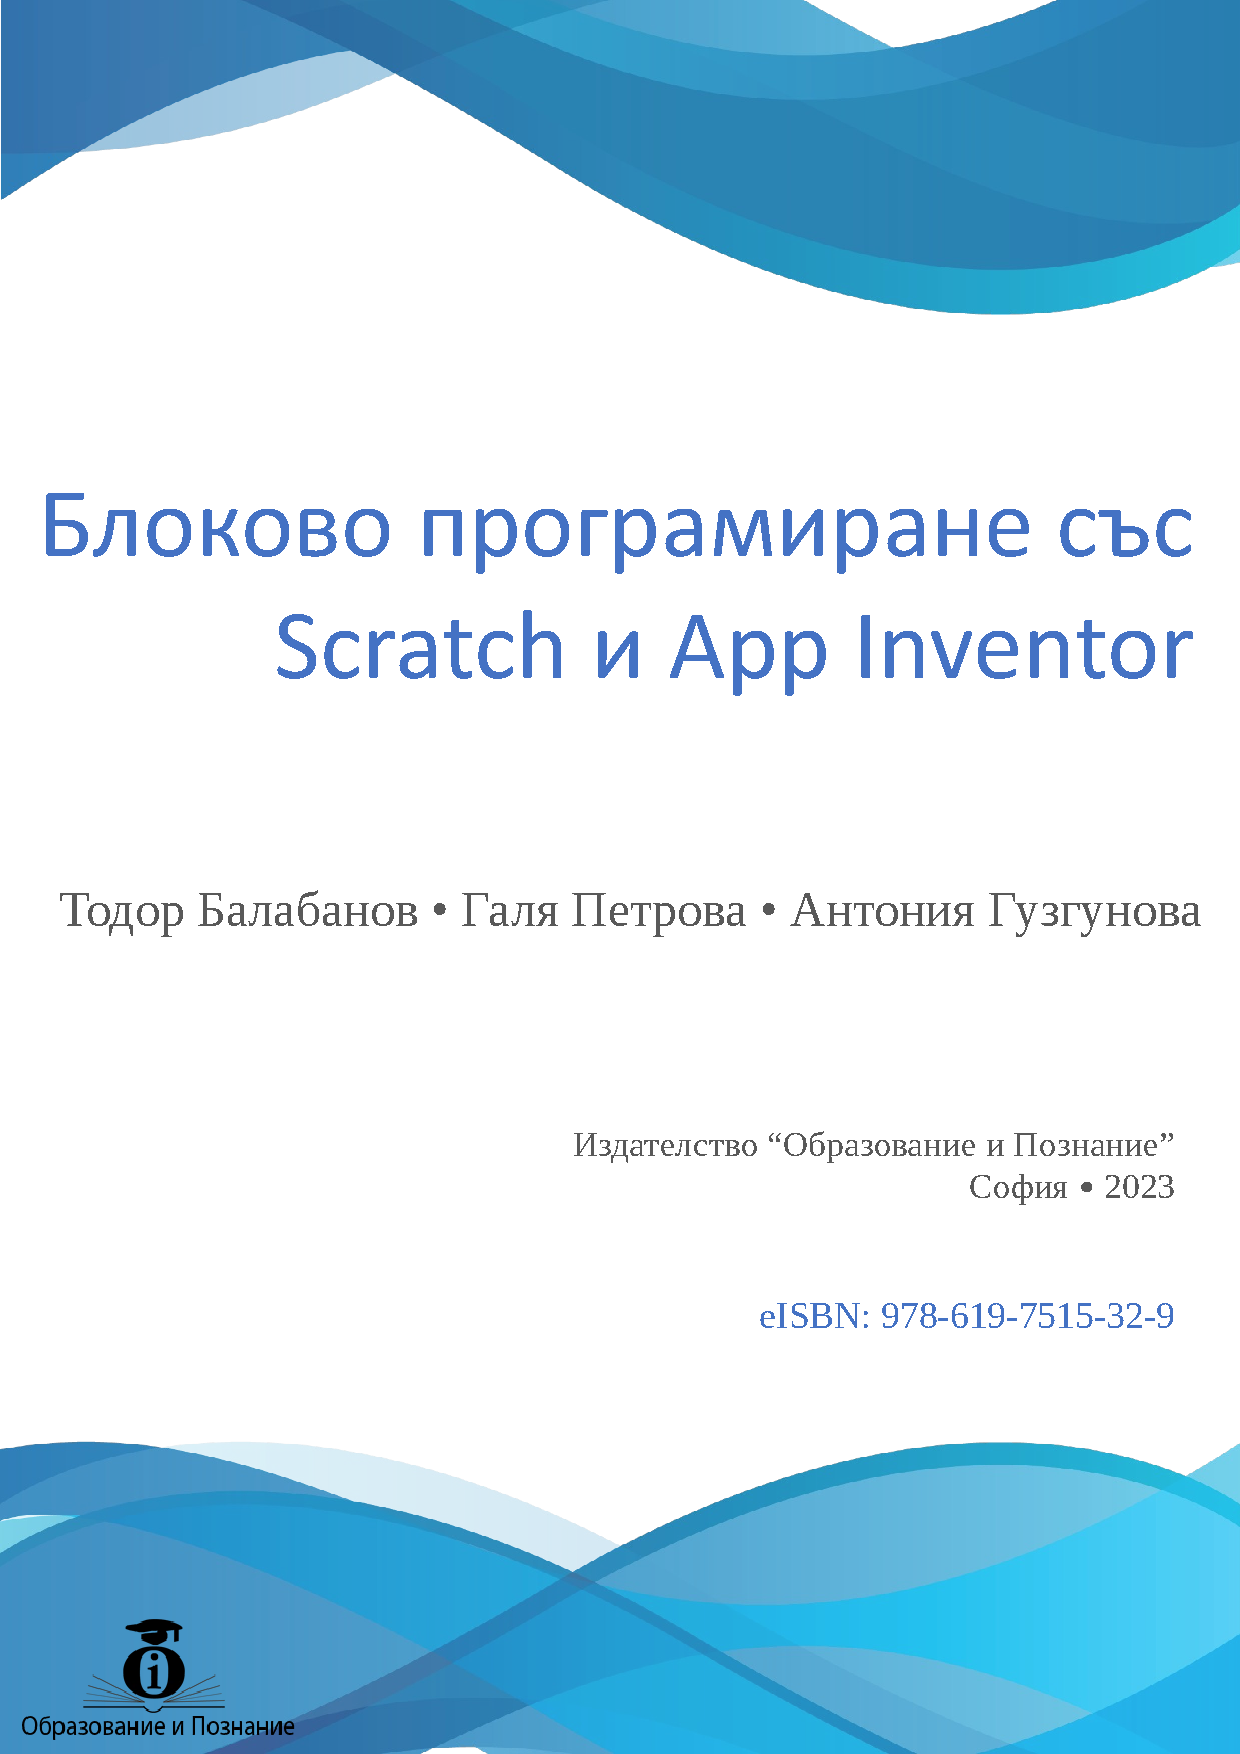
\includepdf[pages={1}]{covers/front}
\thispagestyle{empty}

% Страница с авторски права.
~\vfill
\thispagestyle{empty}

\noindent Авторски права \copyright\ 2022 \\

\noindent Тодор Балабанов, Галя Петрова \\ 

\noindent \textsc{Издателство \say{Образование и Познание}} \\
\noindent \textsc{https://www.obrazovaniebg.net/} \\

\noindent Разпространява се под свободен лиценз: \\ 
Creative Commons Attribution-NonCommercial-NoDerivatives 4.0 \\
International Public License \\
\url{https://creativecommons.org/licenses/by-nc-nd/4.0} \\

\noindent {\footnotesize This book was partially supported by the Bulgarian National Science Fund by the project \say{Mathematical models, methods and algorithms for solving hard optimization problems to achieve high security in communications and better economic sustainability, KP-06-N52/7/19-11-2021}}. \\

\noindent \textit{Първо издание, 2022}

% Номериране на страниците със служебна информация.
\pagenumbering{roman}
\setcounter{page}{1}

% Таблица на съдържанието.
\addcontentsline{toc}{chapter}{Съдържание}
\tableofcontents\newpage

% Списък с фигурите.
\addcontentsline{toc}{chapter}{Списък на фигурите}
\listoffigures\newpage

% Списък с таблиците.
\addcontentsline{toc}{chapter}{Списък на таблиците}
\listoftables\newpage

% Списък с листингите.
\addcontentsline{toc}{chapter}{Списък на листингите}
\lstlistoflistings\newpage

% Номериране на страниците с основното изложение.
\pagenumbering{arabic}
\setcounter{page}{1}

% Отделните глави са в отделни файлове.
\addcontentsline{toc}{chapter}{Предговор}
\chapter*{Предговор}
\thispagestyle{empty}

Тази книга е предназначена за всички хора, които се вълнуват от теми в програмирането и най-вече за обучението на деца в тази област. Надеждата ни е, че всеки с интерес в областта би намерил нещо ценно в изложения материал. Нашият опит е предимно свързан с академичния свят и педагогиката, посветена на обучението на деца. Материалът е изложен по такъв начин, че да разкрива основните механизми за учене чрез правене. Най-общо казано, книгата съпровожда читателя с минимални компютърни познания до едно задоволително ниво на разбиране за концепциите в програмирането. 

От наша гледна точка, представянето на програмните конструкции с помощта на визуализация, максимално доближаваща класическите пъзели, дава широки възможности за усвояване на ценни знания и умения. Подобен подход за онагледяване позволява ефективно снижаване на възрастта за обучение по програмиране. Докато класическите програмни езици са подходящи в класовете на гимназията, блоковите езици ефективно намират своето приложение в прогимназиалния курс на обучение. 

Част от изложения материал разяснява фундаментални концепции в програмирането, като - последователност от инструкции, условни и безусловни преходи, цикличност на действията, събития, модулна организация и други. Друга част набляга на практическа реализация и то на идеи, които имат потенциал да се превърнат в самостоятелни софтуерни решения. Избраният подход за представяне на информацията е чрез примери на принципа – направа, стъпка по стъпка. 

Книгата не предполага предварителни изисквания за напреднало ниво на компютърна грамотност, но разчита читателят да има базови познания за това какво е компютърна система, какво е операционна система, какво е Интернет, как се борави със зареждането и преглеждането на уеб страници. Разгледаните системи за блоково програмиране са уеб базирани и работата с тях се осъществява в облачно пространство. Не се изискват задълбочени познания по математика, но за разбирането на някои от примерите много помагат базови познания по алгебра и геометрия. Артистични умения, като музикалност или изобразителни изкуства не са нужни, но наличието им би дало допълнителен колорит на постигнатите резултати. 

Материалът е организиран в глави, които са свързани една с друга и за по-пълноценно усвояване е желателно прочитането им да се извърши в зададената последователност. Част от изложението в книгата се базира на учебни предмети, преподавани в прогимназиалния курс на обучение.

\vspace{0.5cm}

\large{\textbf{Благодарности}}

\vspace{0.5cm}

Авторите биха искали да благодарят на своите семейства за търпението и разбирането, проявено в дългият период за написването на тази книга. Също така биха искали да благодарят на своите колеги и приятели, помогнали в достигането на едно по-високо качество. 



\newpage
%\chapter{Работни среди}

Блоковите програмни езици са подразделение на визуалните програмни езици. Същината на блоковите езици е, че програмните инструкции се въвеждат под формата на цветни блокове, а не както е в класическите програмни езици, чрез изписване на текстови команди. Най-основната цел на блоковите езици е да направят областта програмиране значително по-достъпна за начинаещите. Тази цел се постига чрез три основни направления. От синтактична гледна точка, инструкциите в блоковите езици са под формата на цветни иконки. Това значително намалява възможността за изписването на грешна програмна инструкция. На второ място се подобрява семантиката, като всяка от възможните програмни инструкции е добре документирана. На трето място е прагматизма, който позволява изучаването на различните състояния в които може да изпадне програмата. Програмните среди за блоково програмиране набират все по-голяма популярност през последното десетилетие. Някои от най-популярните са: Scratch, Blockly, App Inventor for Android, Ardublock и други. В тази книга ще се спрем на две от програмните среди за блоково програмиране, създадени в Масачузетския технологичен институт, Scratch и App Inventor for Android. Причината за този избор е, че Scratch има насоченост към най-малките, а именно децата в началните училищни класове, което много добре се съчетава с възможностите блоковите програми да бъдат визуализирани и на мобилен телефон, чрез App Inventor for Android. И при двете програмни среди не се изисква инсталирането на специализиран софтуер. Достатъчно е наличието на съвременен компютър, свързан в Интернет и съвременна версия на уеб браузър. 

\section{Първи стъпки в Sratch}

Работата в средата на Sratch започва със зареждане на главната уеб страница (Фиг. \ref{fig0001}), която се намира на адрес: \\ \href{https://scratch.mit.edu/}{https://scratch.mit.edu/}

\begin{figure}[H]
  \centering
  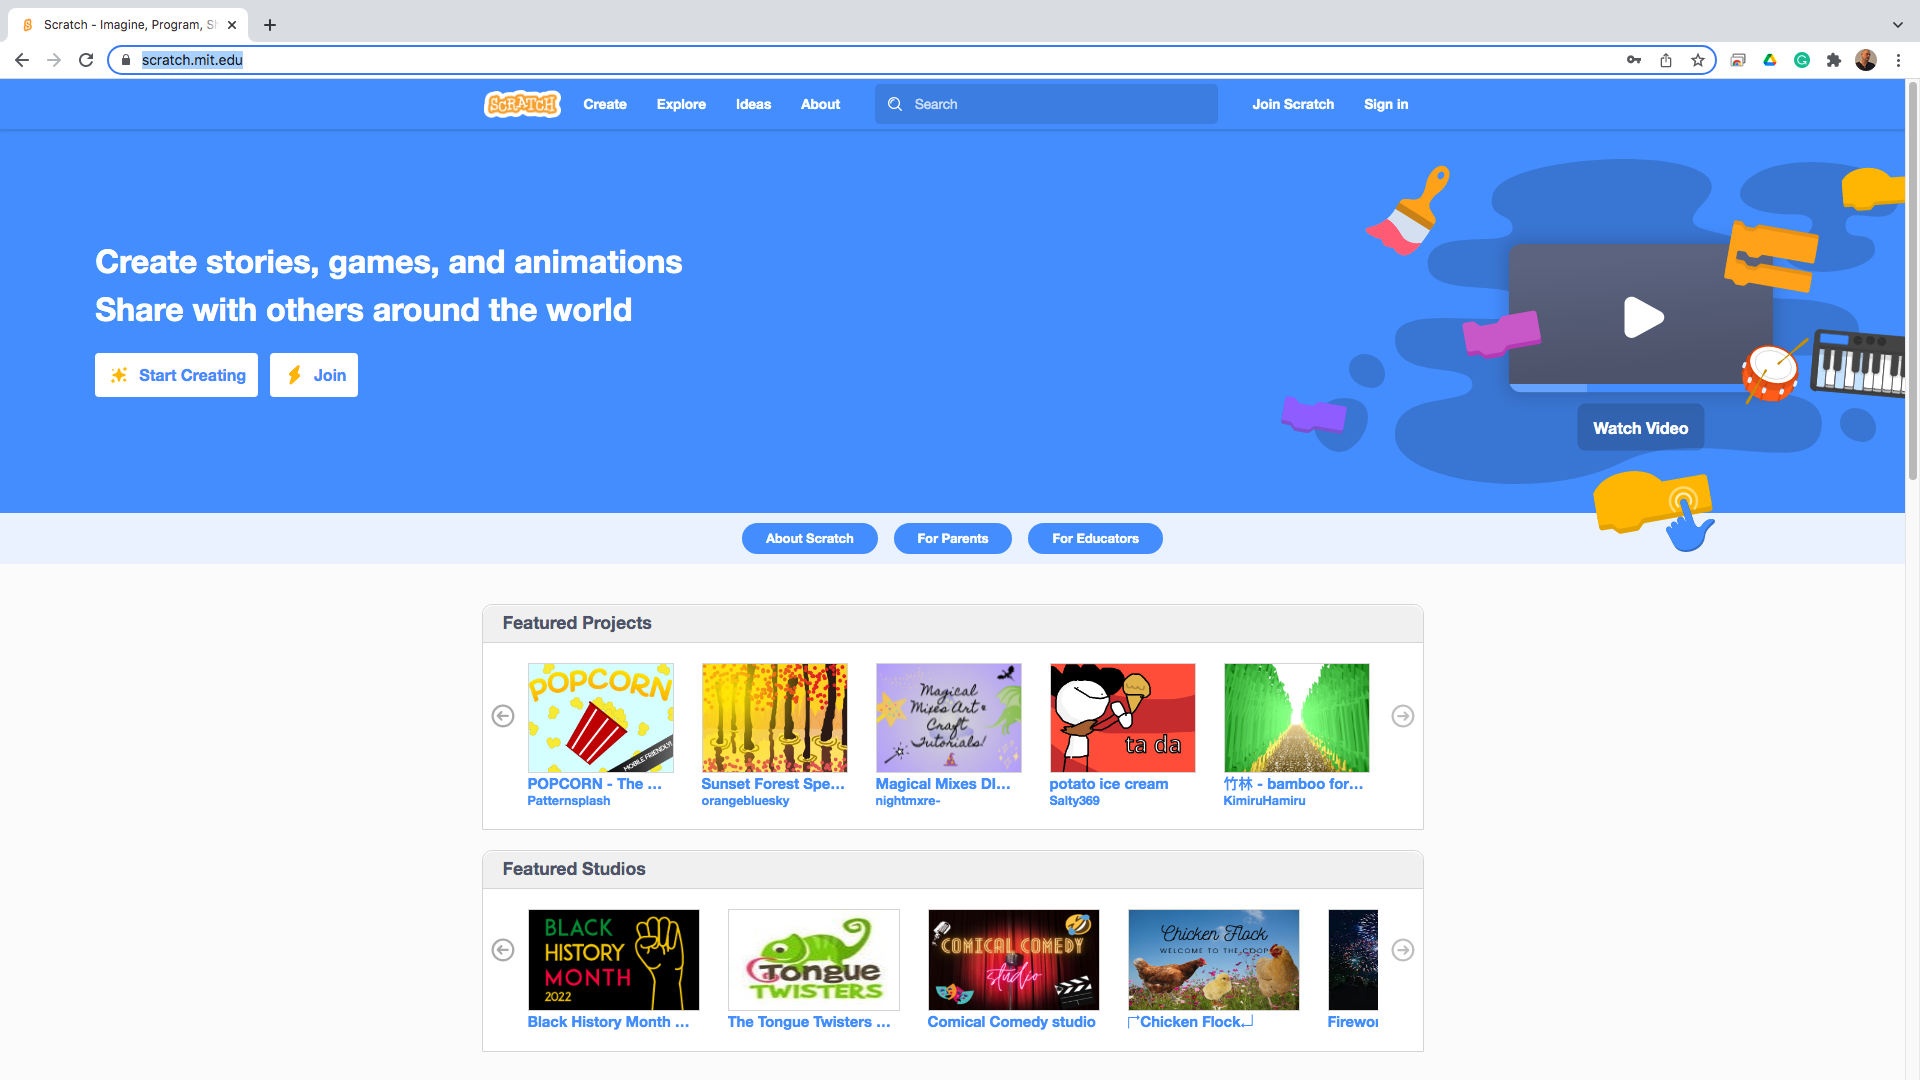
\includegraphics[width=1.0\linewidth,height=0.5\linewidth]{fig0001.png}
  \caption{Начална уеб страница на Sratch}
\label{fig0001}
\end{figure}

Програмната среда на Sratch е организирана на принципа на облачните услуги. Поради тази причина, всеки желаещ да използва услугата трябва да си направи регистрация (Фиг. \ref{fig0002}). Регистрацията се състои от потребителско име и парола.

\begin{figure}[H]
  \centering
  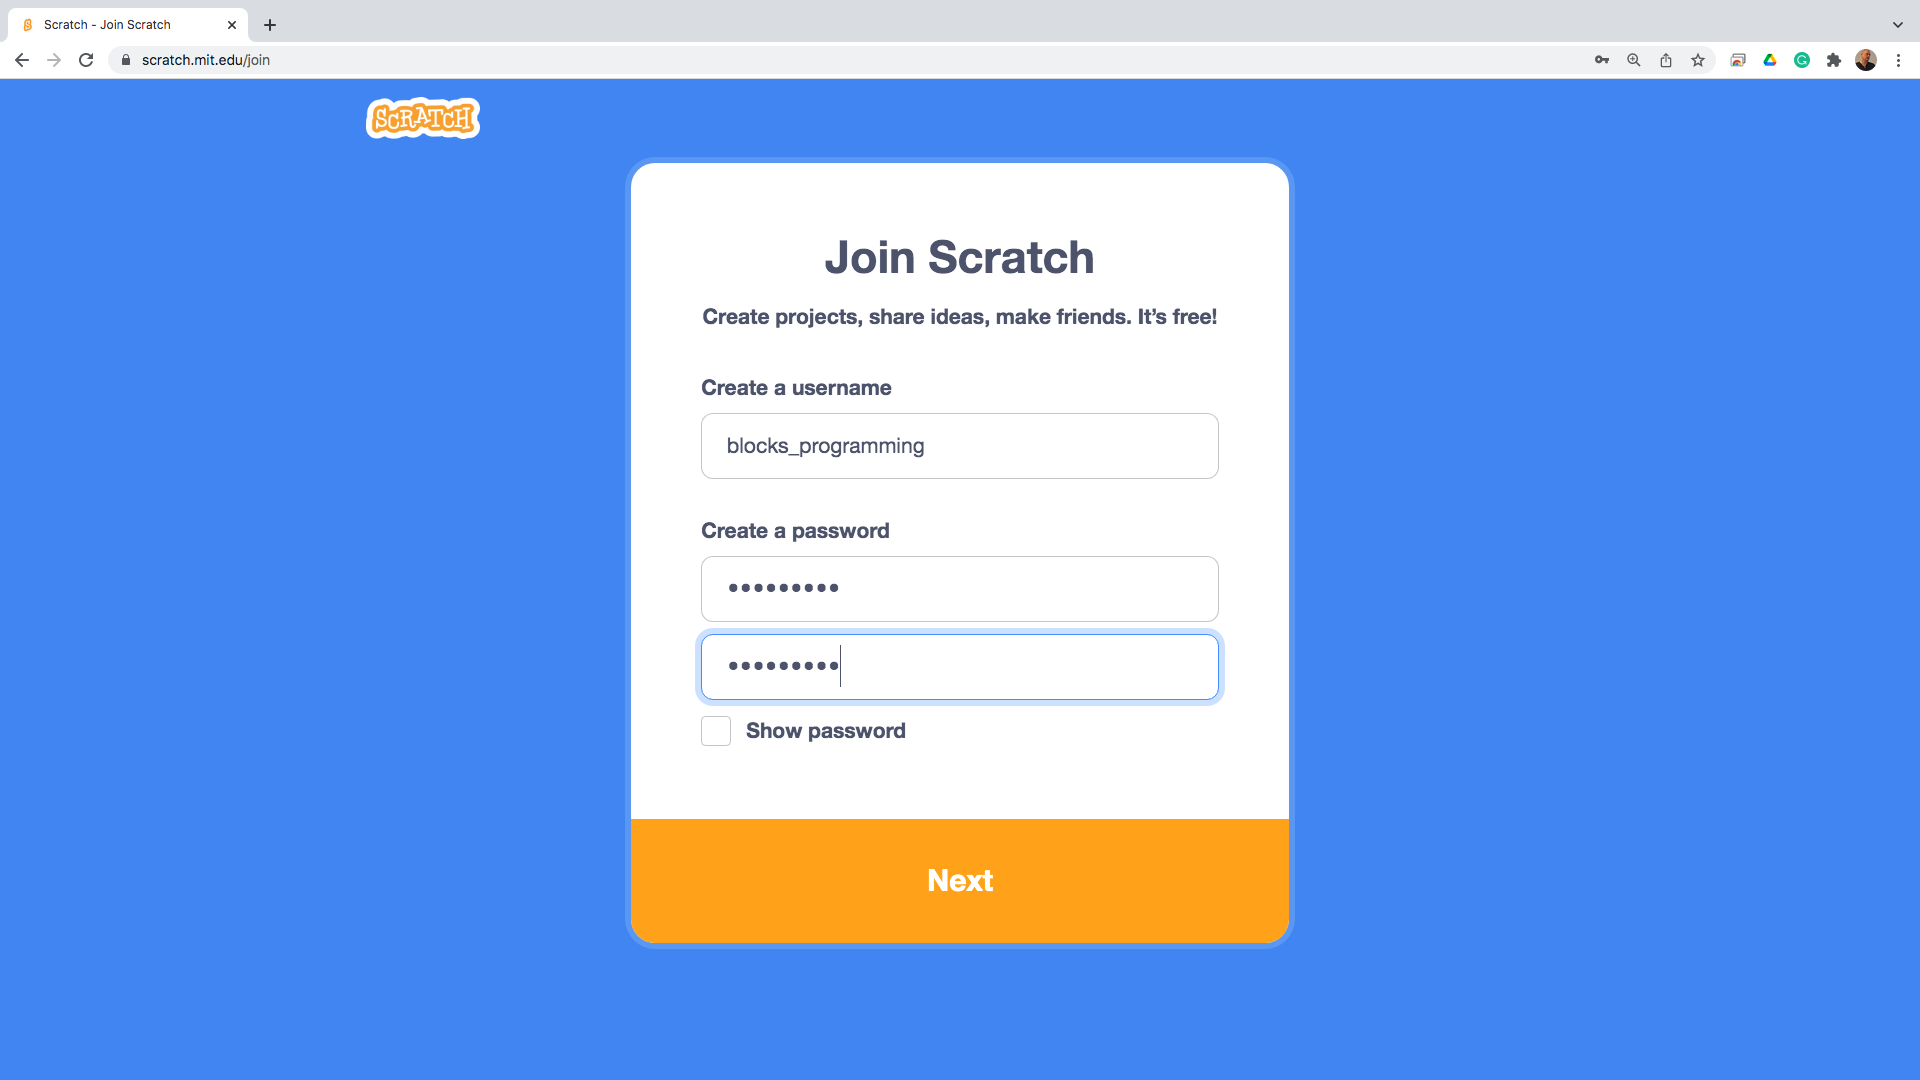
\includegraphics[width=1.0\linewidth,height=0.5\linewidth]{fig0002.png}
  \caption{Регистрация на потребител в Sratch}
\label{fig0002}
\end{figure}

След избора на потребителско име и парола следва определяне на географския регион в който се намира потребителят (Фиг. \ref{fig0003}).

\begin{figure}[H]
  \centering
  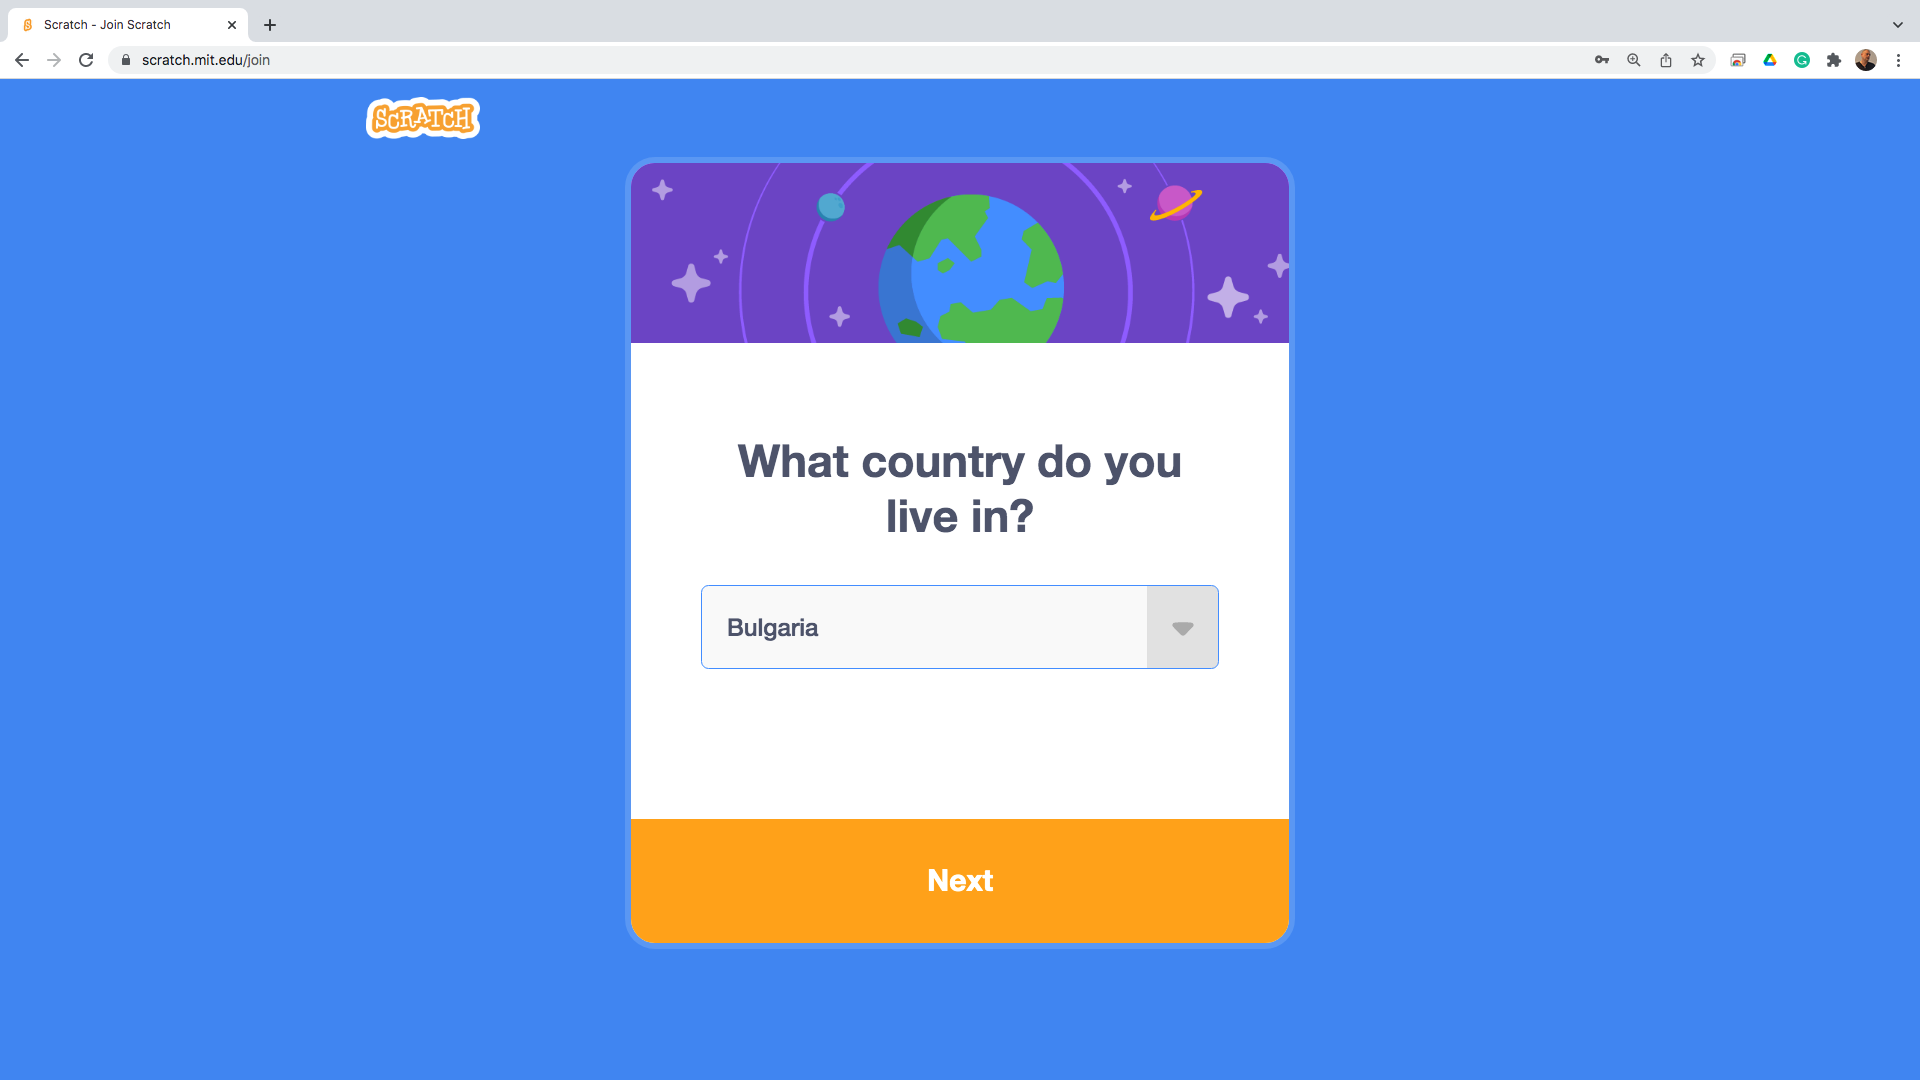
\includegraphics[width=1.0\linewidth,height=0.5\linewidth]{fig0003.png}
  \caption{Географско местоположение}
\label{fig0003}
\end{figure}

Платформата е насочена предимно към деца, изразяващи интерес към програмирането, но също така към родители и учители. Поради тази причина, системата събира информация за възрастта на потребителя (Фиг. \ref{fig0004}).

\begin{figure}[H]
  \centering
  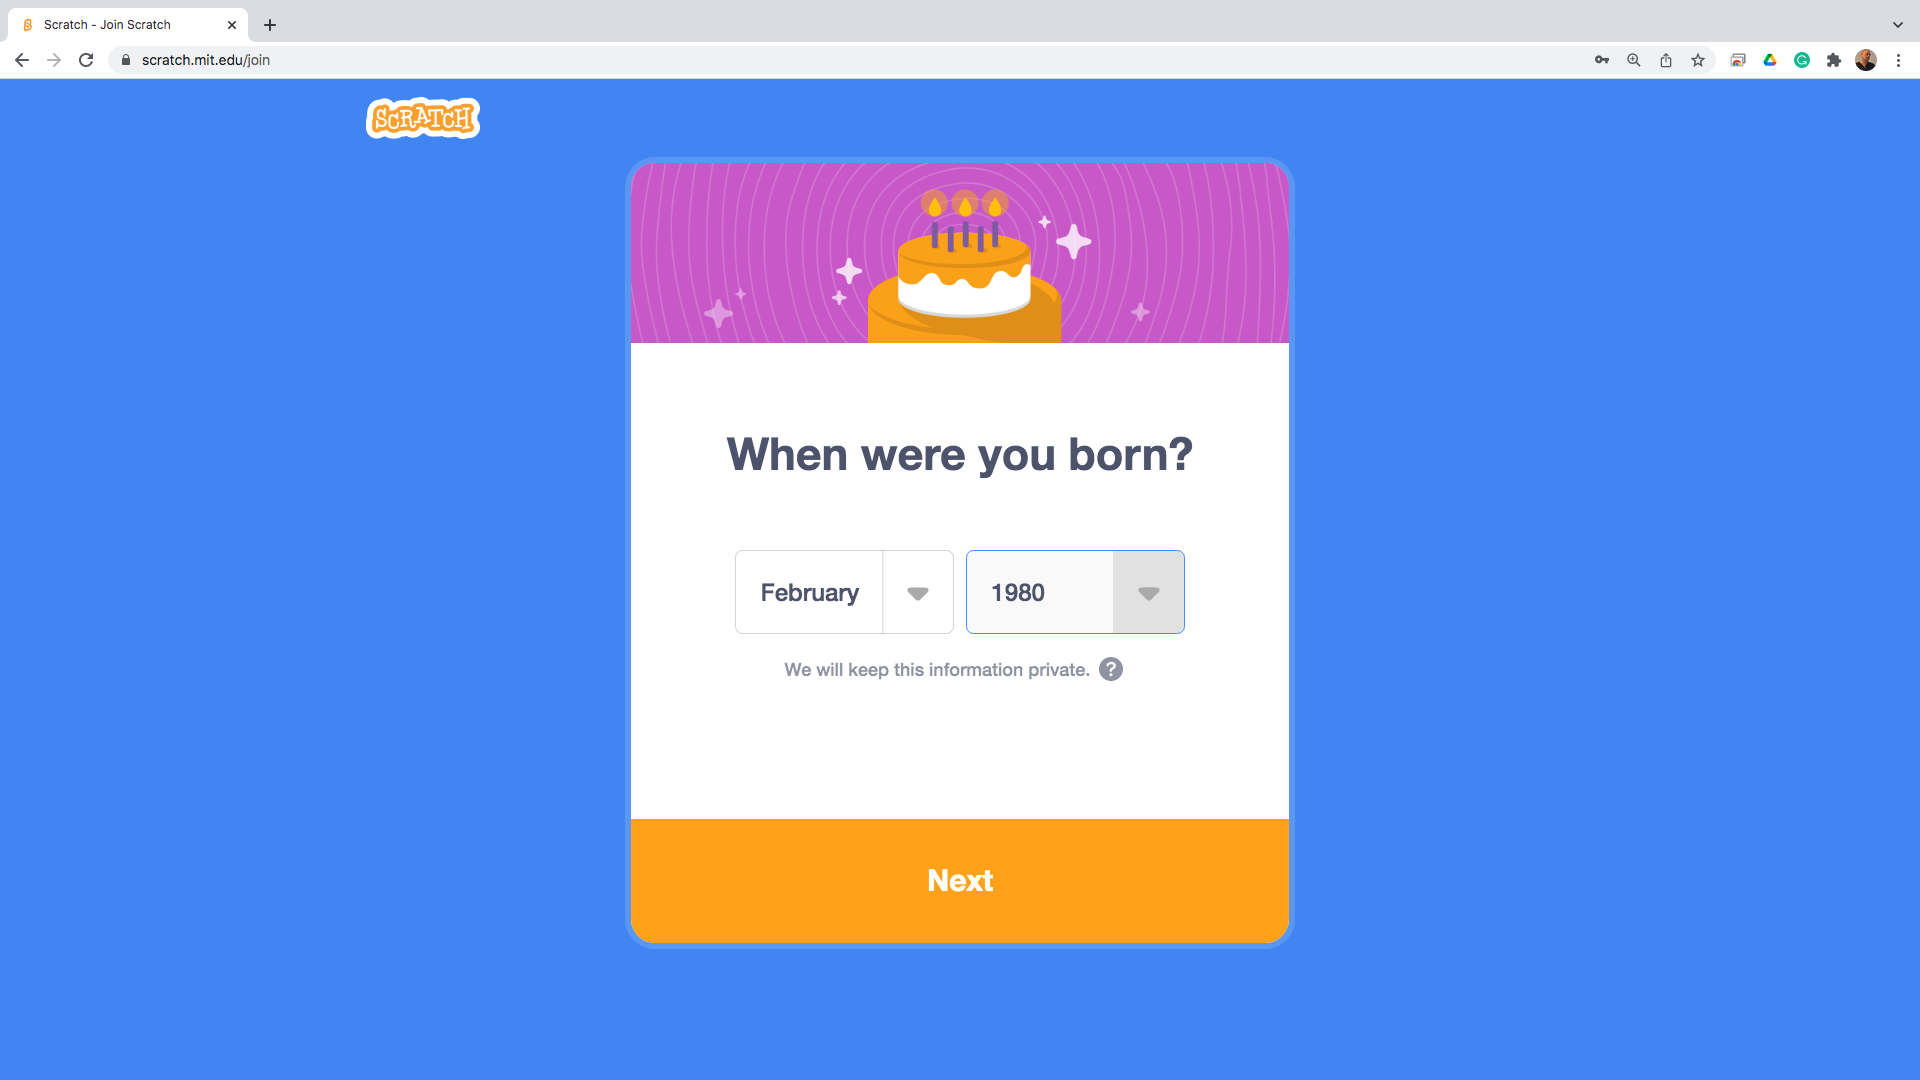
\includegraphics[width=1.0\linewidth,height=0.5\linewidth]{fig0004.png}
  \caption{Възраст на потребителя}
\label{fig0004}
\end{figure}

Освен класификация по възраст, системата събира информация и за класификация по полова принадлежност. Тази информация е незадължителна, основно за да не бъде дискриминираща (Фиг. \ref{fig0005}).

\begin{figure}[H]
  \centering
  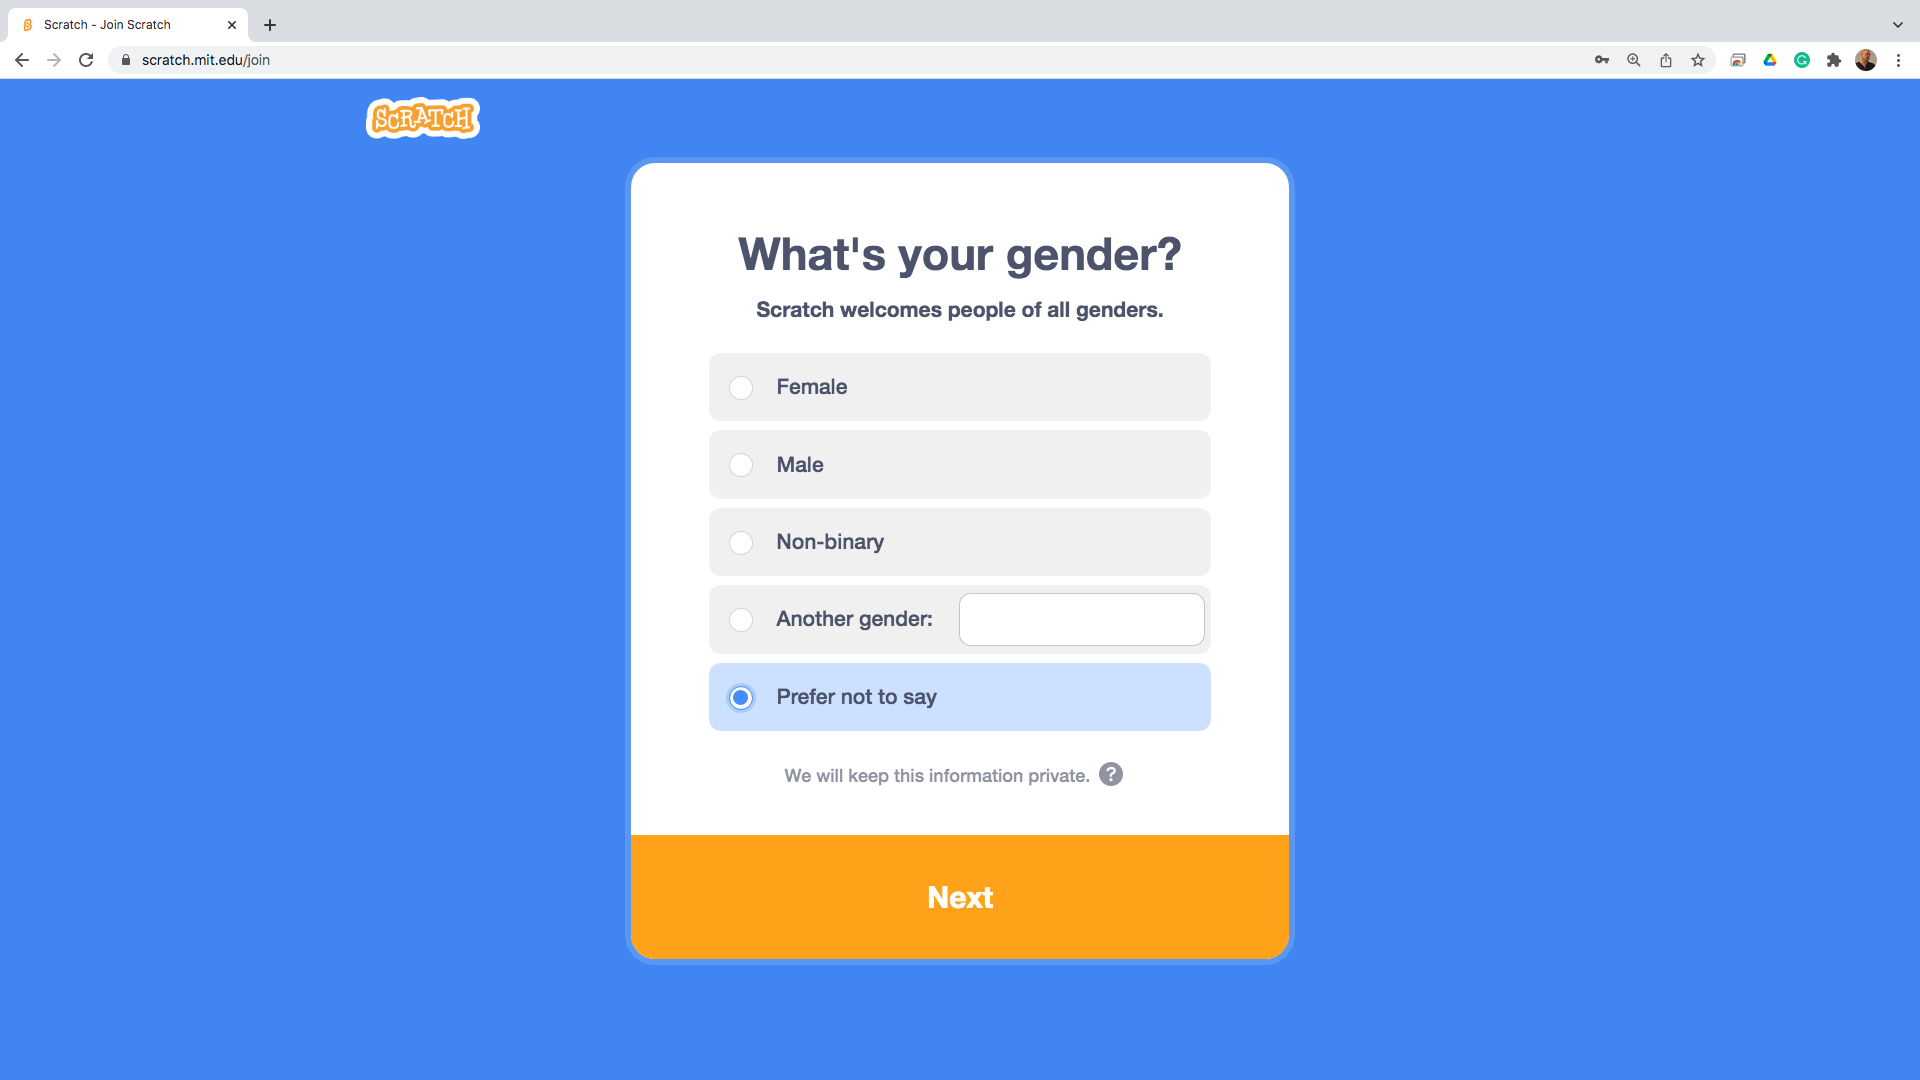
\includegraphics[width=1.0\linewidth,height=0.5\linewidth]{fig0005.png}
  \caption{Пол на потребителя}
\label{fig0005}
\end{figure}

Потребителският профил, освен с потребителско име и парола, трябва да бъде аоцииран и с адрес на електронна пощенска кутия (Фиг. \ref{fig0006}).

\begin{figure}[H]
  \centering
  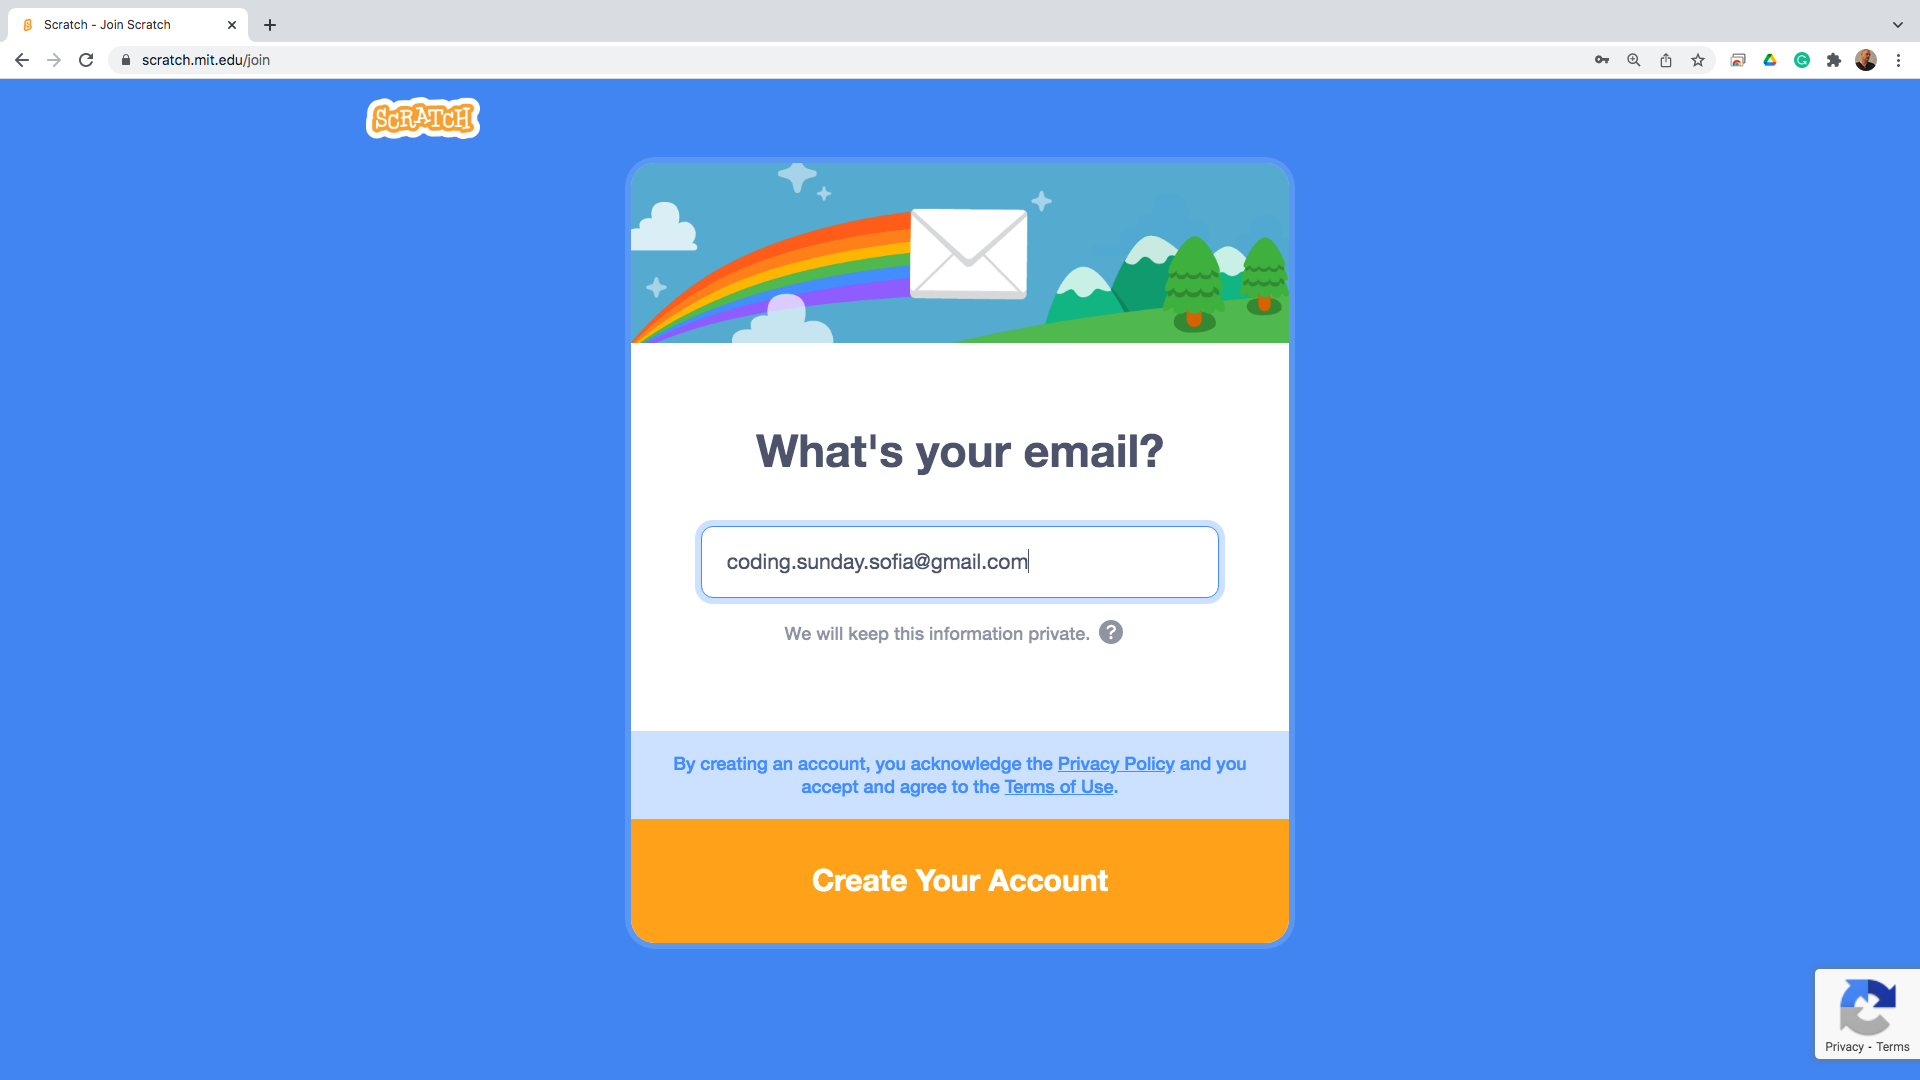
\includegraphics[width=1.0\linewidth,height=0.5\linewidth]{fig0006.png}
  \caption{Адрес на електронна поща на потребителя}
\label{fig0006}
\end{figure}

Процесът по регистрация на потребител в системата е почти завършен (Фиг. \ref{fig0007}). Остава само стъпката за потвърждаване на избрания адрес за електронна поща.

\begin{figure}[H]
  \centering
  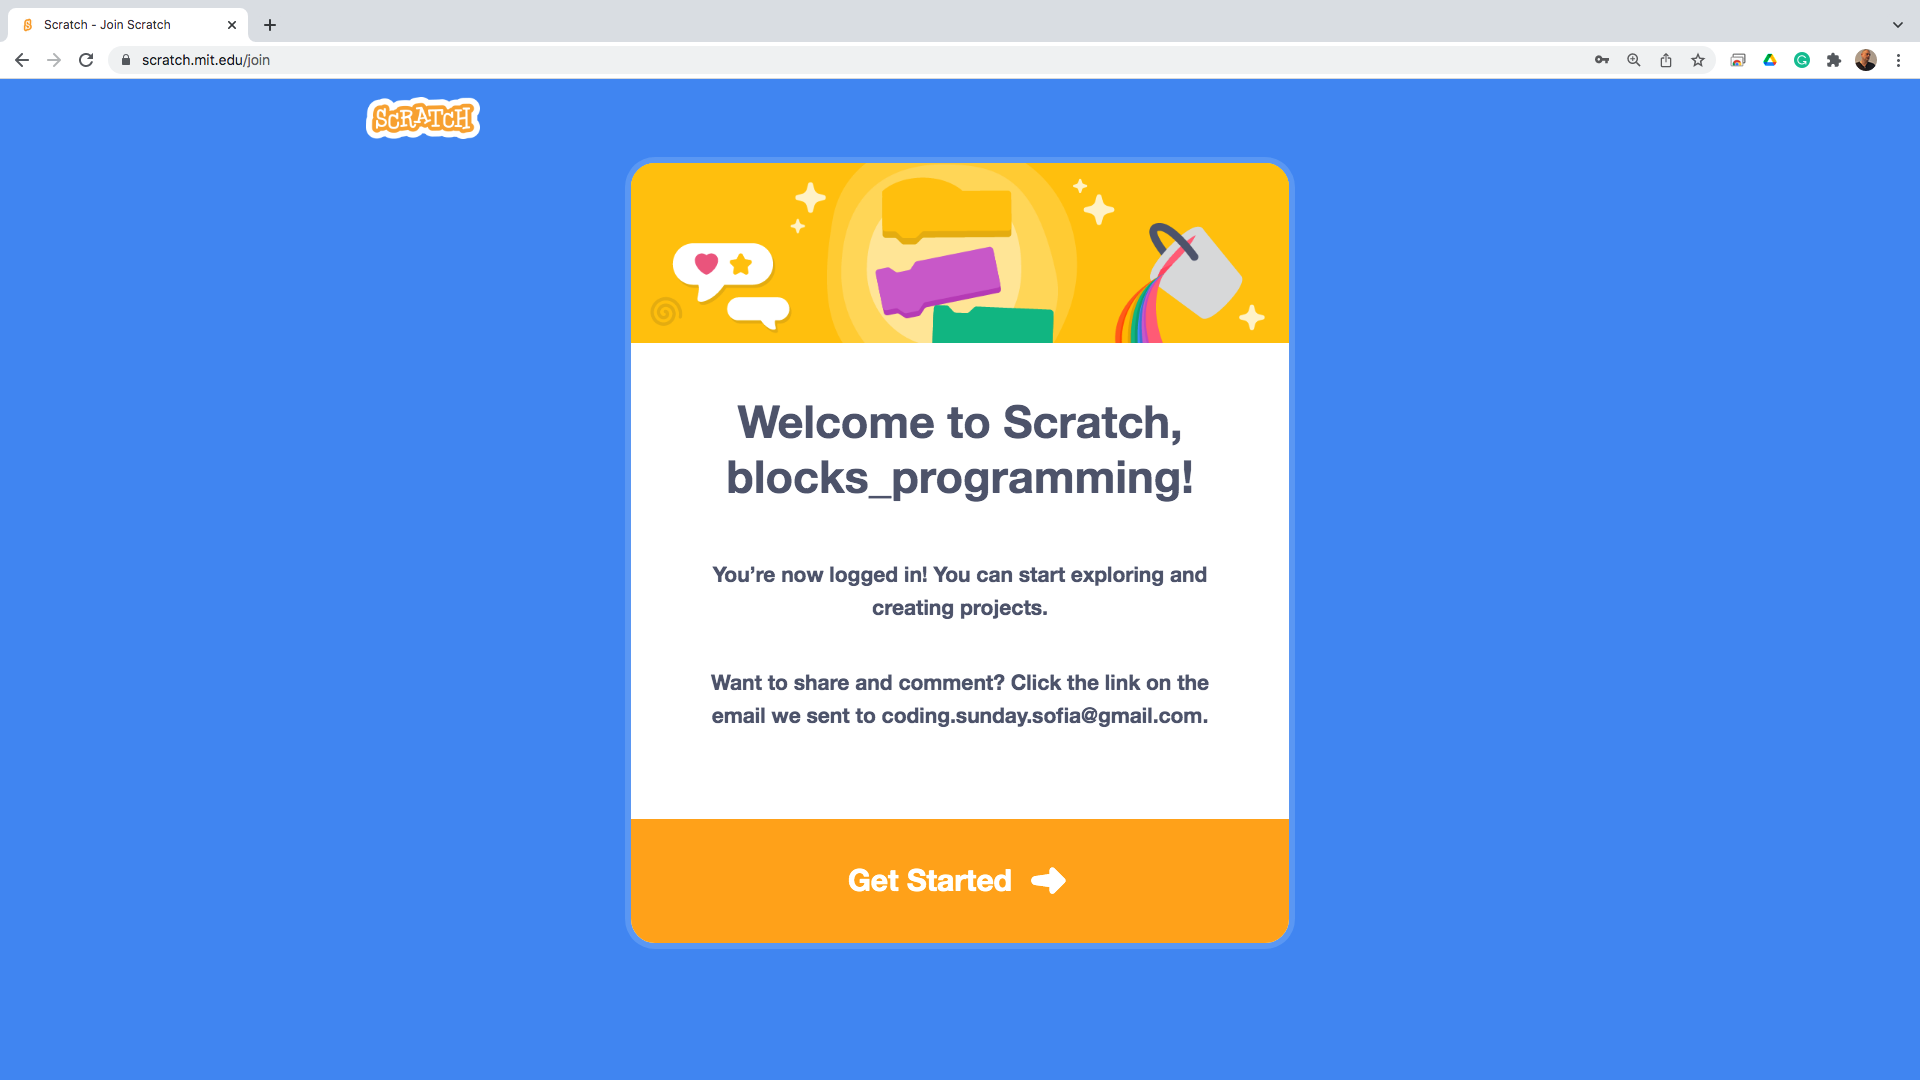
\includegraphics[width=1.0\linewidth,height=0.5\linewidth]{fig0007.png}
  \caption{Приключване на процеса за въвеждане на информация за потребителя}
\label{fig0007}
\end{figure}

Електронното писмо, за потвърждаване на потребителската регистрация, съдържа електронна препратка до уеб сайта на Sratch (Фиг. \ref{fig0008}). Тази препратка трябва да бъде последвана за да се завърши процесът по регистрация на нов потребител. 

\begin{figure}[H]
  \centering
  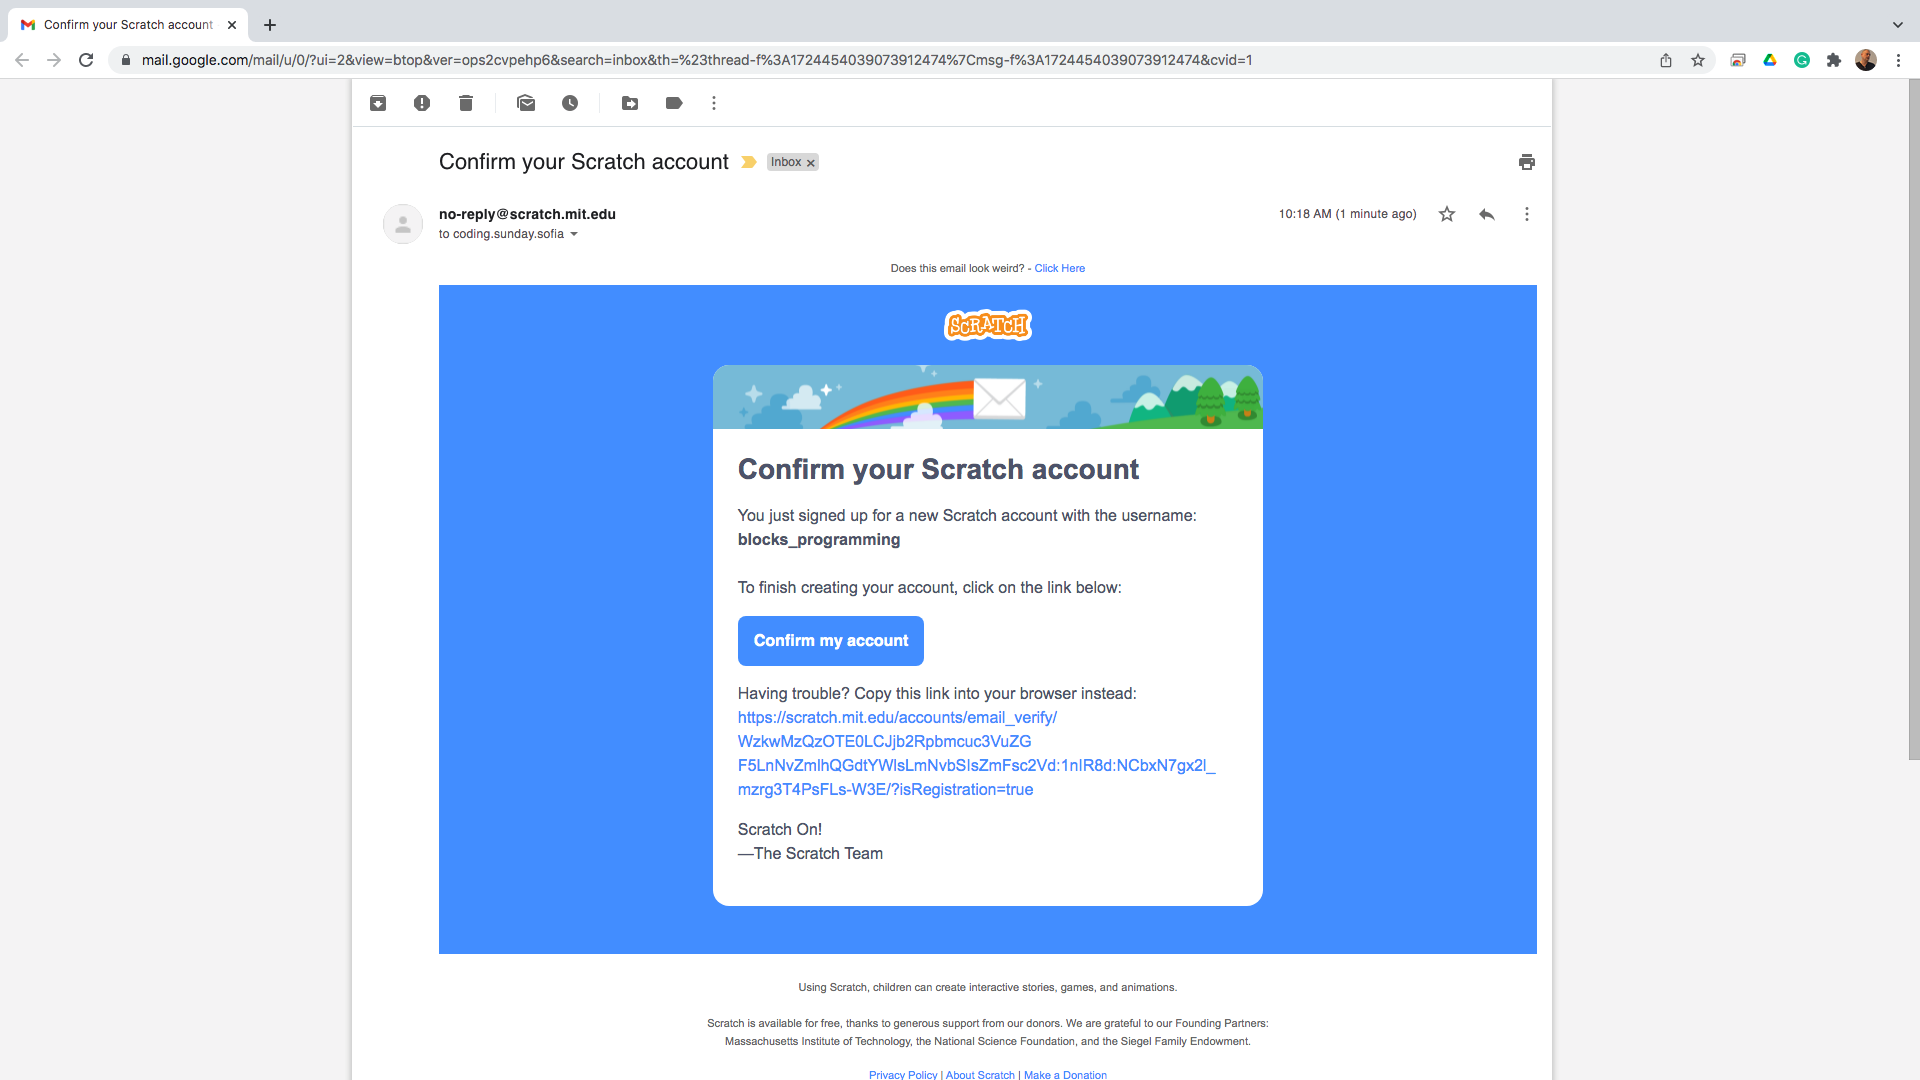
\includegraphics[width=1.0\linewidth,height=0.5\linewidth]{fig0008.png}
  \caption{Електронно съобщение за потвърждаване на електронния адрес}
\label{fig0008}
\end{figure}

Регистрацията на новия потребител приключва със зареждането на начален работен екран (Фиг. \ref{fig0009}). Горе, в дясно се вижда изписано потребителското име, избрано на първата стъпка от процеса по регистрацията.

\begin{figure}[H]
  \centering
  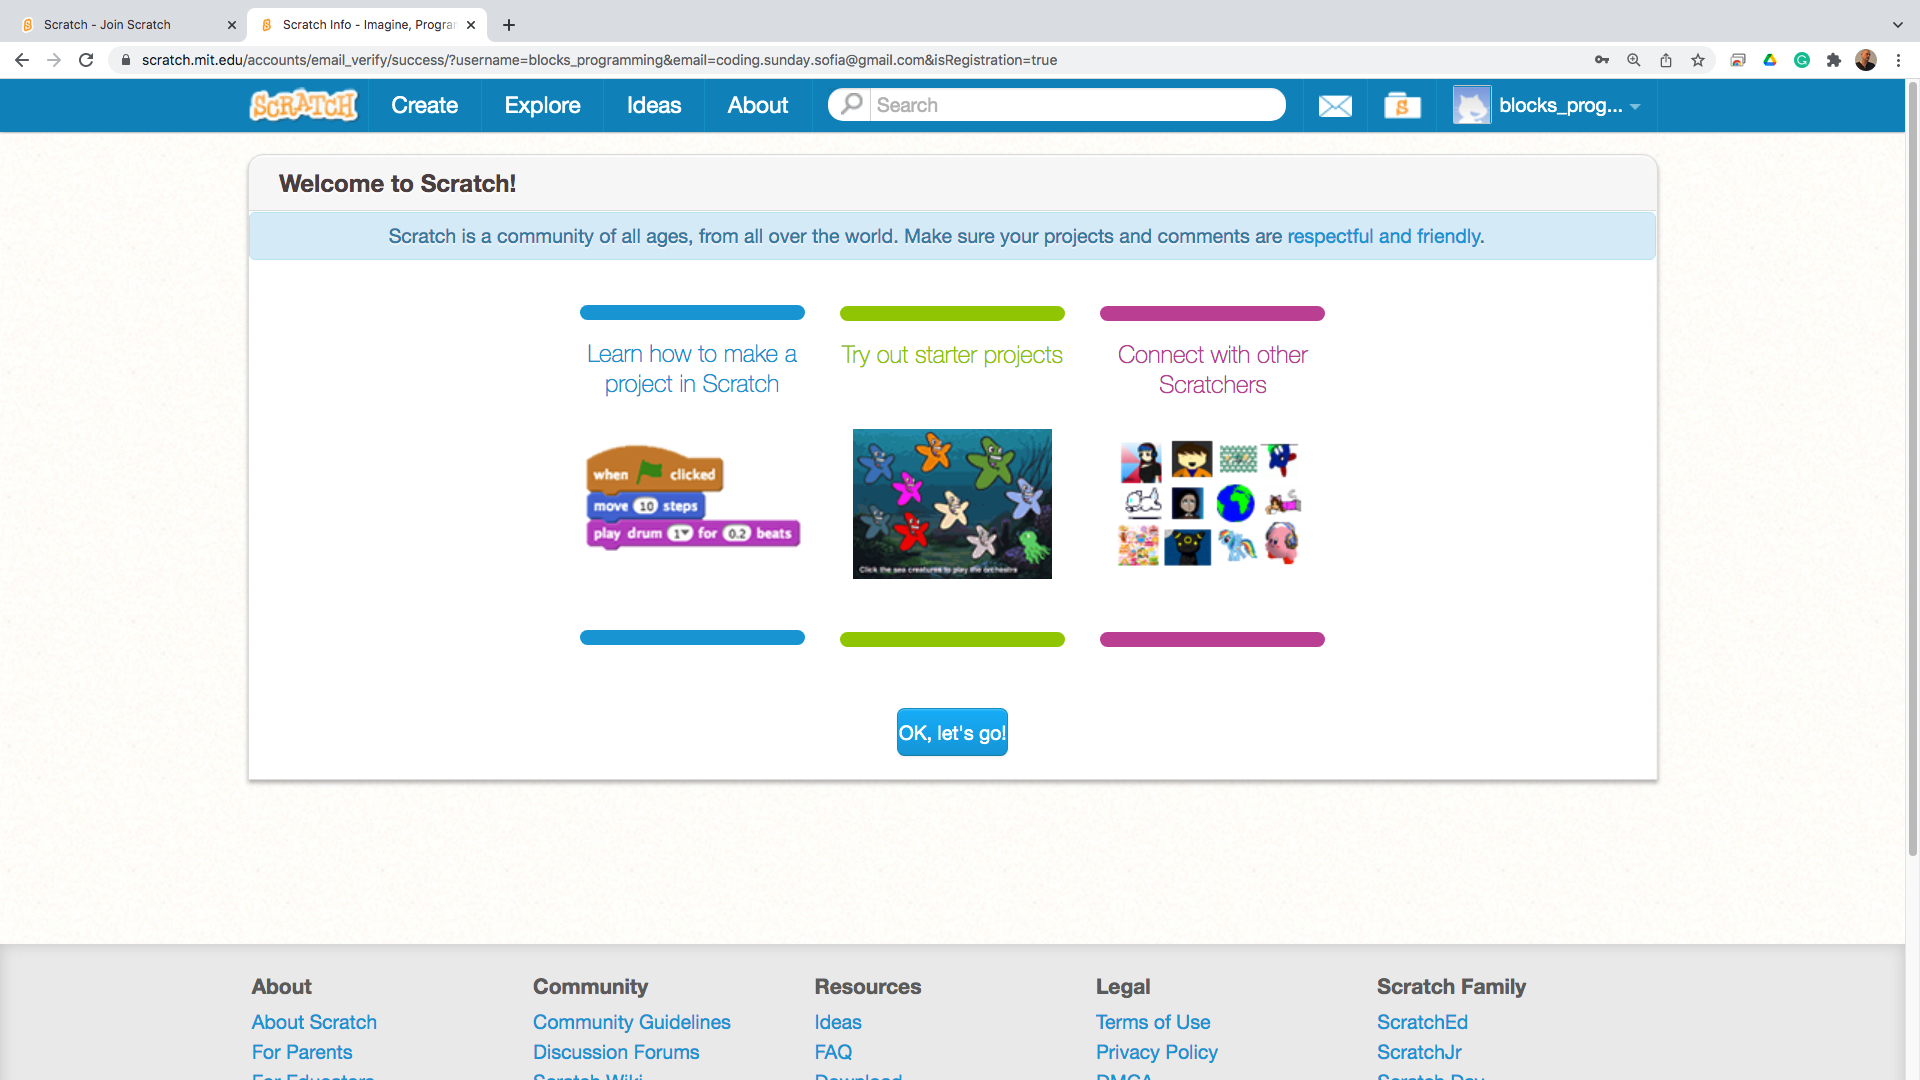
\includegraphics[width=1.0\linewidth,height=0.5\linewidth]{fig0009.png}
  \caption{Начален работен екран}
\label{fig0009}
\end{figure}

\section{Първи стъпки в App Inventor}

\newpage
\chapter{Програмни конструкции}

Компютърните програми са съставени от стриктна последователност инструкции. Такива последователности се наричат алгоритъм. Ние хората всеки ден изпълняваме различни алгоритми, като част от нашето ежедневие. Да се приготвим и да отидем на училище е един алгоритъм. Събуждаме се, ставаме, обличаме се, правим си сутрешния тоалет, закусваме, излизаме от вкъщи, придвижваме се до училище. Много ярък пример за алгоритъм са рецептите за готвене. В една рецепта има начални продукти, след това точни инструкции как продуктите са се обработят и смесят, като има ясна представа какъв трябва да бъде крайният резултат. При компютърните програми има основен набор от инструкции, които съставляват изразните средства на съответния програмен език. Чарът на блоковите езици е, че този основен набор от инструкции е представен визуално, под формата на цветни блокчета. Подредбата на цветните блокчета в строго определена последователност води до създаването на малки компютърни програми. 

В случая на Scratch, програмата има ясно определена стартова точка и ясно определена финална точка. При App Inventor подходът е малко по-различен. Там последователността от инструкции, съставляващи писаната програма, се въвежда в малки фрагменти, наречени събития. Събитията възникват при различни действия от страна на потребителя или операционната система. При Scratch говорим за последователно програмиране, а при App Inventor говорим за събитийно програмиране. Основните програмни конструкции в двете програмни среди до голяма степен са идентични, но има и някои съществени разлики. За да можем да пишем ефективни и надеждни програми е важно добре да познаваме изразните средства на програмните среди с които работим. 

\section{Изразни средства в Scratch}

Базовите градивни блокчета в Scratch са организирани в цветни групи (Фиг. \ref{fig0051}). Тази организация помага за по-бързо ориентиране и по-ефективна употреба на различните блокчета. 

\begin{figure}[H]
  \centering
  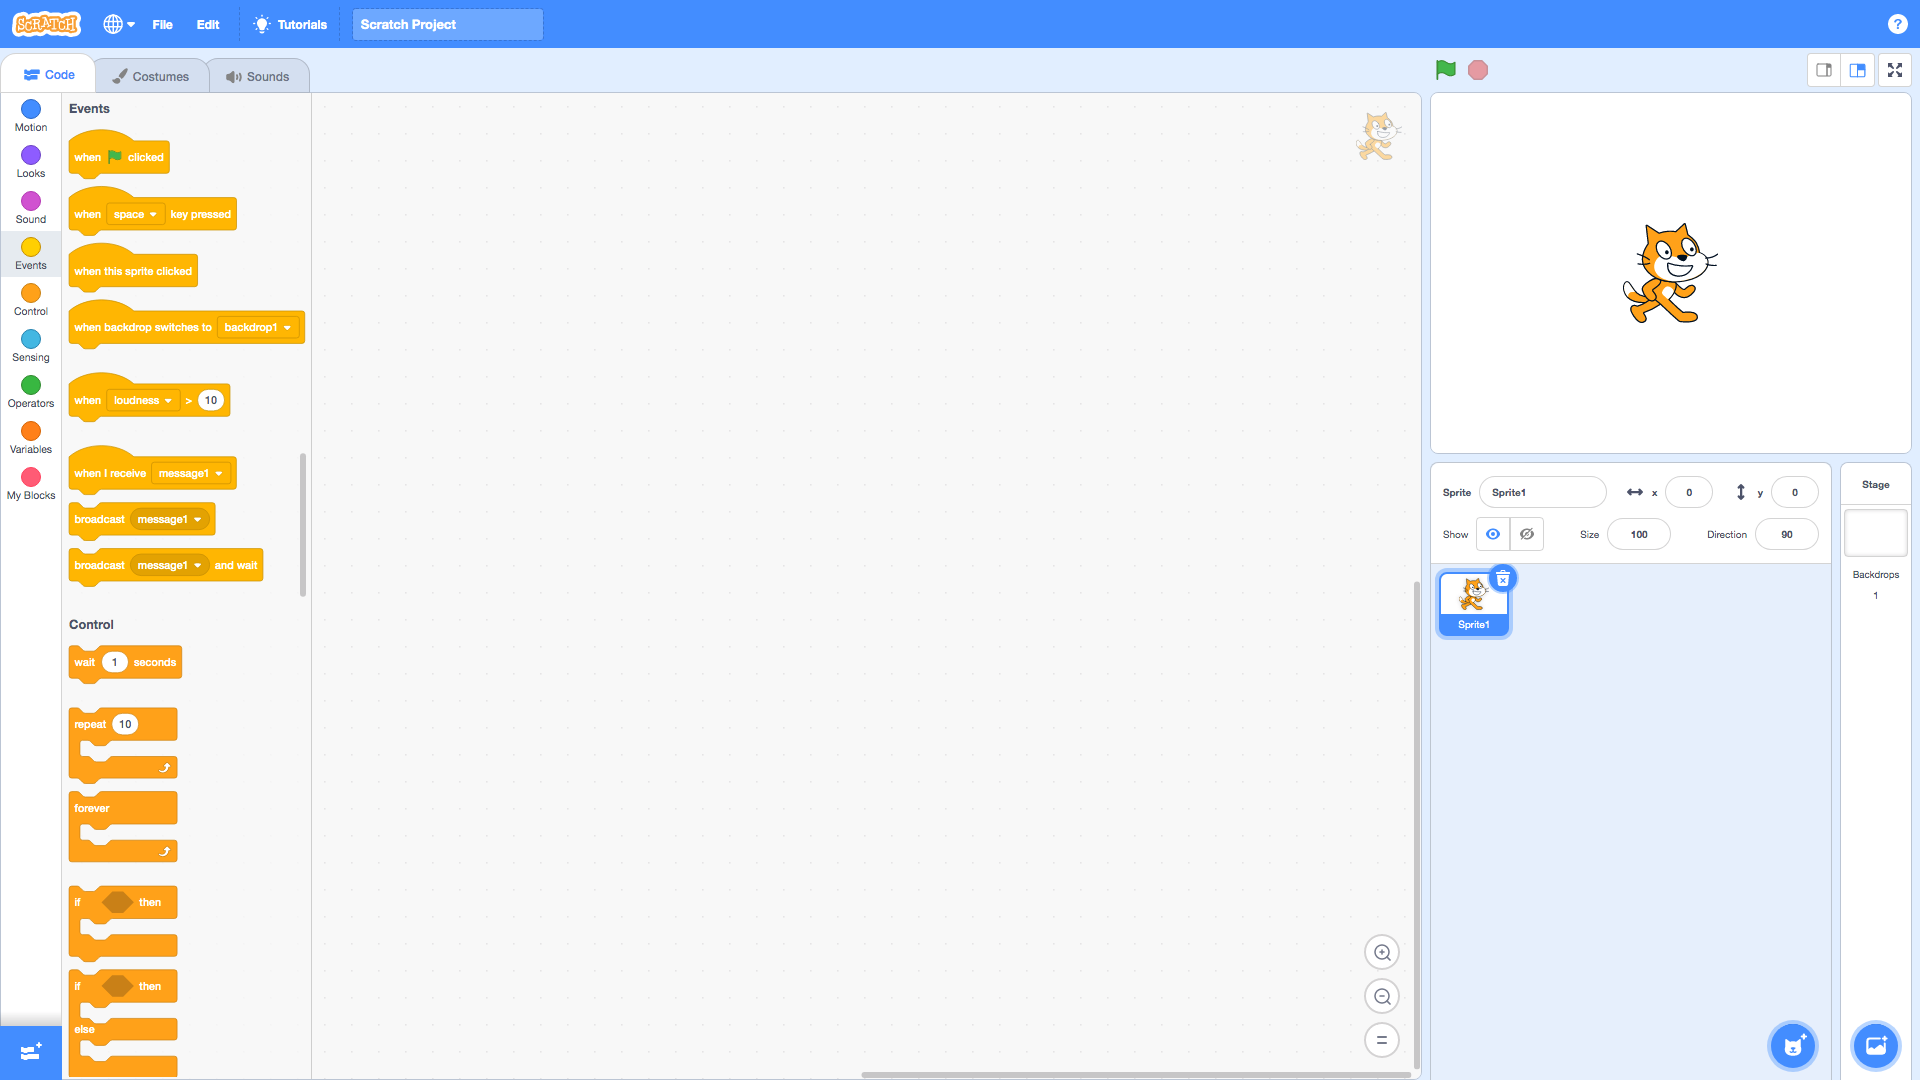
\includegraphics[width=1.0\linewidth,height=0.5\linewidth]{fig0051.png}
  \caption{Групиране на инструкциите}
\label{fig0051}
\end{figure}

Най-важното блокче в програмата е блокчето, което дава старт за изпълнение на инструкциите, които са подредени под него. Това блокче има зелен флаг (Фиг. \ref{fig0052}) и определя какво ще последва след стартирането на програмата.

\begin{figure}[H]
  \centering
  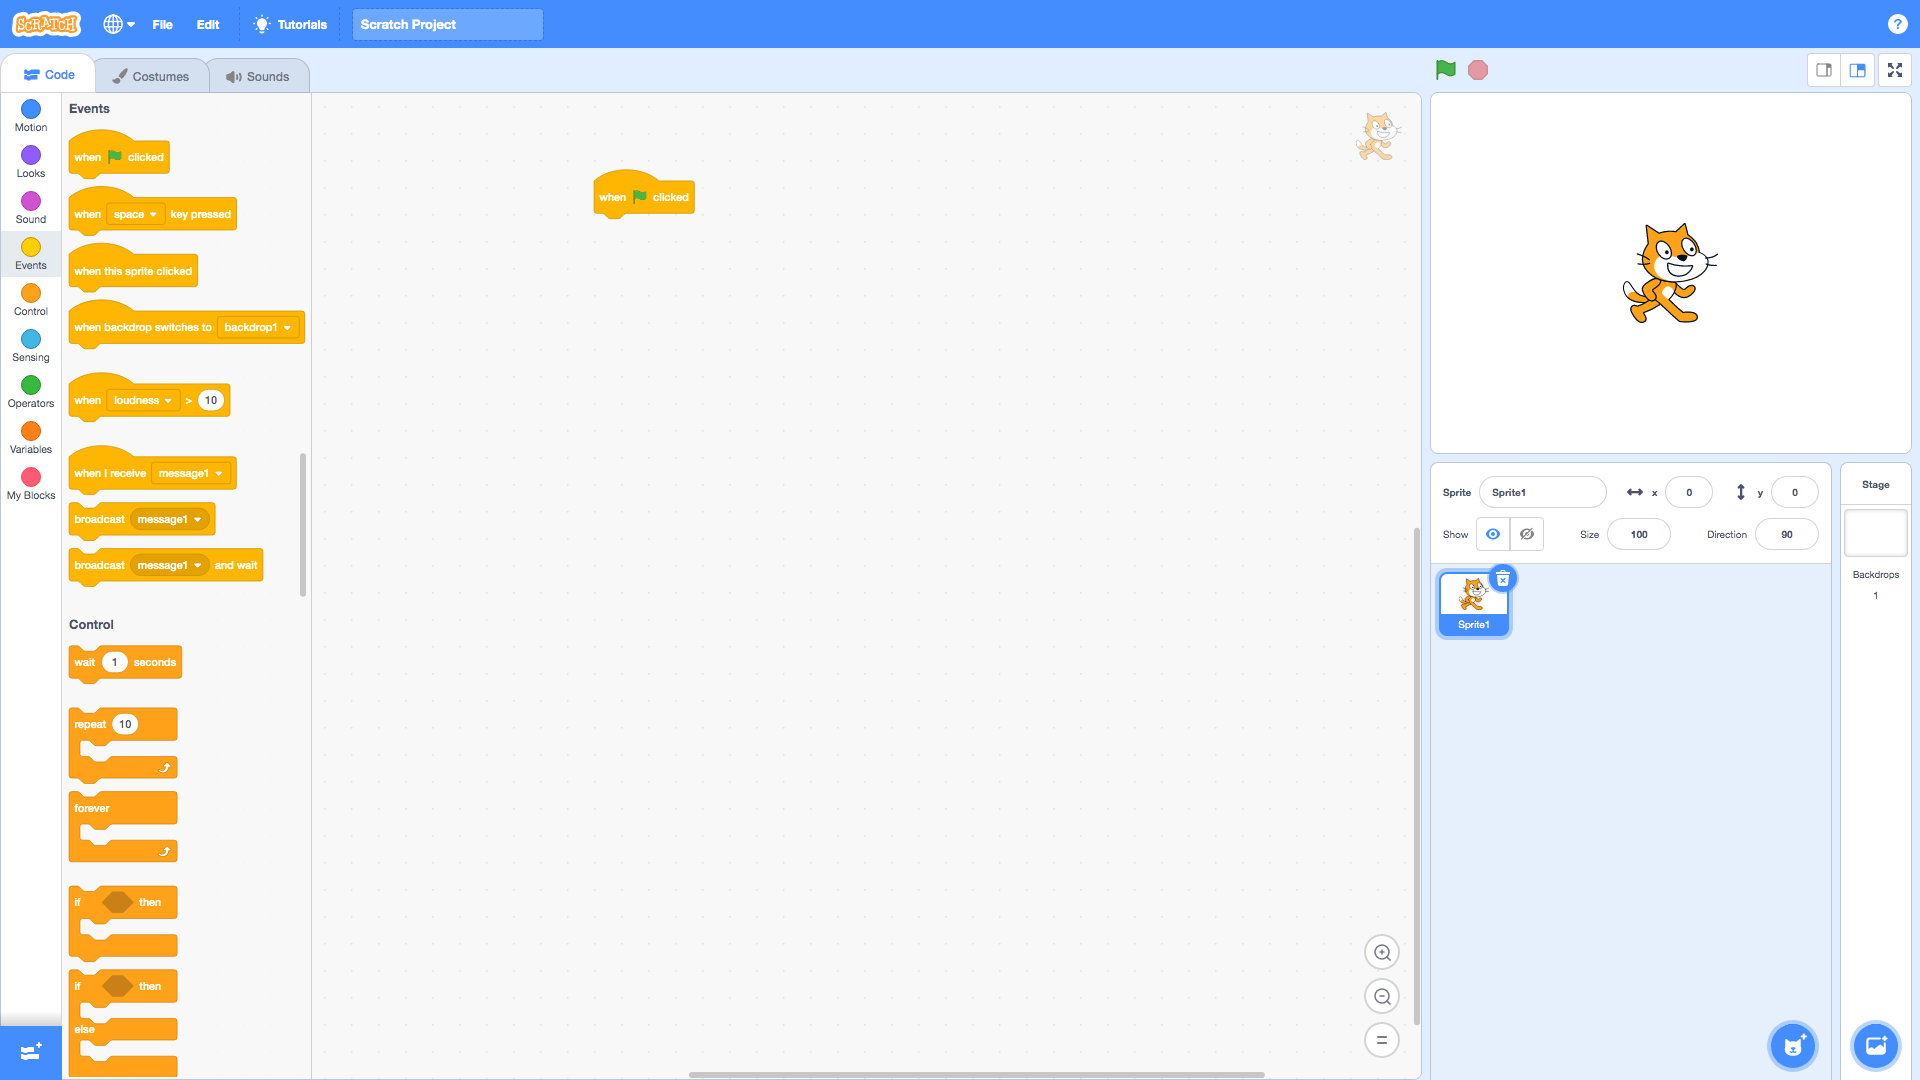
\includegraphics[width=1.0\linewidth,height=0.5\linewidth]{fig0052.png}
  \caption{Начална точка на програмата}
\label{fig0052}
\end{figure}

Блокчето за старт на програмата се намира в светло оранжевата група, която е предназначена да реагира на събития от страна на потребителя. Точният момент в който потребителят иска програмата да започне своето изпълнение е неопределен във времето и поради тази причина Scratch трябва да улови събитие, предизвикано от самия потребител. 

Второто по важност блокче служи за край на програмата (Фиг. \ref{fig0053}). То се намира в тъмно оранжевата група и има за задача да спре всички процеси, извършващи се по време на изпълнението на самата програма.

\begin{figure}[H]
  \centering
  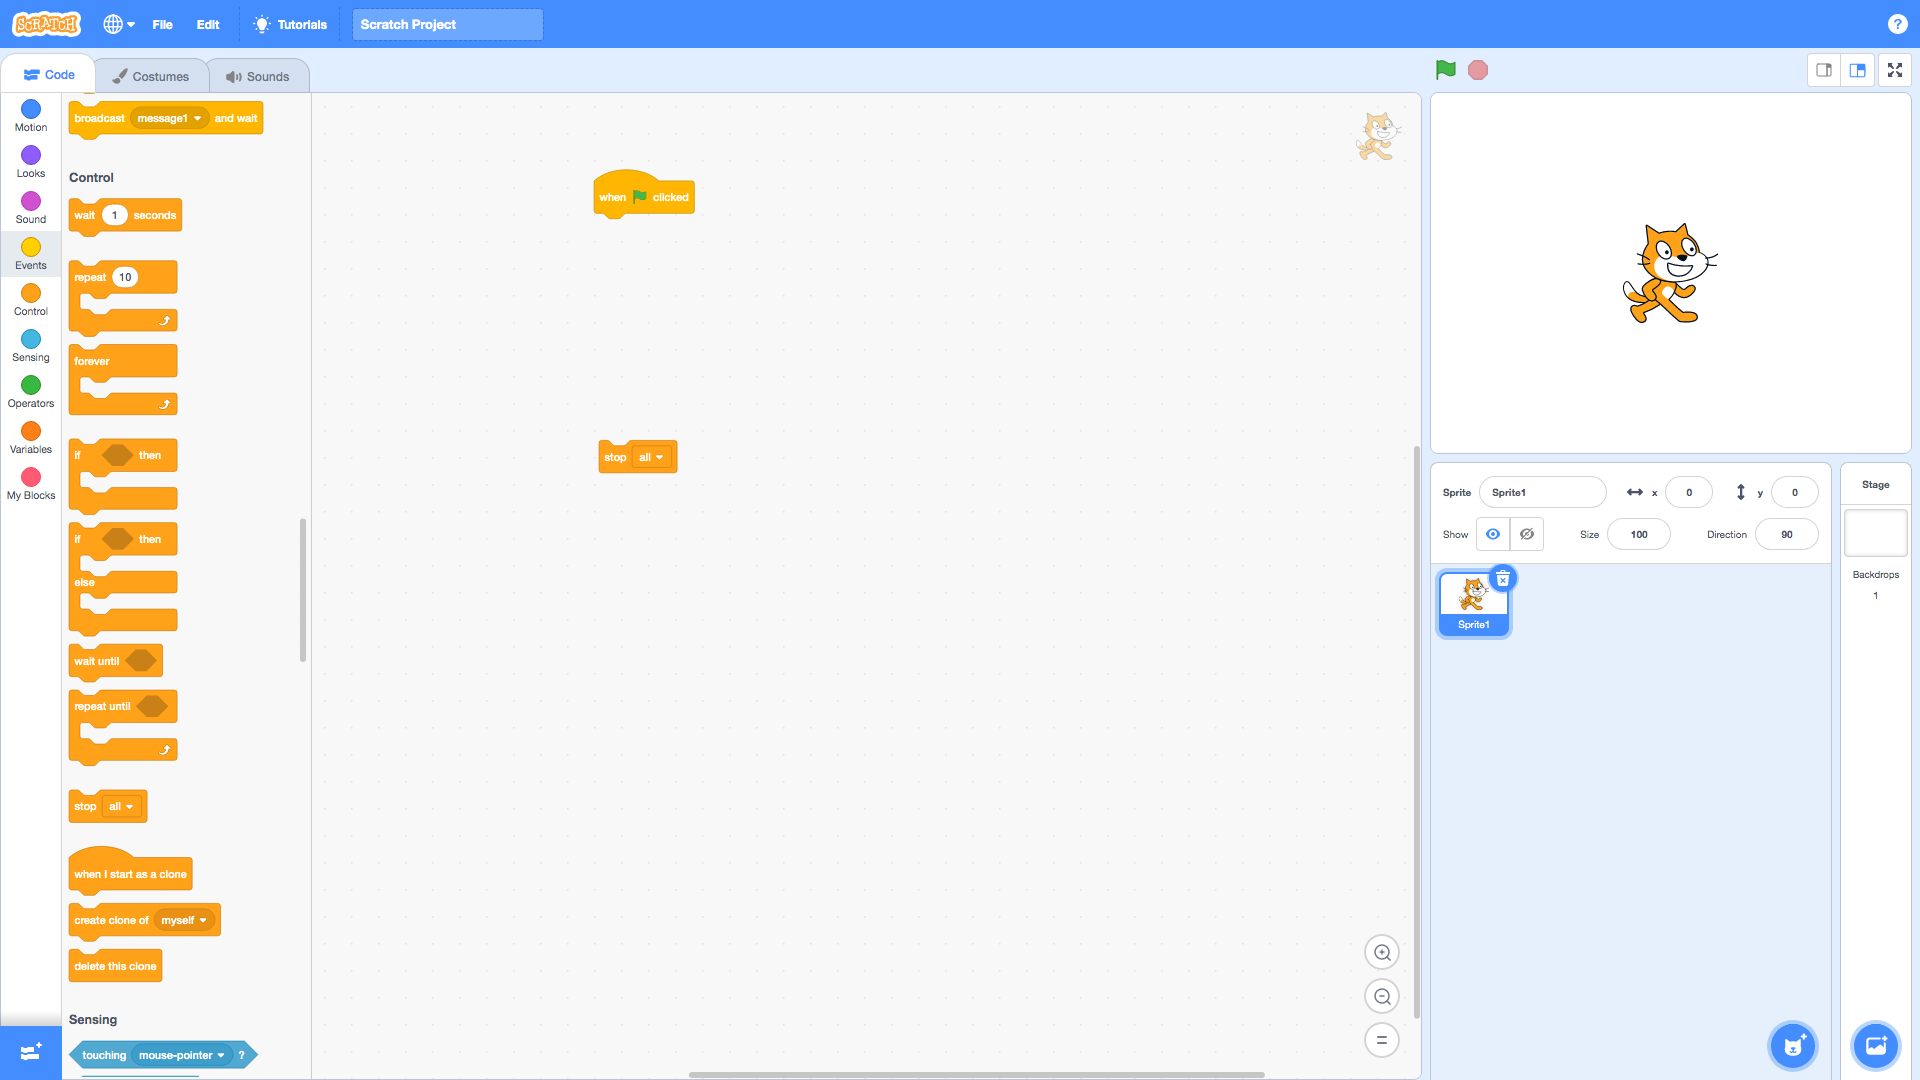
\includegraphics[width=1.0\linewidth,height=0.5\linewidth]{fig0053.png}
  \caption{Крайна точка на програмата}
\label{fig0053}
\end{figure}

Тъмно оранжевата група съдържа блокчета за контрол на изпълнението. Тези блокчета позволяват програмата да поема по различни пътища, както и група от действия да се повтарят многократно. 

В Scratch блокчетата инструкции основно контролират картинки, наречени спрайтове (sprites). За разлика от обикновеното компютърно изображение, спрайтът е графичен обект, който съдържа множество кадри, показващи изображението на героя в различни конфигурации. Всяка нова програма в Scratch започва с един спрайт, на оранжевата котка, разположена на координати (x=0,y=0). Работното пространство е двуизмерна координатна система с център (0,0). 

\begin{figure}[H]
  \centering
  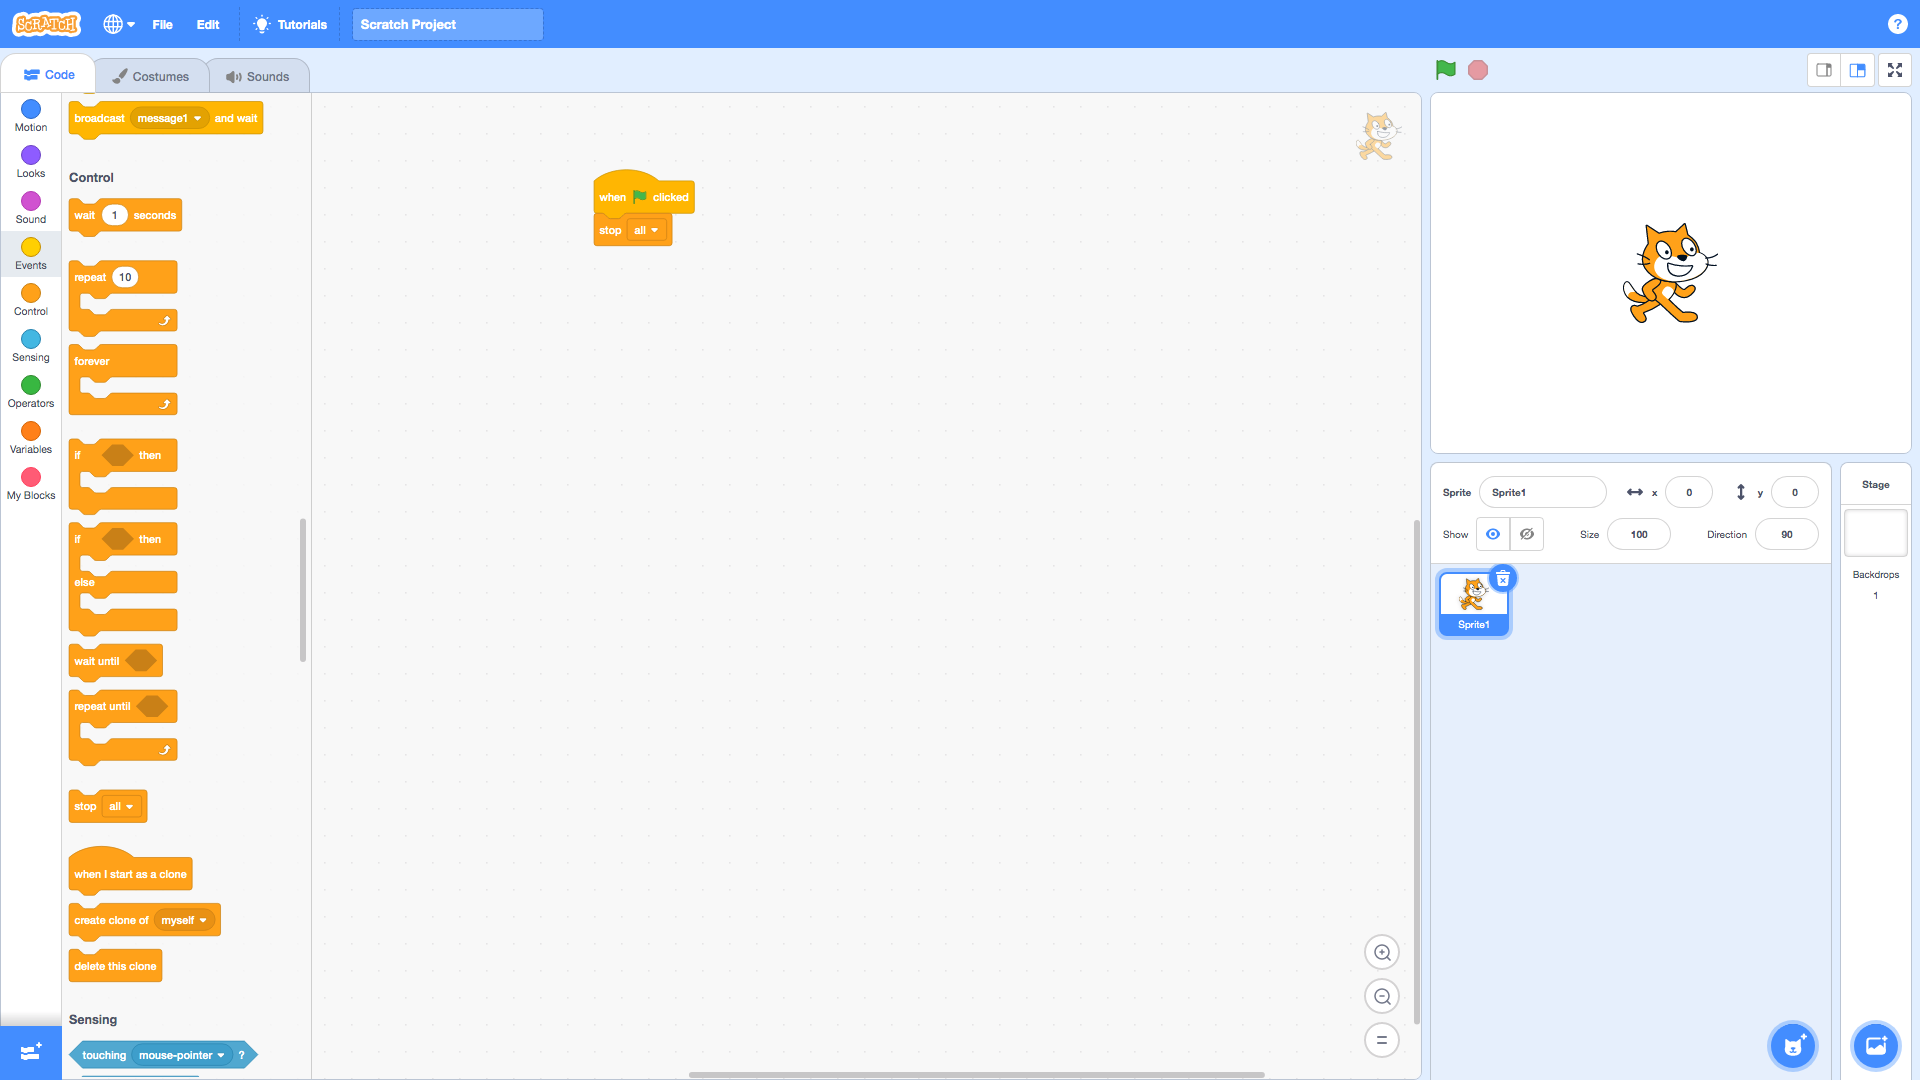
\includegraphics[width=1.0\linewidth,height=0.5\linewidth]{fig0054.png}
  \caption{Завършване веднага след започване}
\label{fig0054}
\end{figure}

Ако бъдат съединени, блокчетата за начало и за край (Фиг. \ref{fig0054}), то програмата не изпълнява нищо. Практически, тази програма приключва веднага след като е започнала. Програма, която не прави нищо е напълно безсмислена. За да започне нещо да се случва се използват блокчетата в синята група. Първото блокче инструктира котето да се премести 10 стъпки, като броя стъпки може да бъде променени, чрез изписване на друго число във вътрешността на блокчето (Фиг. \ref{fig0055}).

\begin{figure}[H]
  \centering
  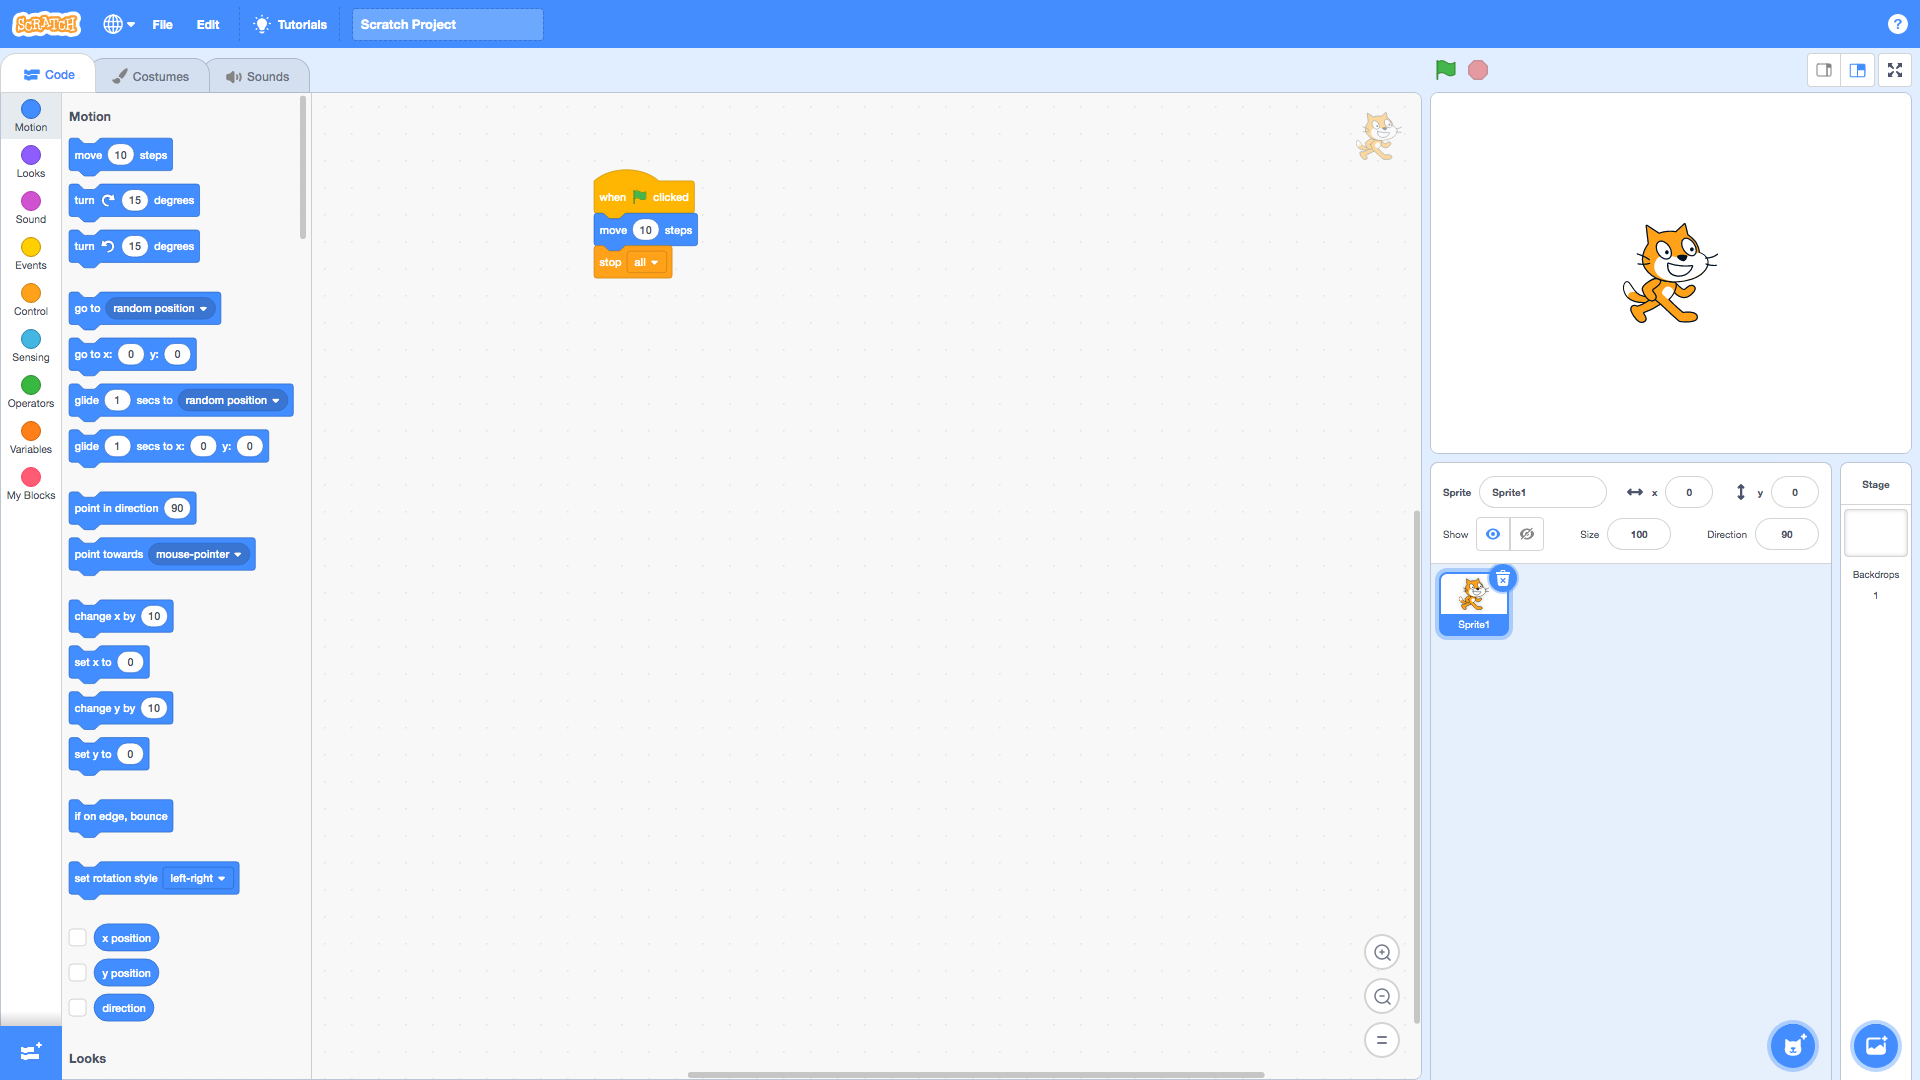
\includegraphics[width=1.0\linewidth,height=0.5\linewidth]{fig0055.png}
  \caption{Преместване на героя}
\label{fig0055}
\end{figure}

Следващият блок в групата инструктира героя да се завърти на определено число градуси, по часовниковата стрелка, спрямо собствения си център (Фиг. \ref{fig0056}).

\begin{figure}[H]
  \centering
  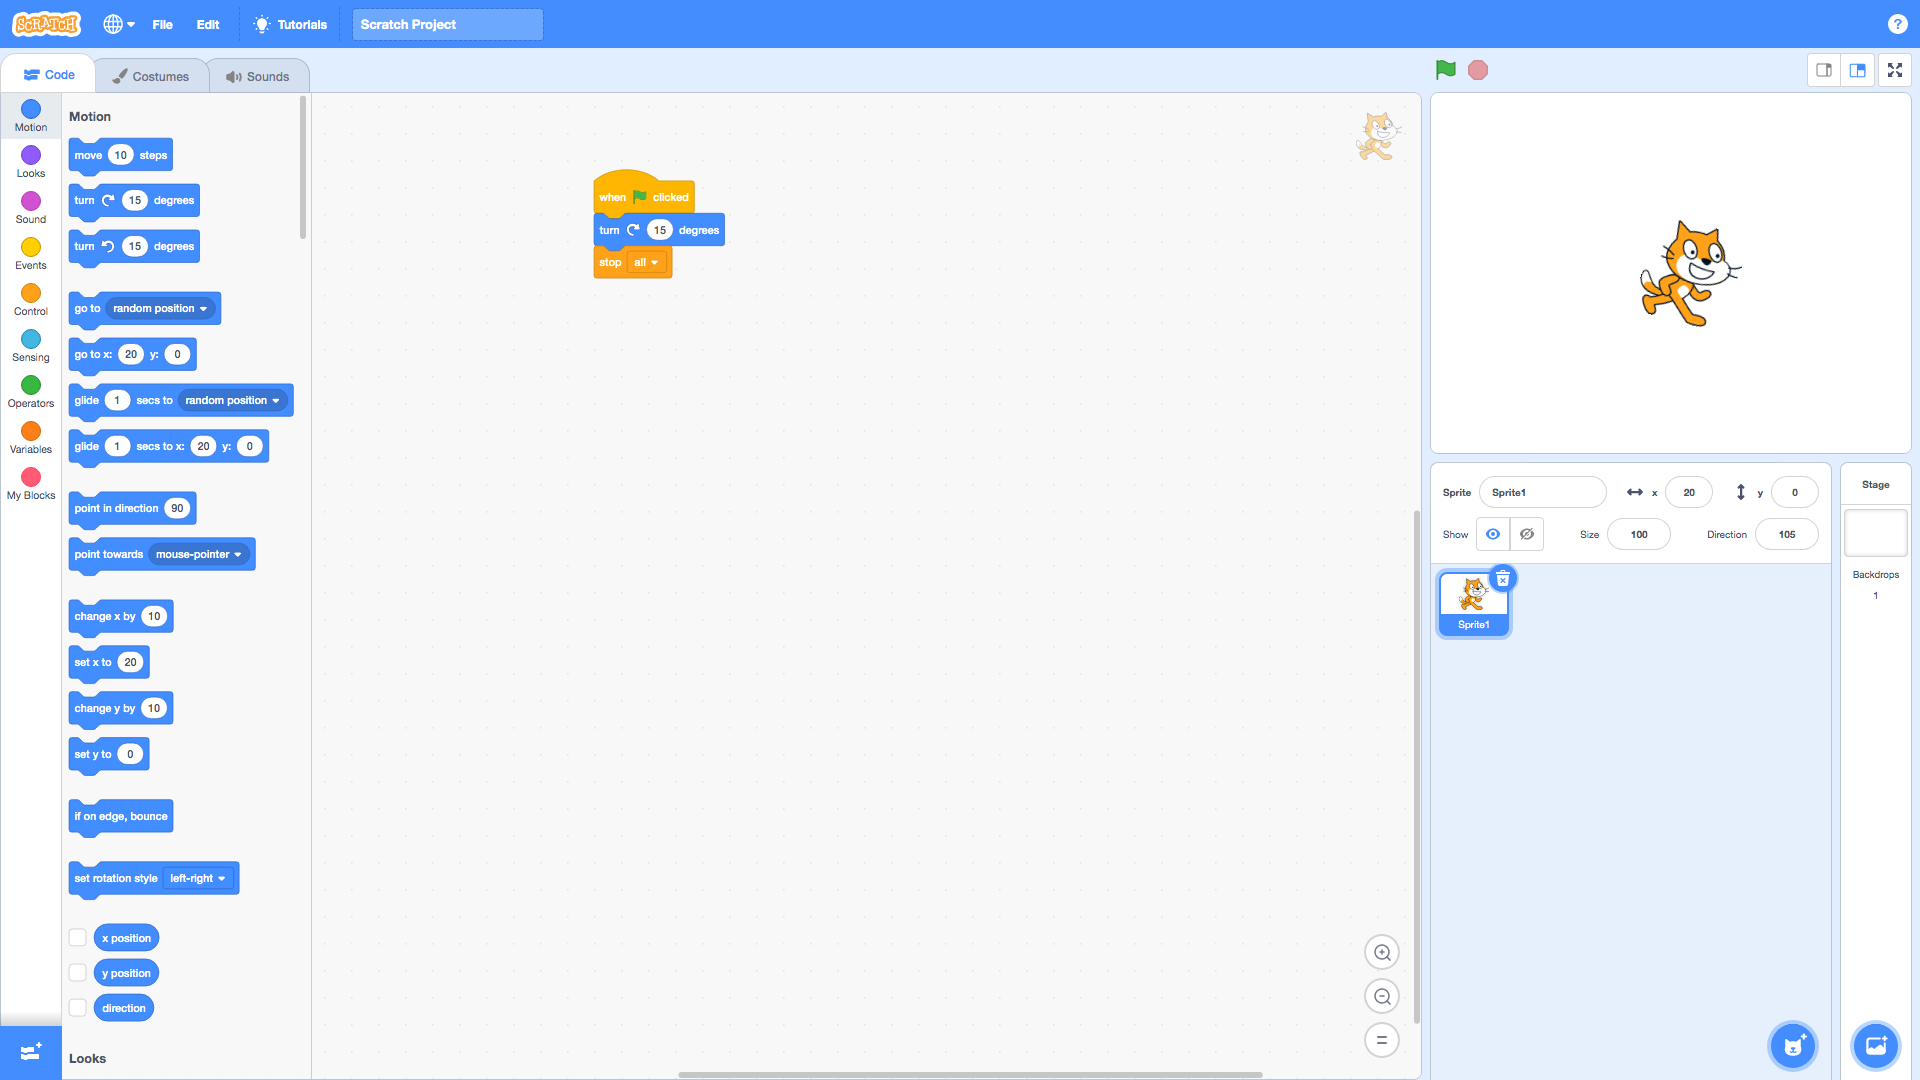
\includegraphics[width=1.0\linewidth,height=0.5\linewidth]{fig0056.png}
  \caption{Завъртане по часовниковата стрелка}
\label{fig0056}
\end{figure}

Аналогично, със следващото блокче в групата, завъртането може да се изпълни и в посока обратна на часовниковата стрелка (Фиг. \ref{fig0057}).

\begin{figure}[H]
  \centering
  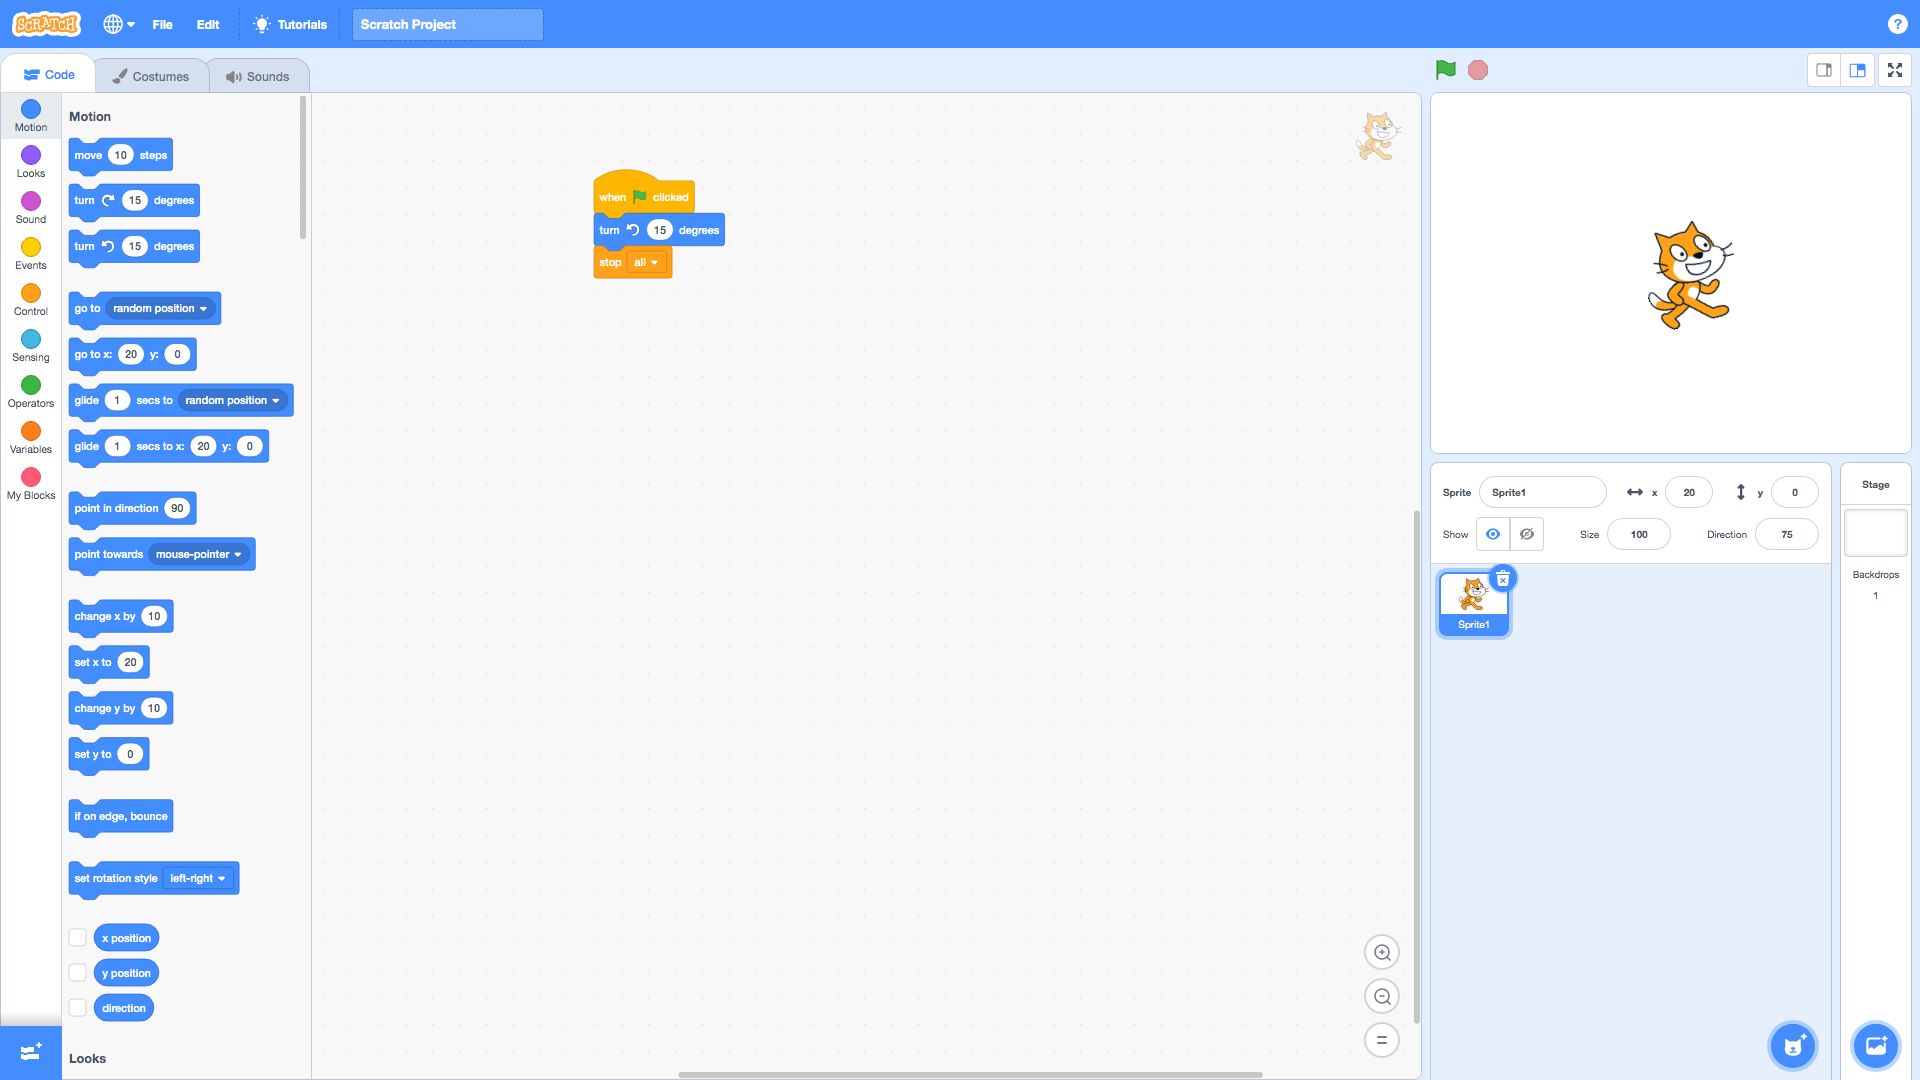
\includegraphics[width=1.0\linewidth,height=0.5\linewidth]{fig0057.png}
  \caption{Завъртане обратно на часовниковата стрелка}
\label{fig0057}
\end{figure}

Следващия блок в групата дава възможност героят да се премести на случайни координати или на координати посочени с мишката (Фиг. \ref{fig0058}).

\begin{figure}[H]
  \centering
  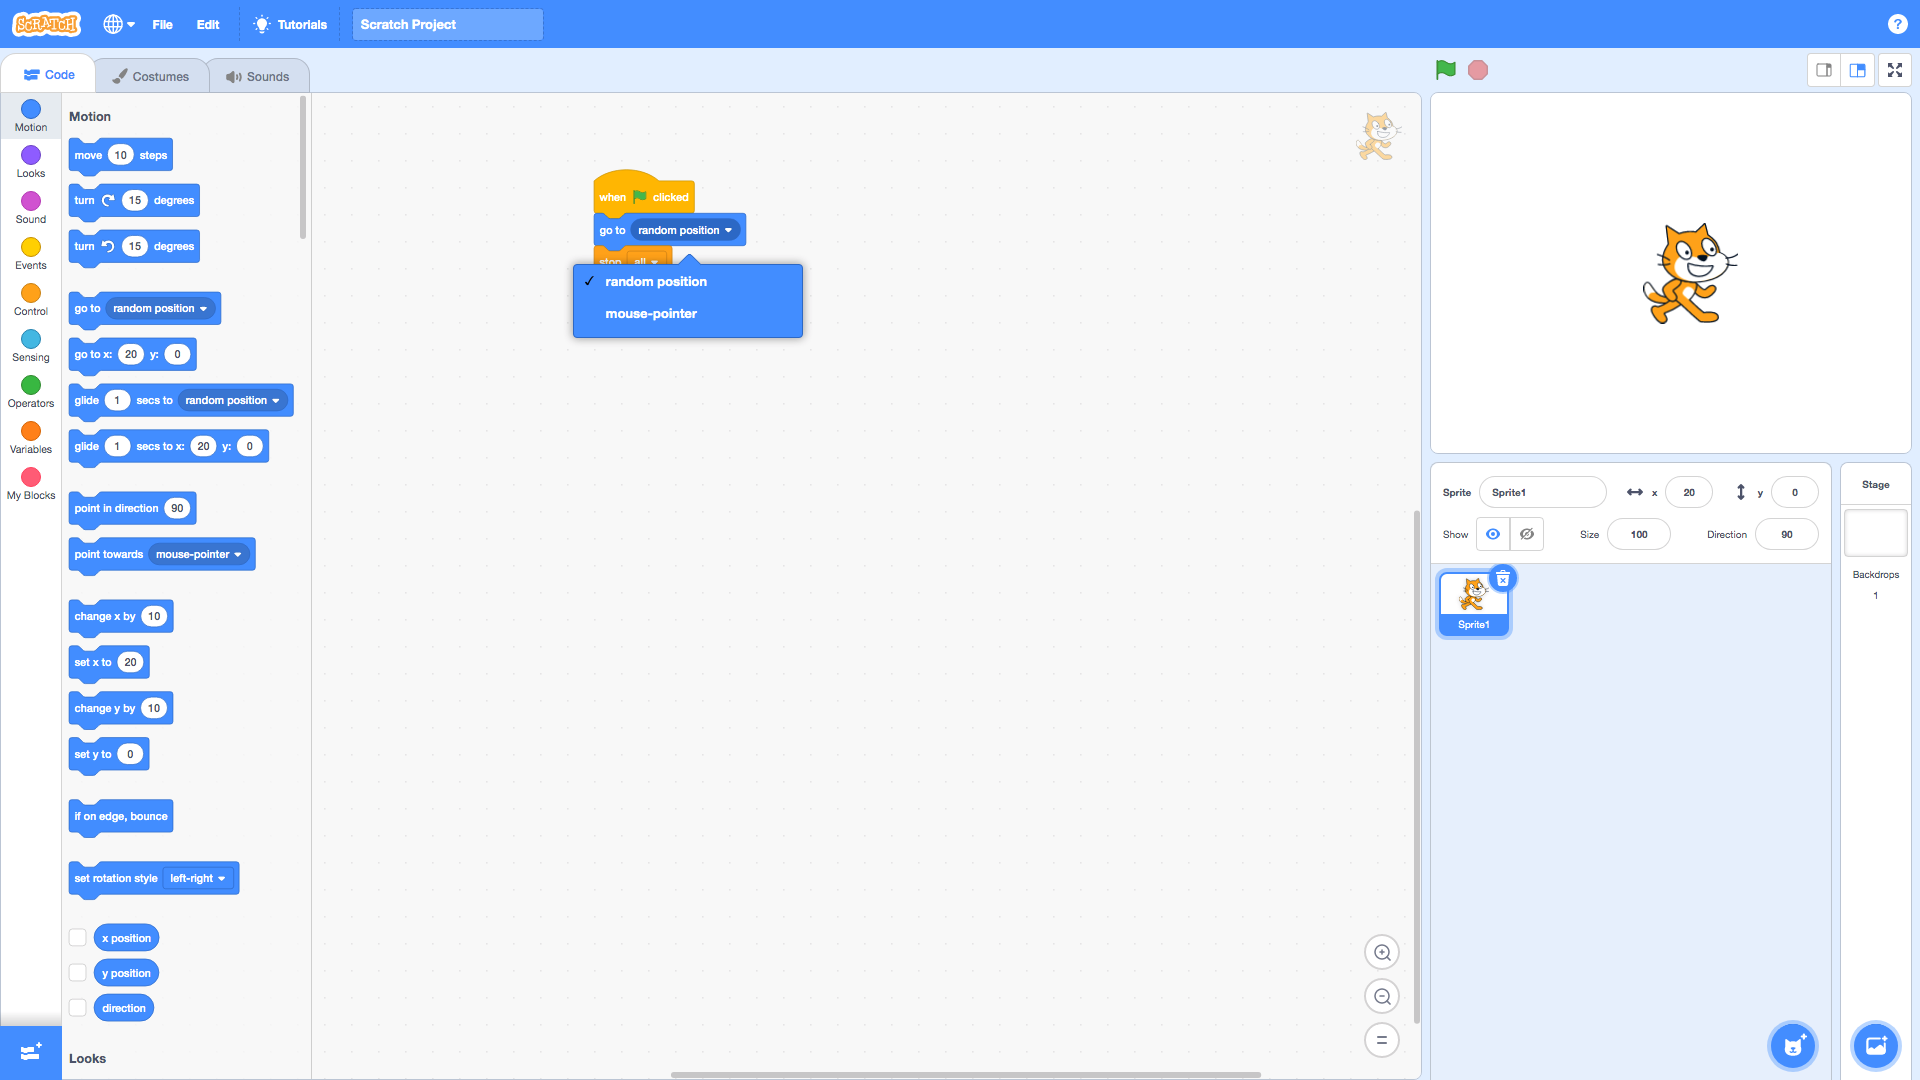
\includegraphics[width=1.0\linewidth,height=0.5\linewidth]{fig0058.png}
  \caption{Преместване на случайна позиция}
\label{fig0058}
\end{figure}

Движението на героя може да бъде зададено и чрез абсолютни координати с блокче, позволяващо да се впишат числа за абцисната и ординатната ос (Фиг. \ref{fig0059}).

\begin{figure}[H]
  \centering
  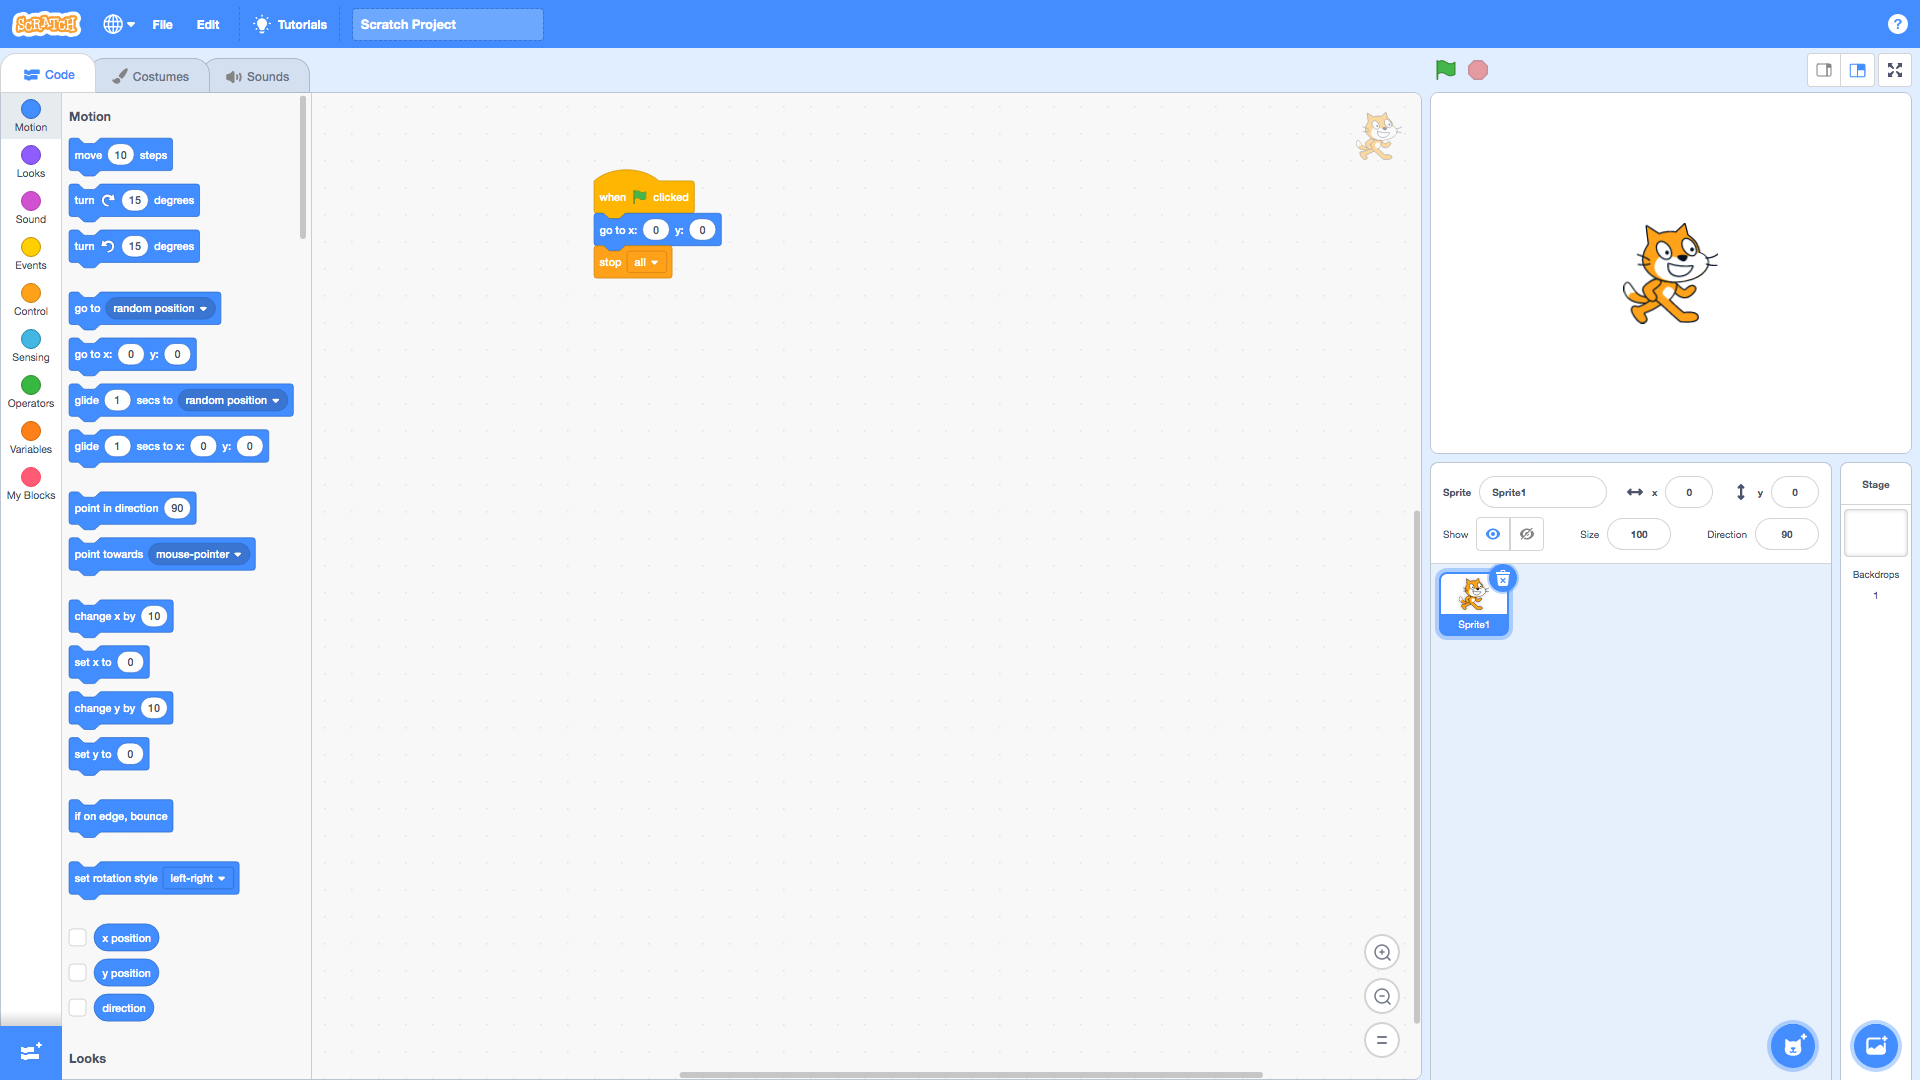
\includegraphics[width=1.0\linewidth,height=0.5\linewidth]{fig0059.png}
  \caption{Преместване по абсолютни координати}
\label{fig0059}
\end{figure}

Плавно придвижване, по предварително зададен интервал от време, е възможно на случайни координати или координати посочени с мишката, благодарение на следващото блокче в групата (Фиг. \ref{fig0060}).

\begin{figure}[H]
  \centering
  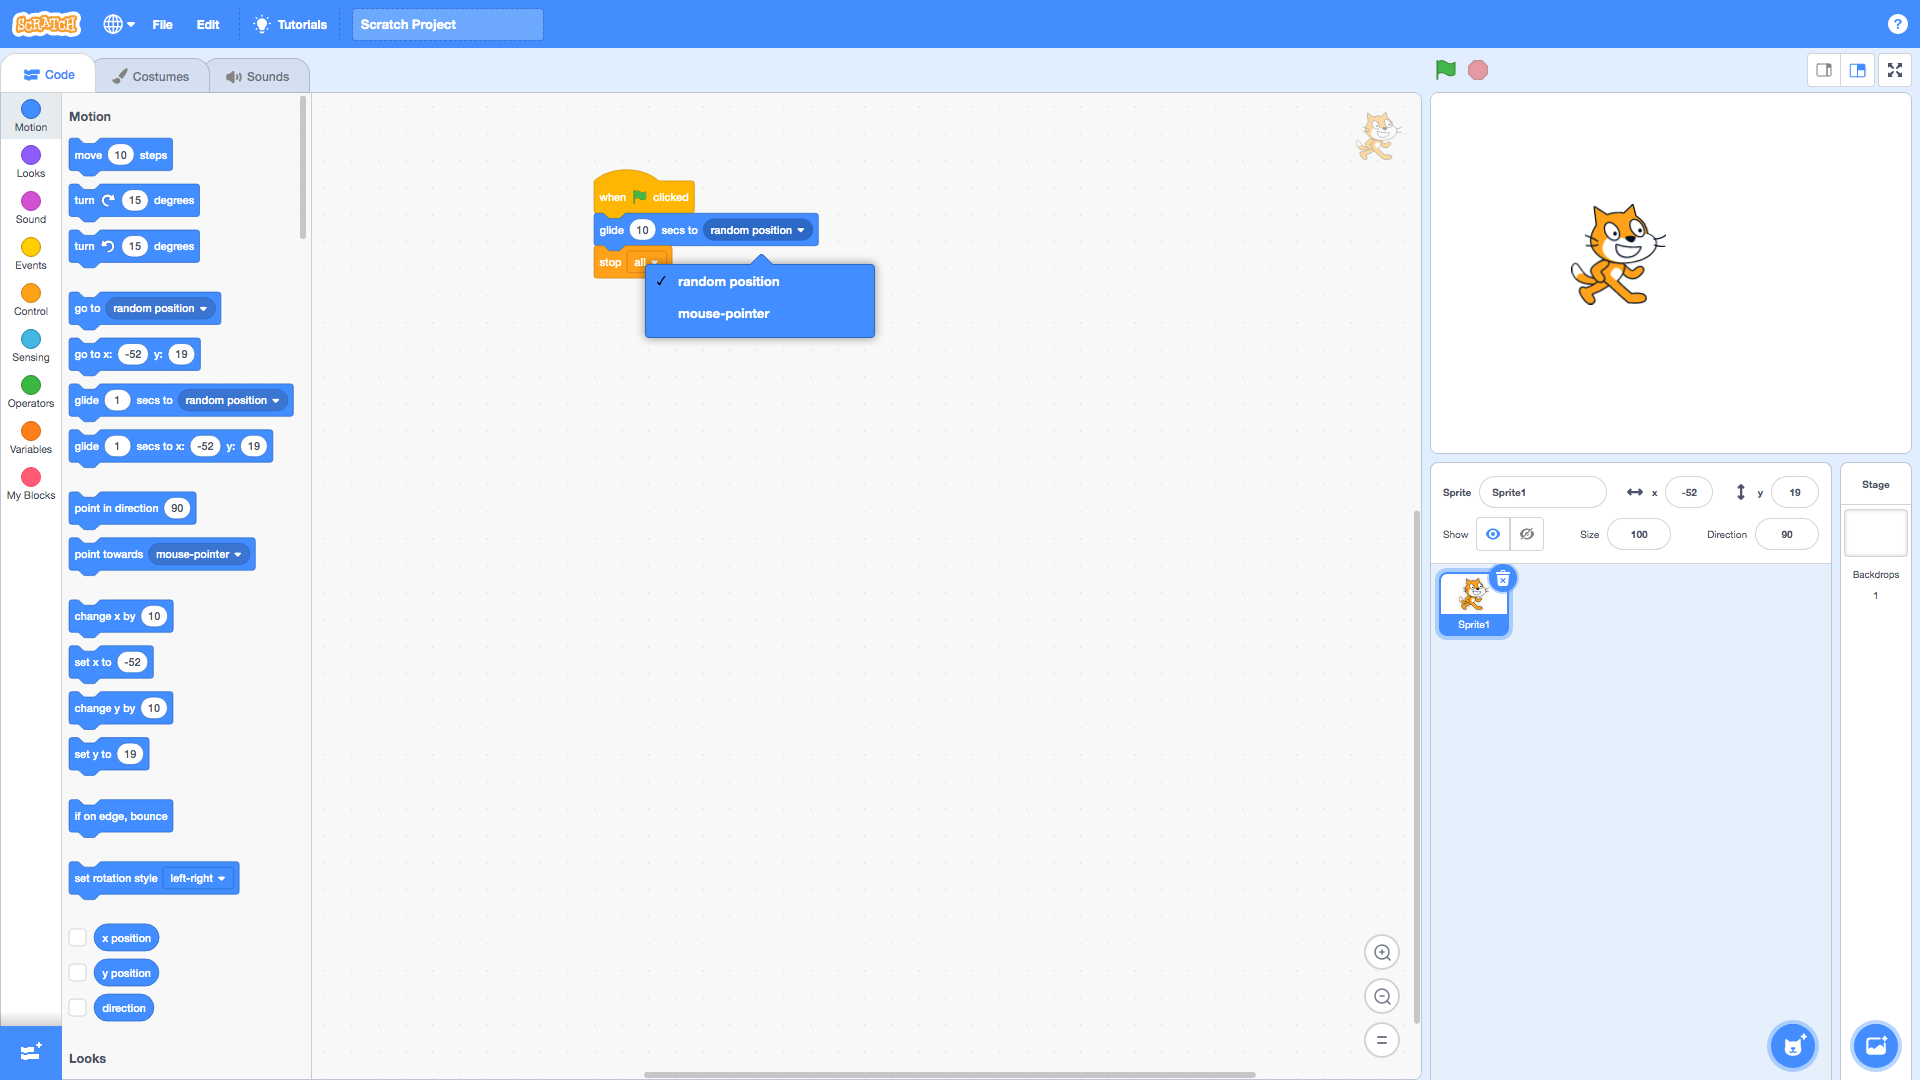
\includegraphics[width=1.0\linewidth,height=0.5\linewidth]{fig0060.png}
  \caption{Плъзгане до случайна позиция}
\label{fig0060}
\end{figure}

Плавното плъзгане до предварително зададени координати, за предварително определен интервал от време, е възможно с блокчето предназначено за тази цел (Фиг. \ref{fig0061}).

\begin{figure}[H]
  \centering
  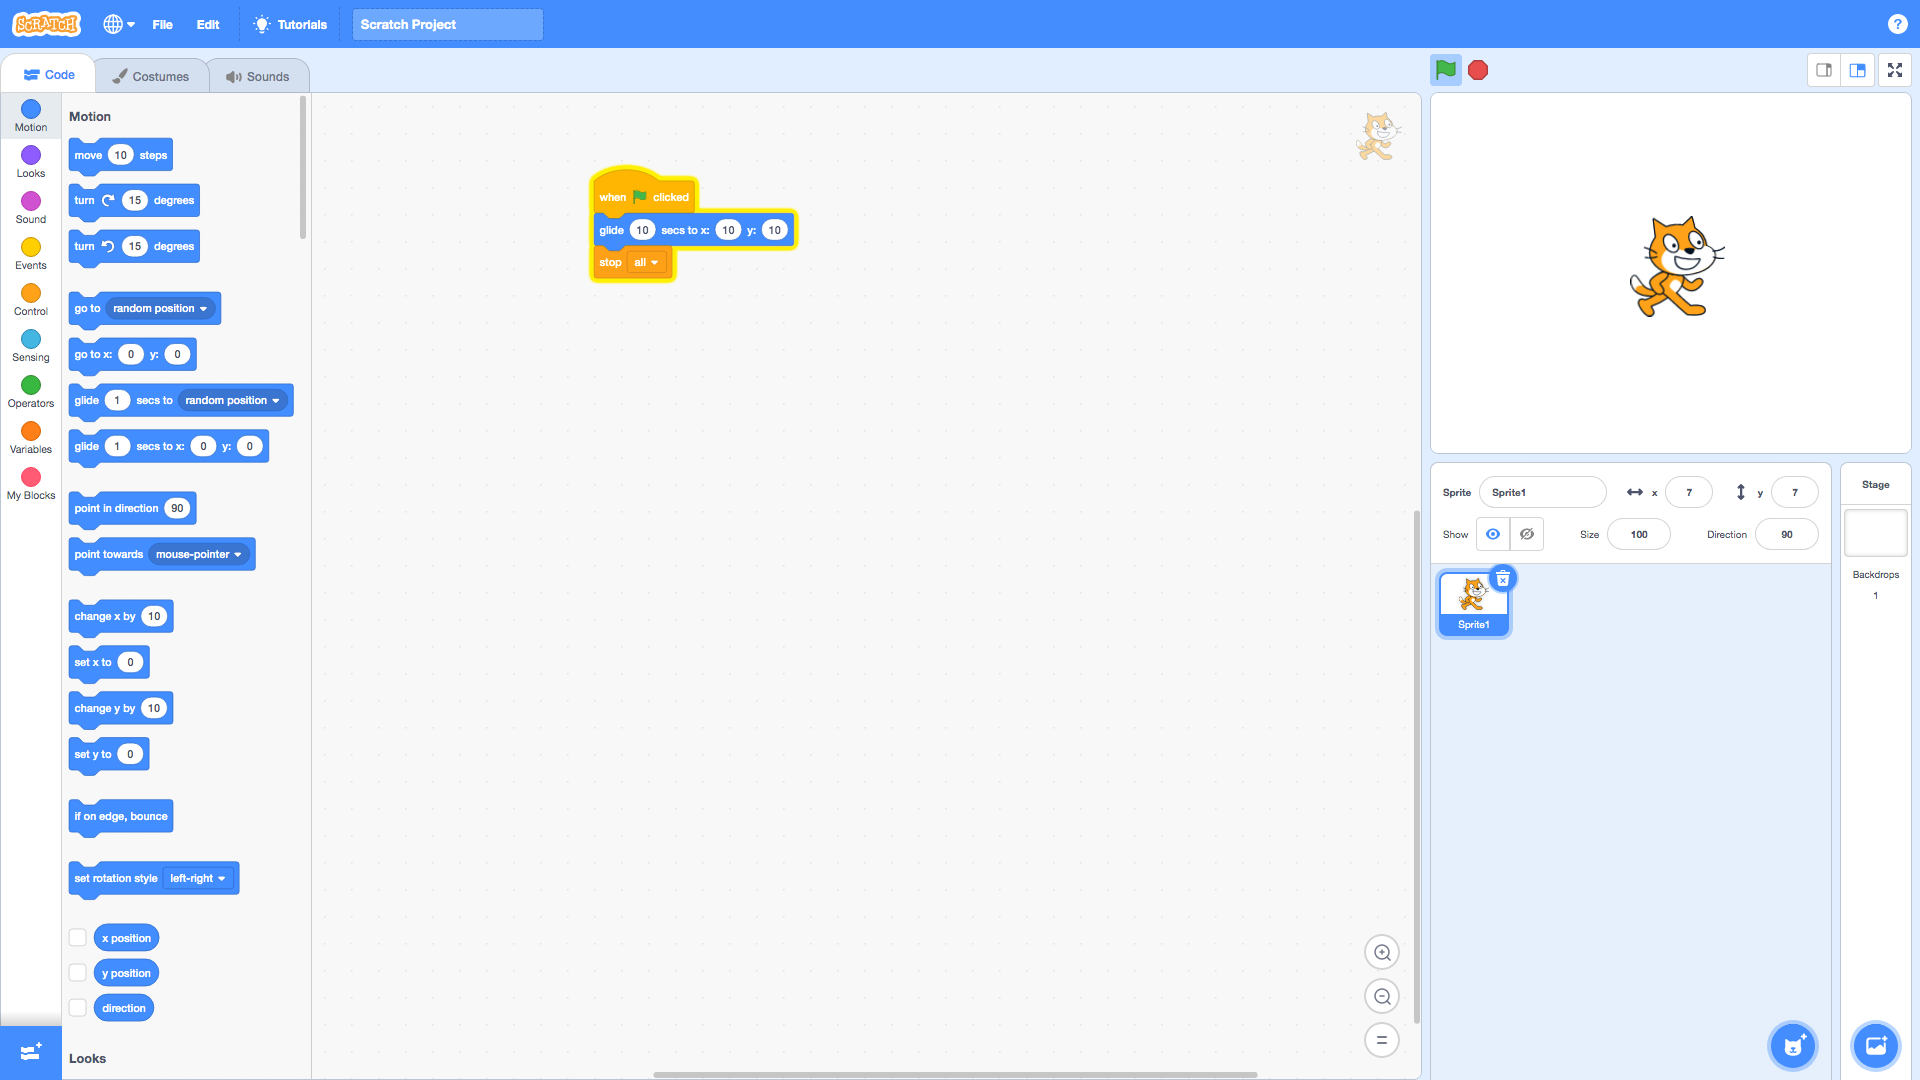
\includegraphics[width=1.0\linewidth,height=0.5\linewidth]{fig0061.png}
  \caption{Плъзгане до зададени координати}
\label{fig0061}
\end{figure}

Анимираният герой има характеристика за ориентация, под формата на ъгъл. При 90 градуса, оранжевата котка гледа на дясно. За да се промени ориентацията на героя се използва блокче с възможност за въвеждане на конкретен ъгъл (Фиг. \ref{fig0062}).

\begin{figure}[H]
  \centering
  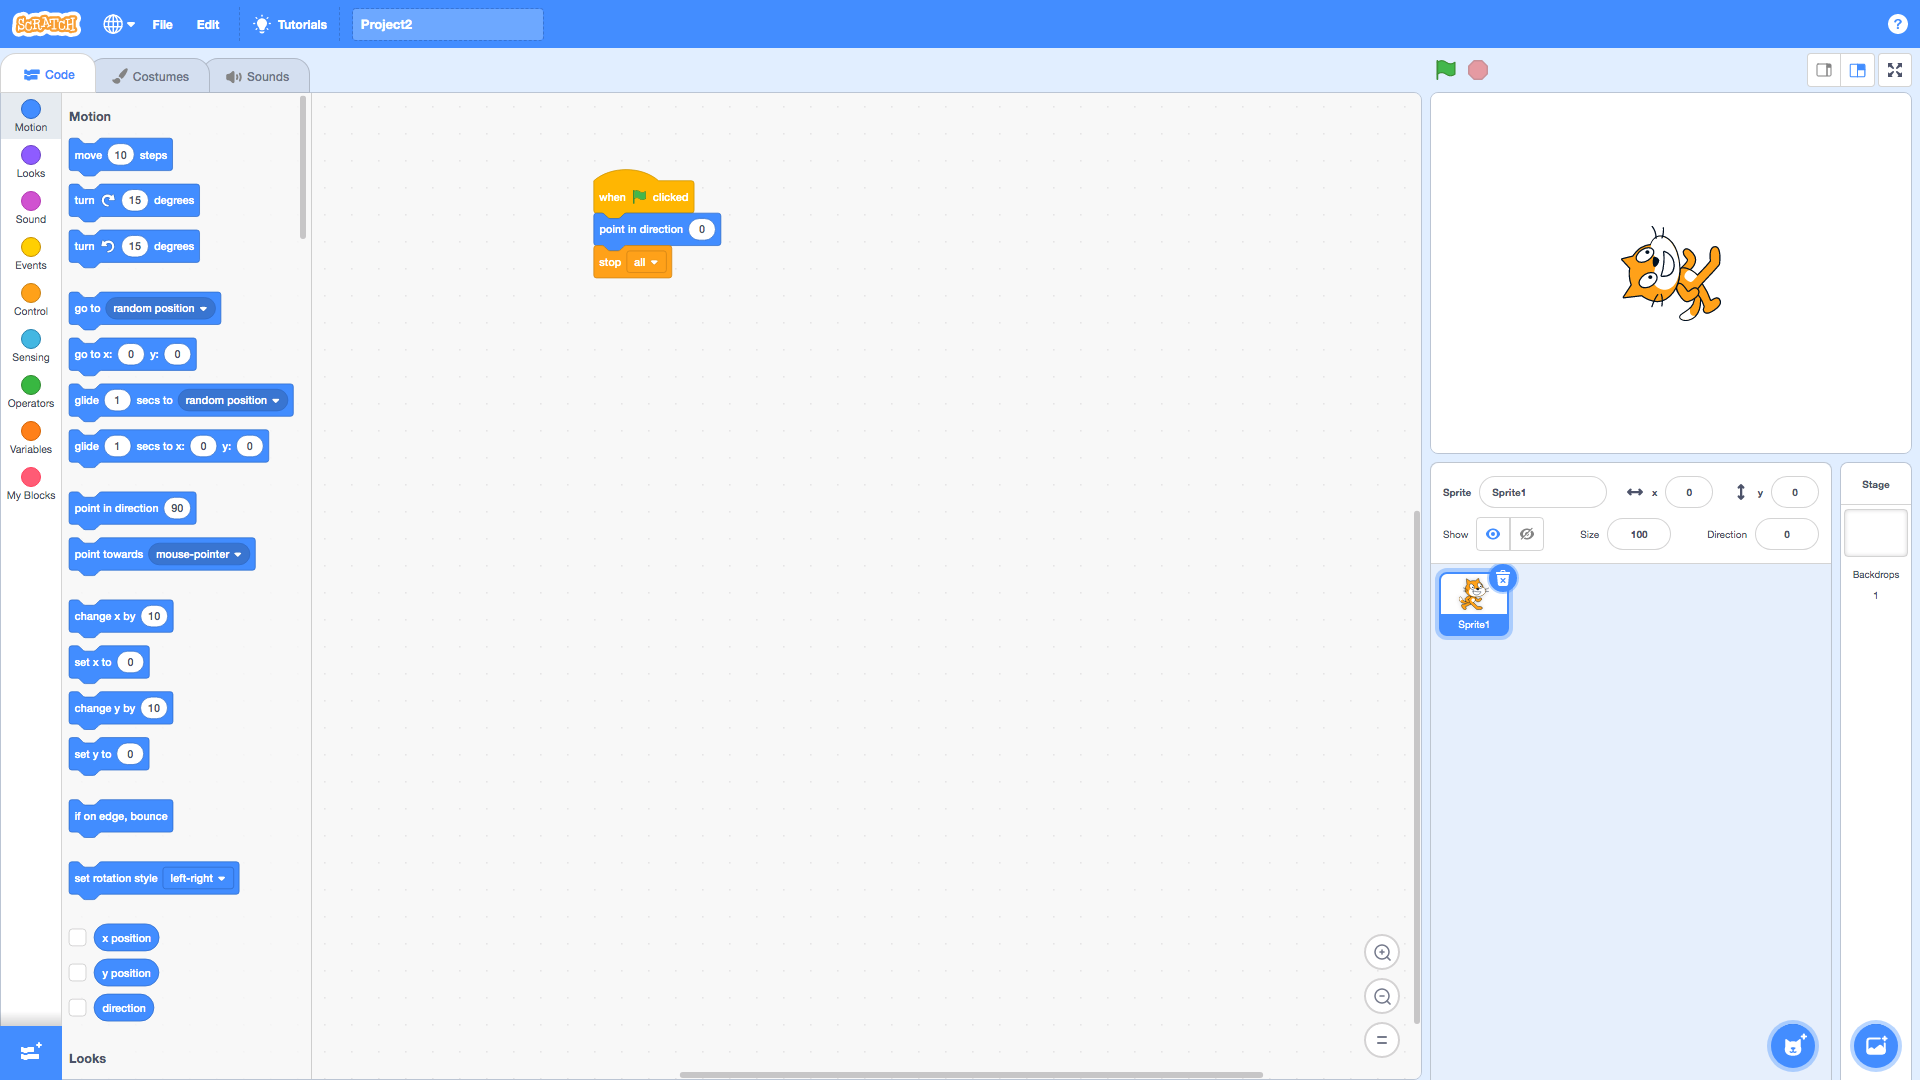
\includegraphics[width=1.0\linewidth,height=0.5\linewidth]{fig0062.png}
  \caption{Ъглова ориентация}
\label{fig0062}
\end{figure}

При по-сложни сценарии за управление на героя, понякога е нужно героят да следи показалеца на мишката. За тази цел има определено блокче, което изпълнява тази инструкция (Фиг. \ref{fig0063}).

\begin{figure}[H]
  \centering
  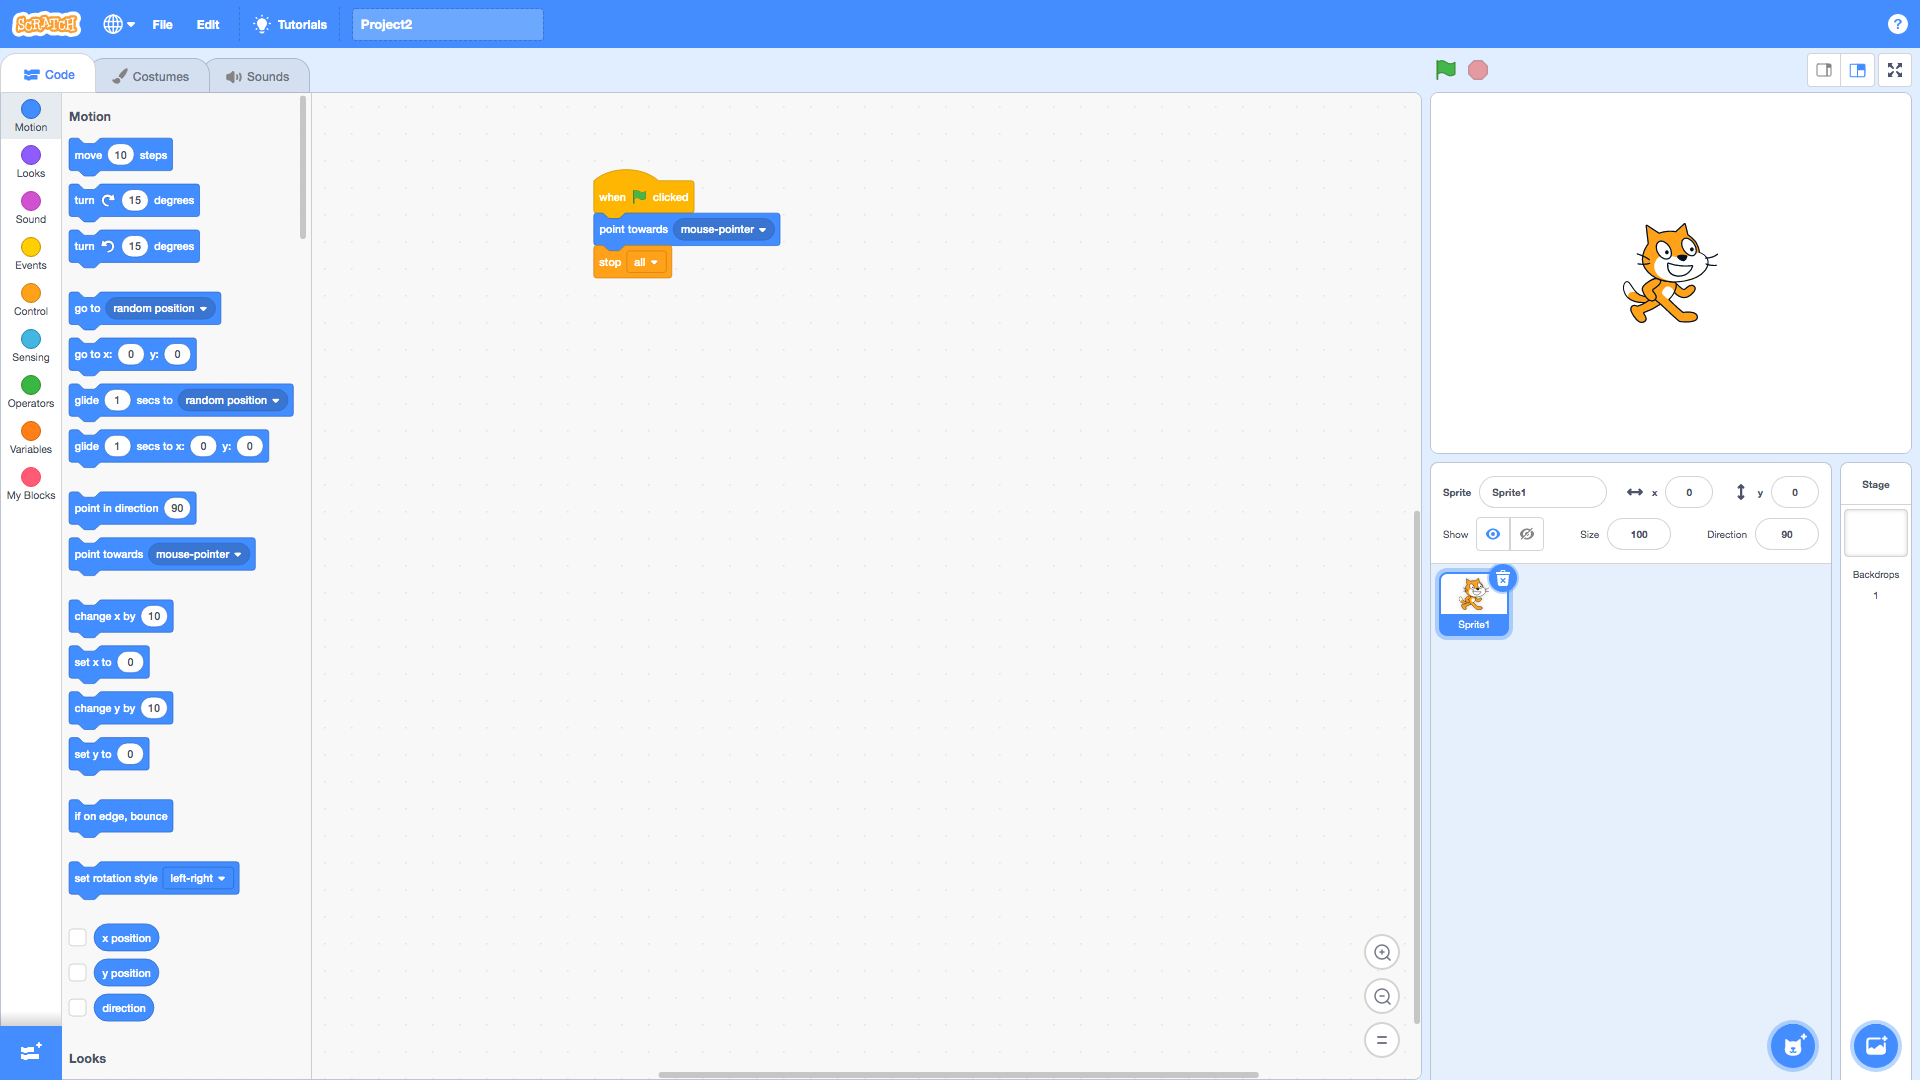
\includegraphics[width=1.0\linewidth,height=0.5\linewidth]{fig0063.png}
  \caption{Ориентация по показалеца на мишката}
\label{fig0063}
\end{figure}

Блокчетата могат да се поставят едно след друго, като за последователна промяна на относителните x и y координатите (относителни, спрямо текущата позиция) на героя има специално определени блокчета (Фиг. \ref{fig0064}).

\begin{figure}[H]
  \centering
  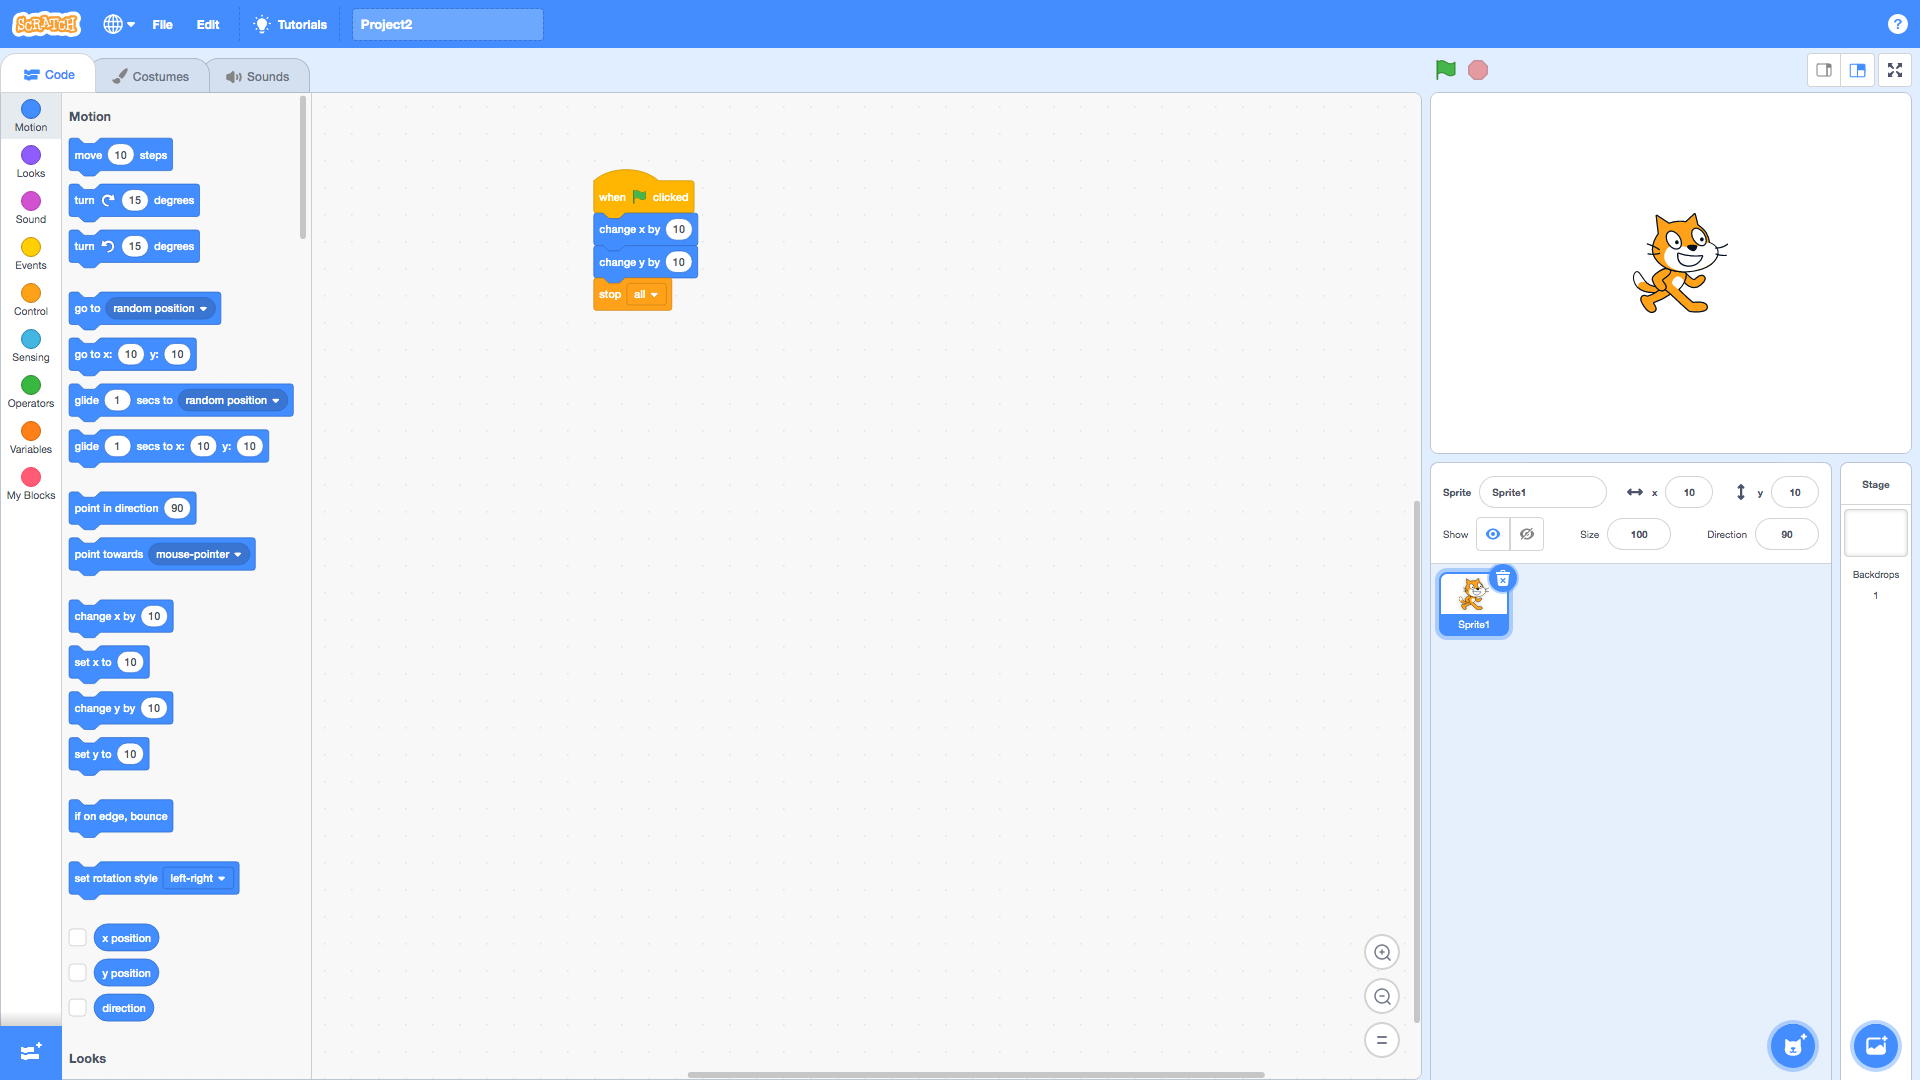
\includegraphics[width=1.0\linewidth,height=0.5\linewidth]{fig0064.png}
  \caption{Последователна промяна на относителни координати}
\label{fig0064}
\end{figure}

Освен относителна промяна на координатите е възможна и абсолютна промяна на координатите, като абсолютната промяна е спрямо центъра на координатната система (Фиг. \ref{fig0065}).

\begin{figure}[H]
  \centering
  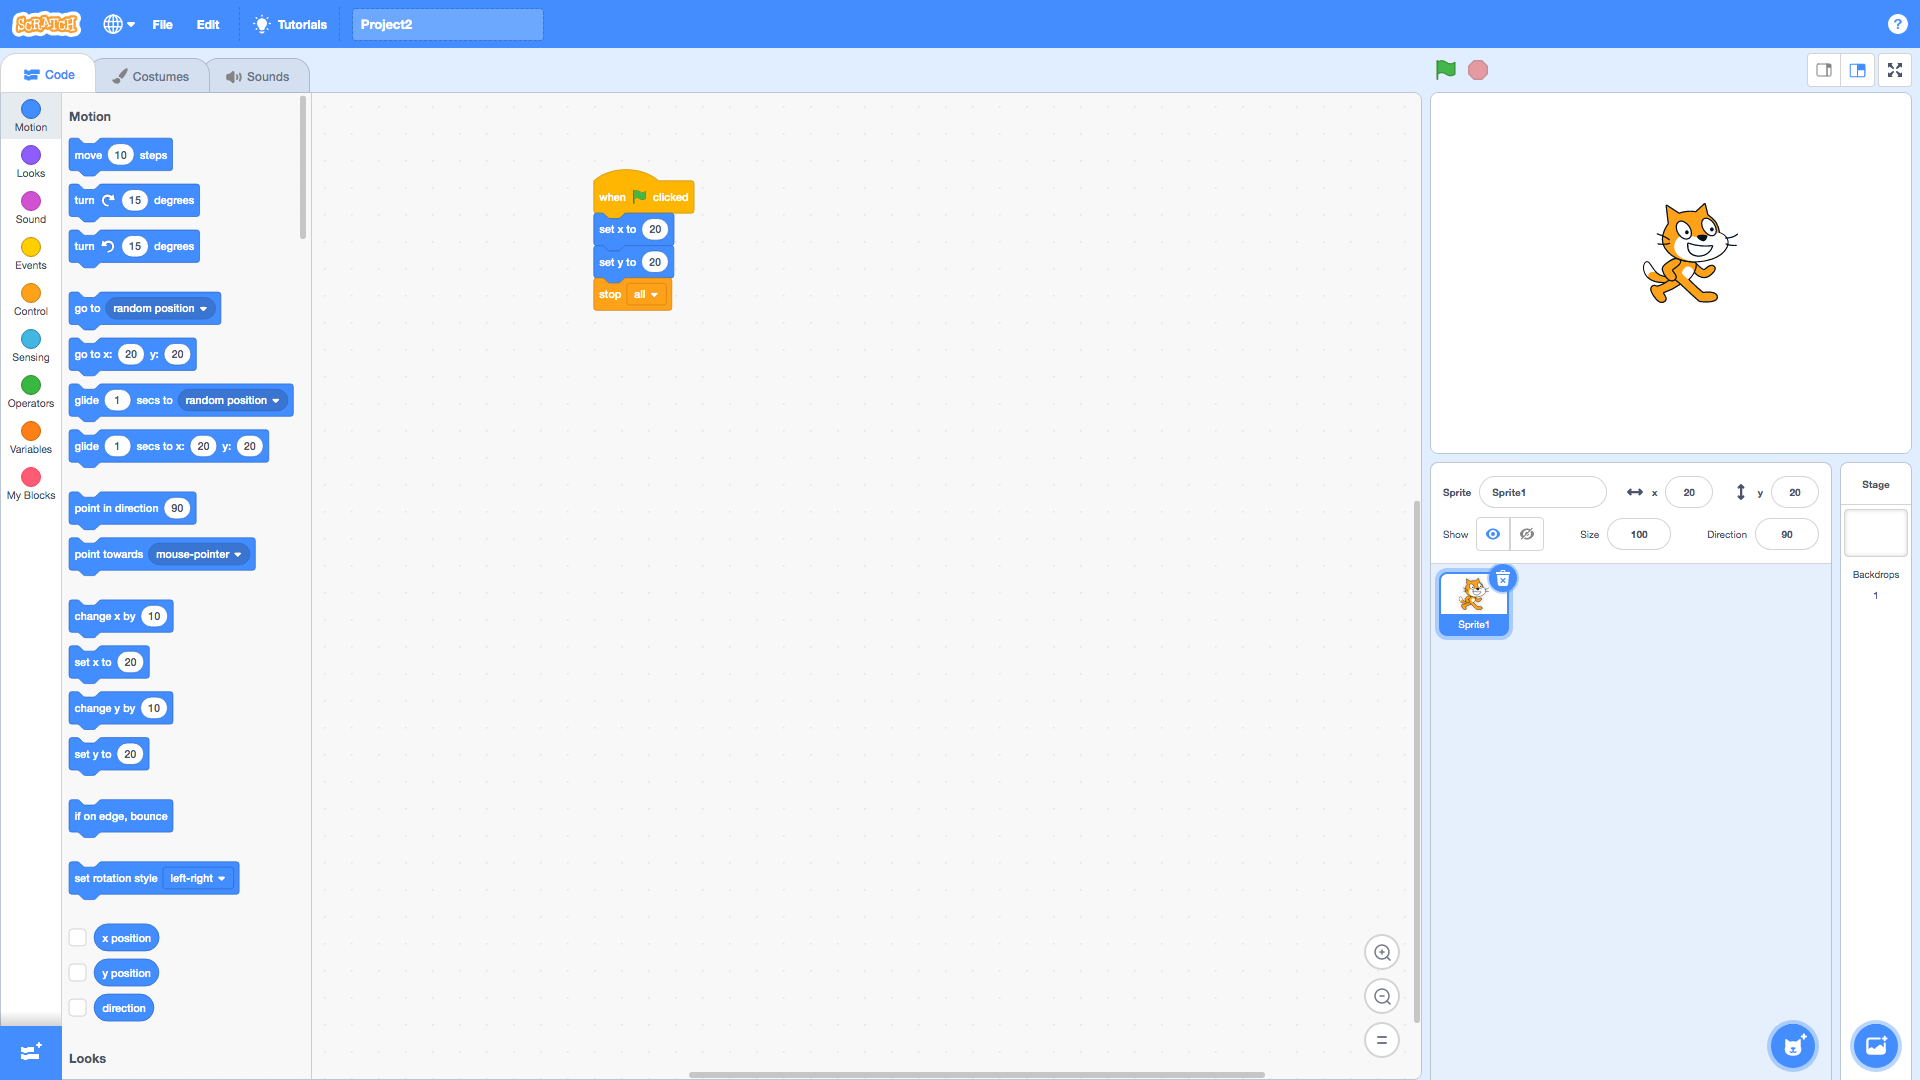
\includegraphics[width=1.0\linewidth,height=0.5\linewidth]{fig0065.png}
  \caption{Последователна промяна на абсолютни координати}
\label{fig0065}
\end{figure}

При своето движение, когато анимираният герой достигне границите на работното пространство, единият вариант е движението да продължи извън видимата зона. Другият вариант е да се вземат мерки и героят да отскача от ръбовете на работното пространство. За това отскачане има конкретно блокче (Фиг. \ref{fig0066}). За да се илюстрира работата му е нужна малко по-сложна последователност от инструкции. При всяко стартиране на програмата, първо се променят относителните координати, а след това се извършва отскачане от ръба, ако е необходимо. За да бъде малко по-интересен сценарият за проверка, вместо фиксирани стойности за относително отместване се използва вграждане на едно от зелените блокчета, което позволява генериране на случайно число в предварително определен диапазон. Съществено е да се забележи, че зеленото блокче има овална форма, което подсказва, че то е предназначено за вграждане в някой от другите блокове, които имат овален слот. 

\begin{figure}[H]
  \centering
  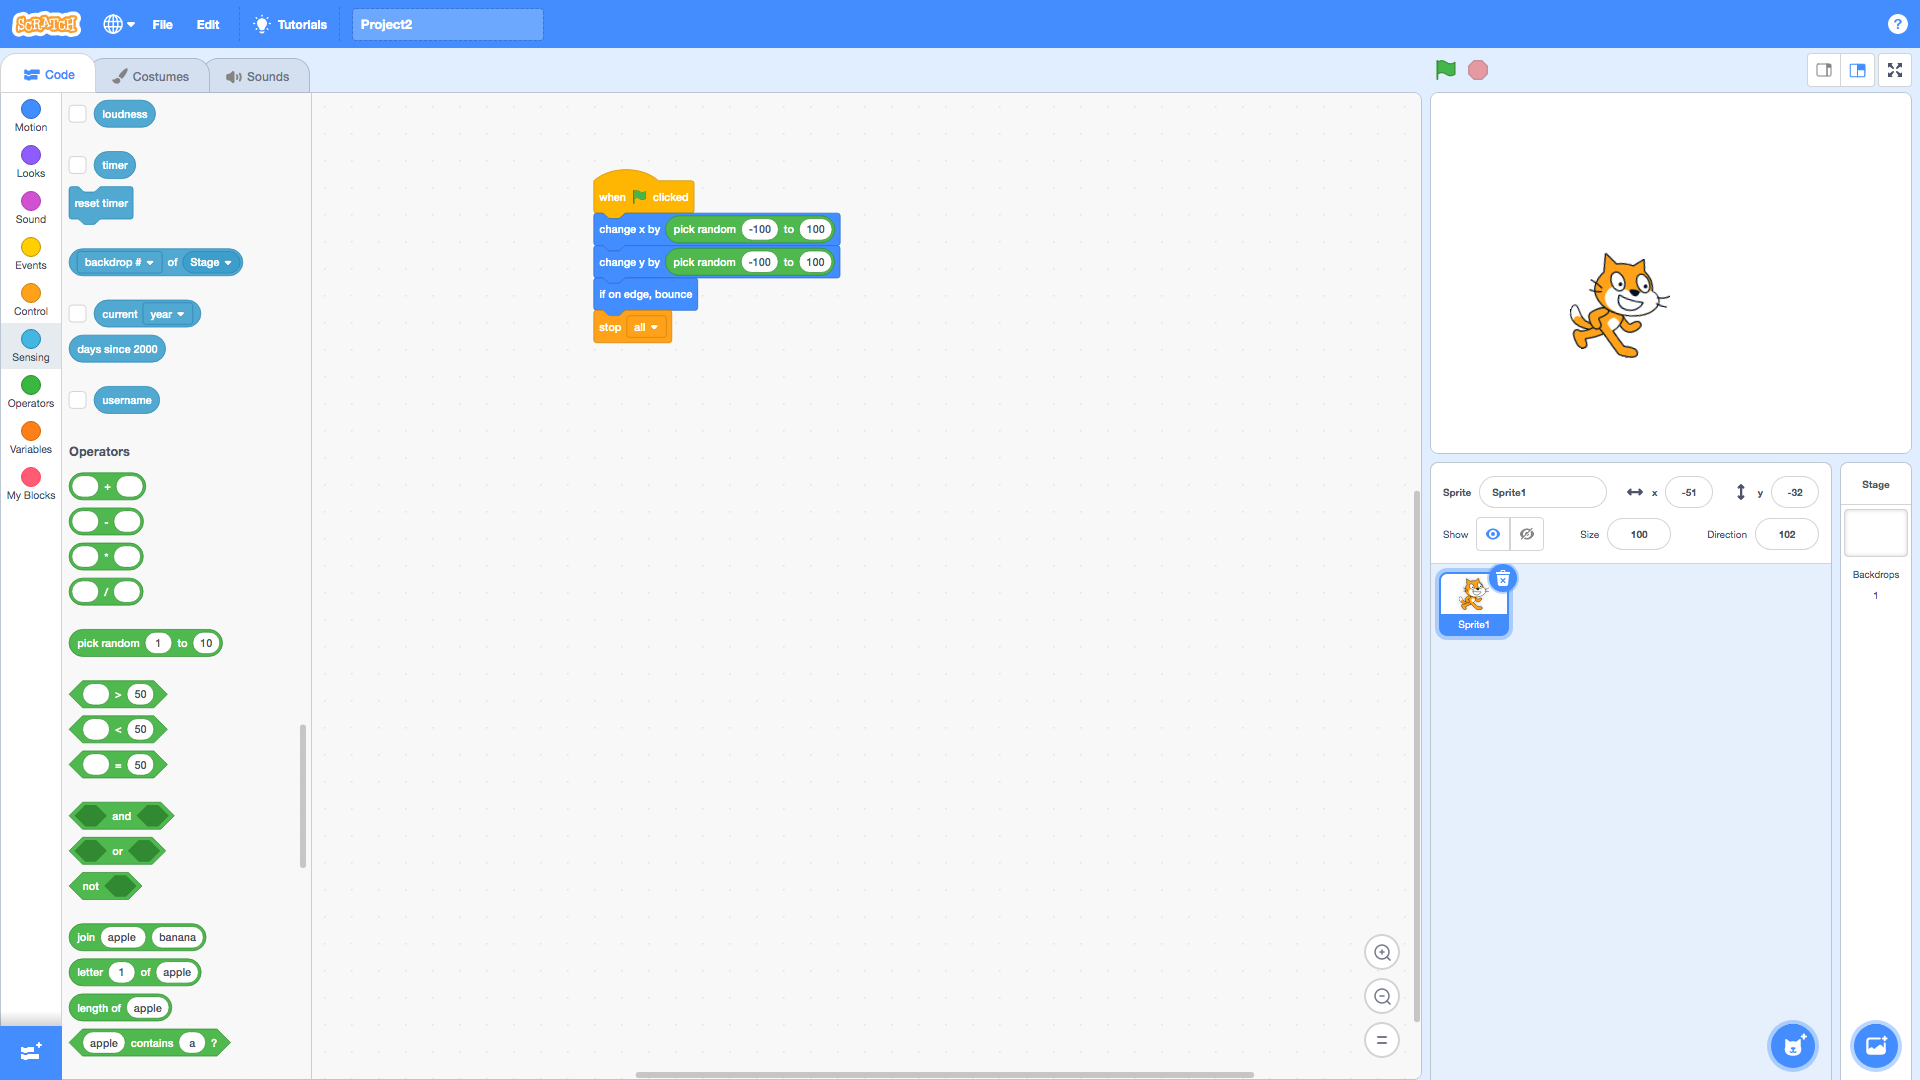
\includegraphics[width=1.0\linewidth,height=0.5\linewidth]{fig0066.png}
  \caption{Отскачане от ръбовете}
\label{fig0066}
\end{figure}

Следващо, много полезно блокче, от групата на тъмно оранжевите е блокчето за изчакване на период от време (Фиг. \ref{fig0067}). Когато това блокче бъде поставено между блокчетата за начало и край, програмата изчаква зададения брой секунди, преди да преустанови изпълнението си. По време на изпълнение, ясно може да се забележи, че около последователността от инструкции се появява жълта рамка, която символизира режима на изпълняващи се инструкции. 

\begin{figure}[H]
  \centering
  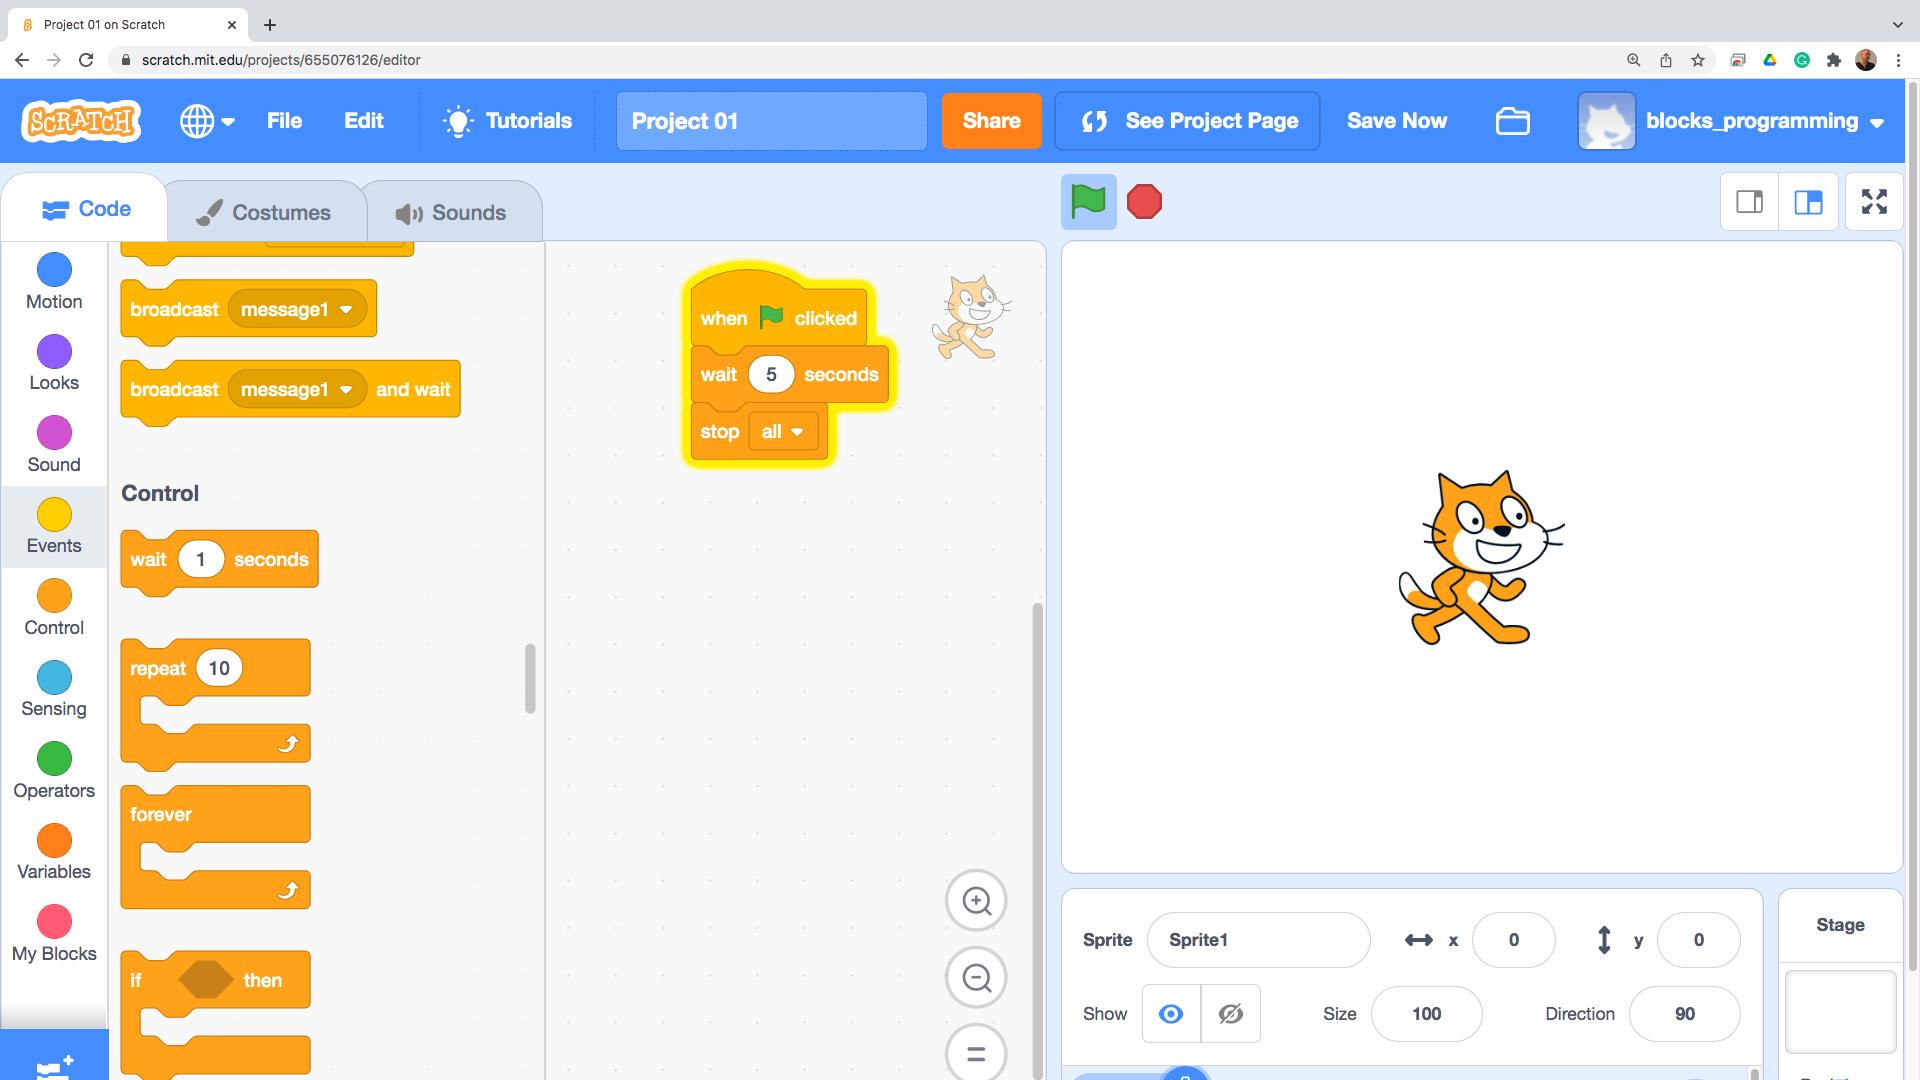
\includegraphics[width=1.0\linewidth,height=0.5\linewidth]{fig0067.png}
  \caption{Инструкция за изчакване}
\label{fig0067}
\end{figure}

Групата на лилавите блокчета съдържат инструкции за външното оформление на анимирания герой. Първите две блокчета са предназначени за реплики (Фиг. \ref{fig0068}), които героят казва (изписват се както в комикс). Първото блокче задава текст, който стои на екрана до следващата инструкция. Точно за това е нужно да има няколко секунди изчакване, така че текстът да остане видим за потребителя. Второто блокче има и параметър с който да се определи колко секунди текстът да бъде видим за потребителя. 

\begin{figure}[H]
  \centering
  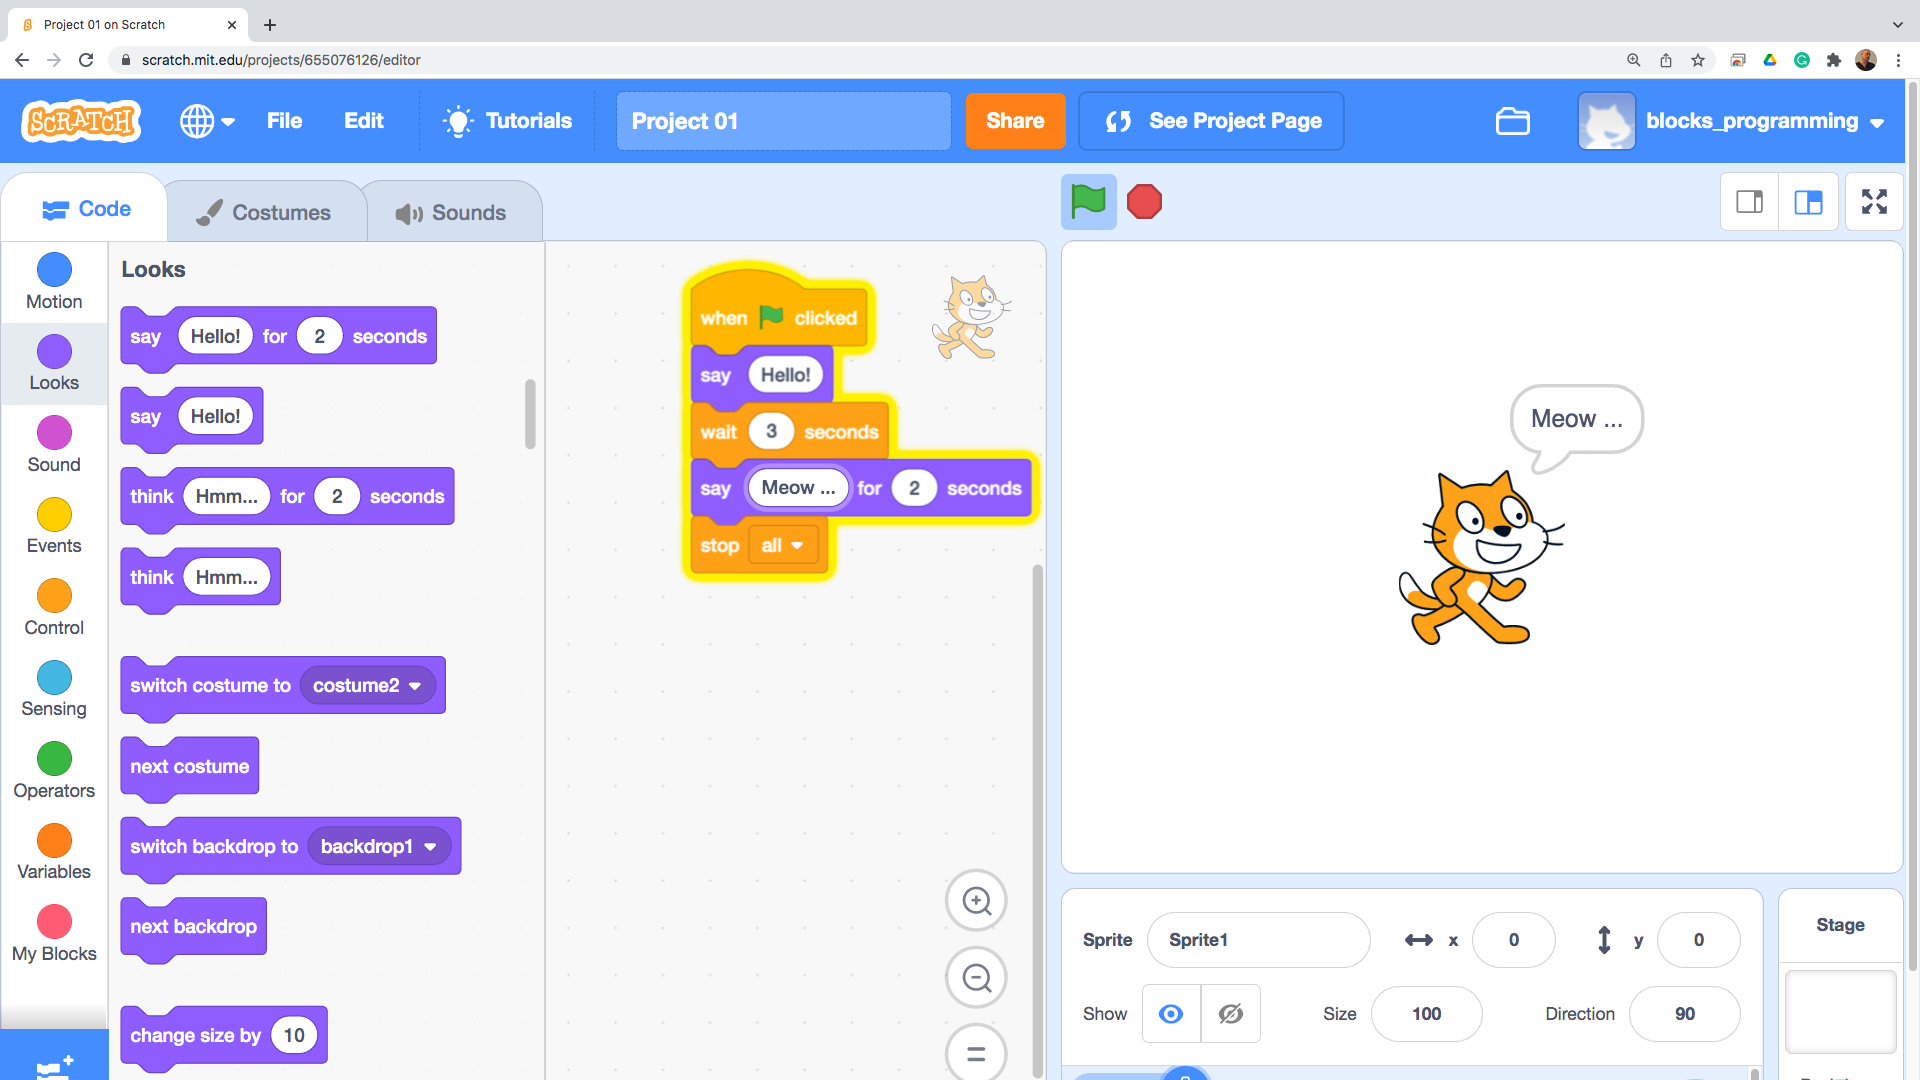
\includegraphics[width=1.0\linewidth,height=0.5\linewidth]{fig0068.png}
  \caption{Изписване на реплики за изговаряне}
\label{fig0068}
\end{figure}

Вторите две блокчета са предвидени за реплики, които анимираният герой си мисли, но не изрича. Разликата се състои в начина по който се визуализира текстът (Фиг. \ref{fig0069}).

\begin{figure}[H]
  \centering
  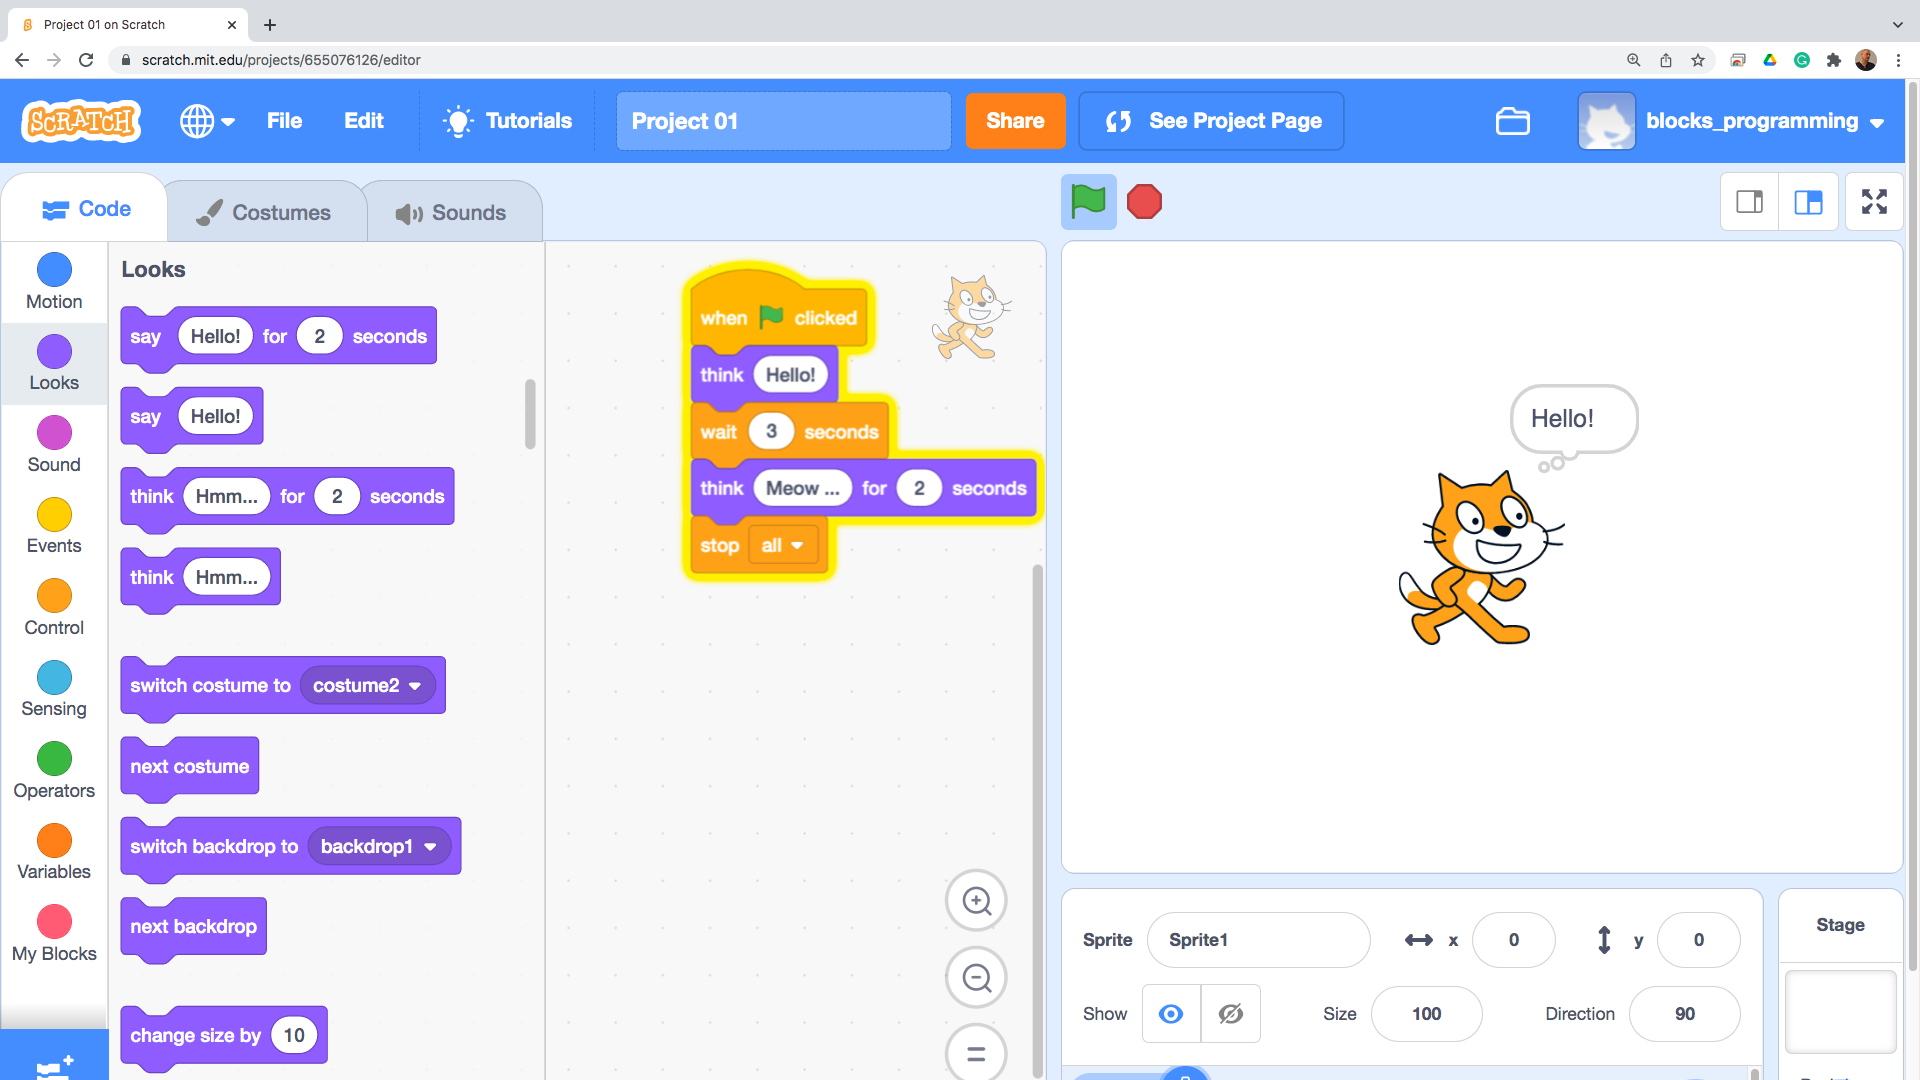
\includegraphics[width=1.0\linewidth,height=0.5\linewidth]{fig0069.png}
  \caption{Изписване на реплики, като мисъл}
\label{fig0069}
\end{figure}

Анимираните герои в Scratch са под формата на спрайтове. Спрайтът е набор от различни изображения за героя в различни пози. За смяната на тези различни пози се използват две блокчета (Фиг. \ref{fig0070}), като първото задава конкретен кадър в спрайта, а второто задава следващия кадър в последователността.

\begin{figure}[H]
  \centering
  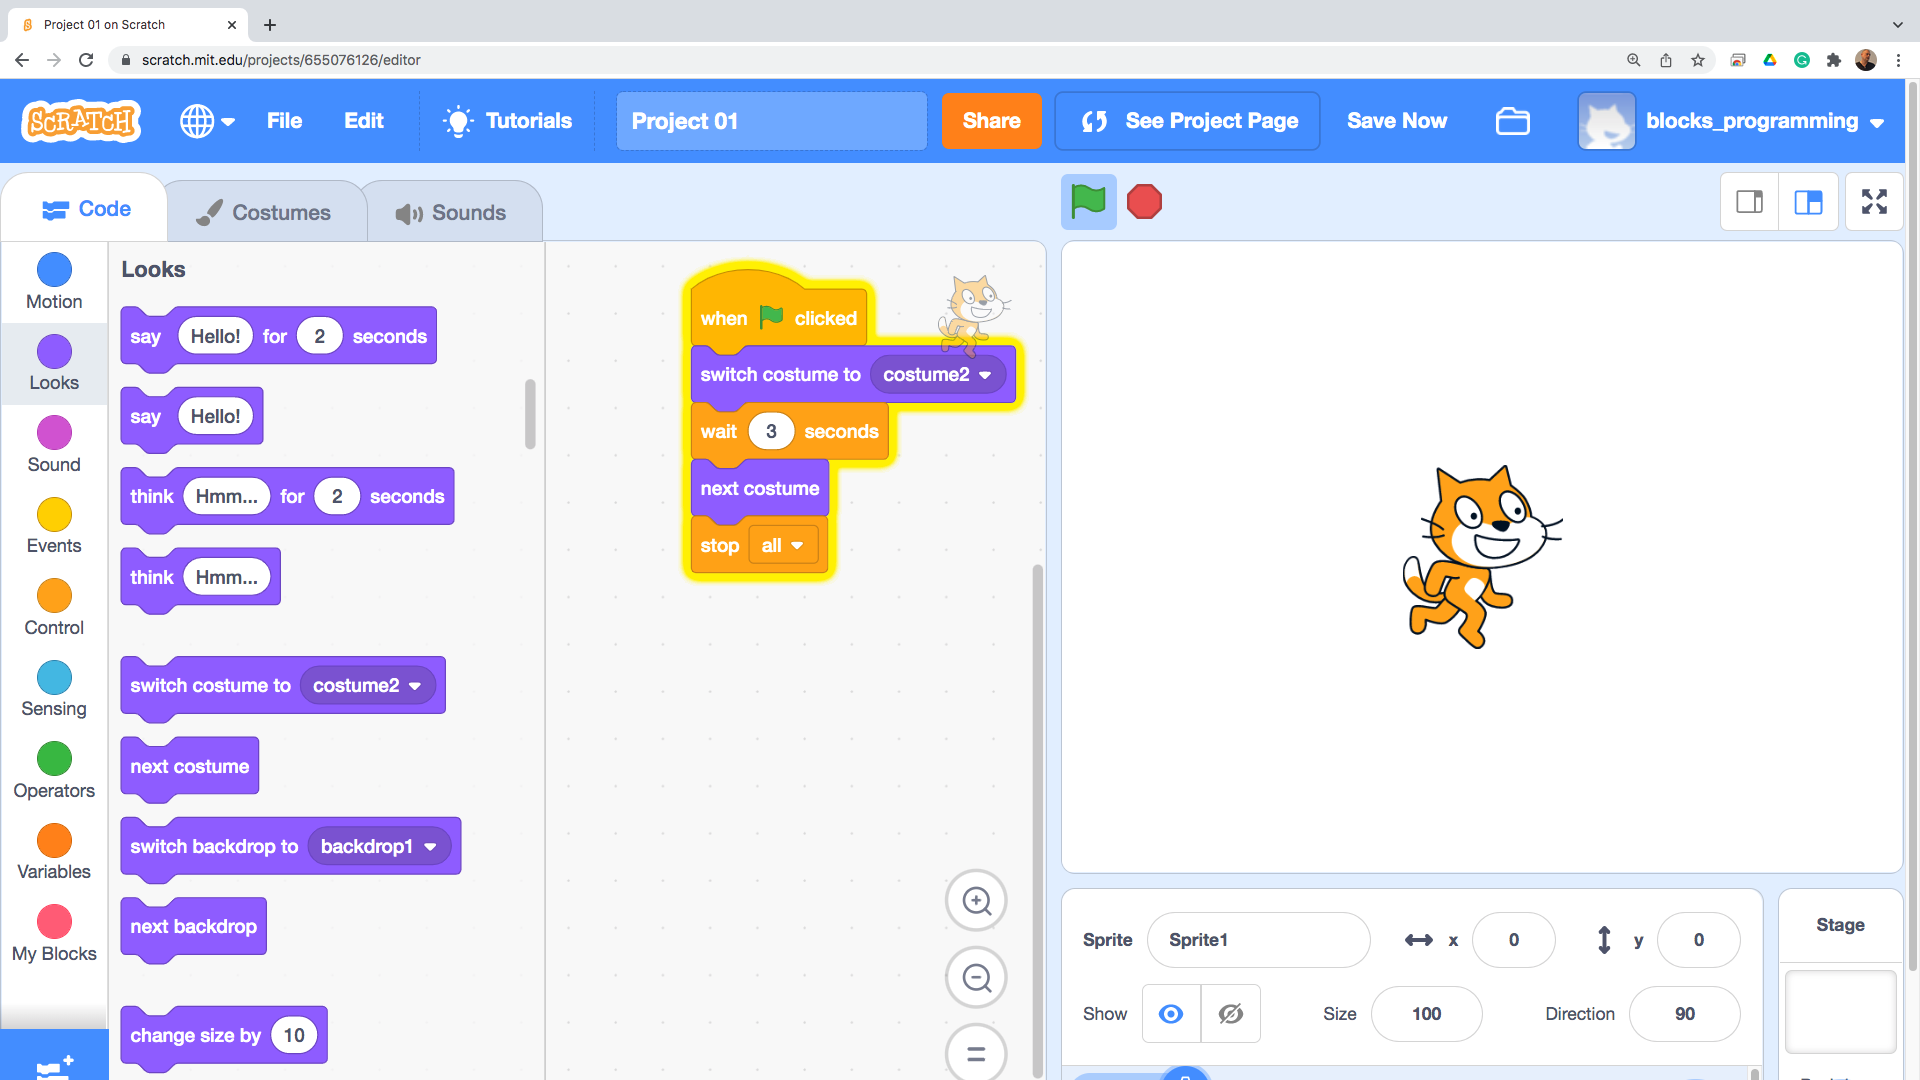
\includegraphics[width=1.0\linewidth,height=0.5\linewidth]{fig0070.png}
  \caption{Смяна на пози}
\label{fig0070}
\end{figure}

На работната сцена освен анимираните герои (под формата на спрайтове) има и фоново изображение. Това фоново изображение също подлежи на промяна, за което са предвидени две отделни блочета (Фиг. \ref{fig0071}). С първото може да се избират фонови изображения напред, назад, по случаен принцип или с конкретно название, а с второто блокче следващото изображение в последователността. 

\begin{figure}[H]
  \centering
  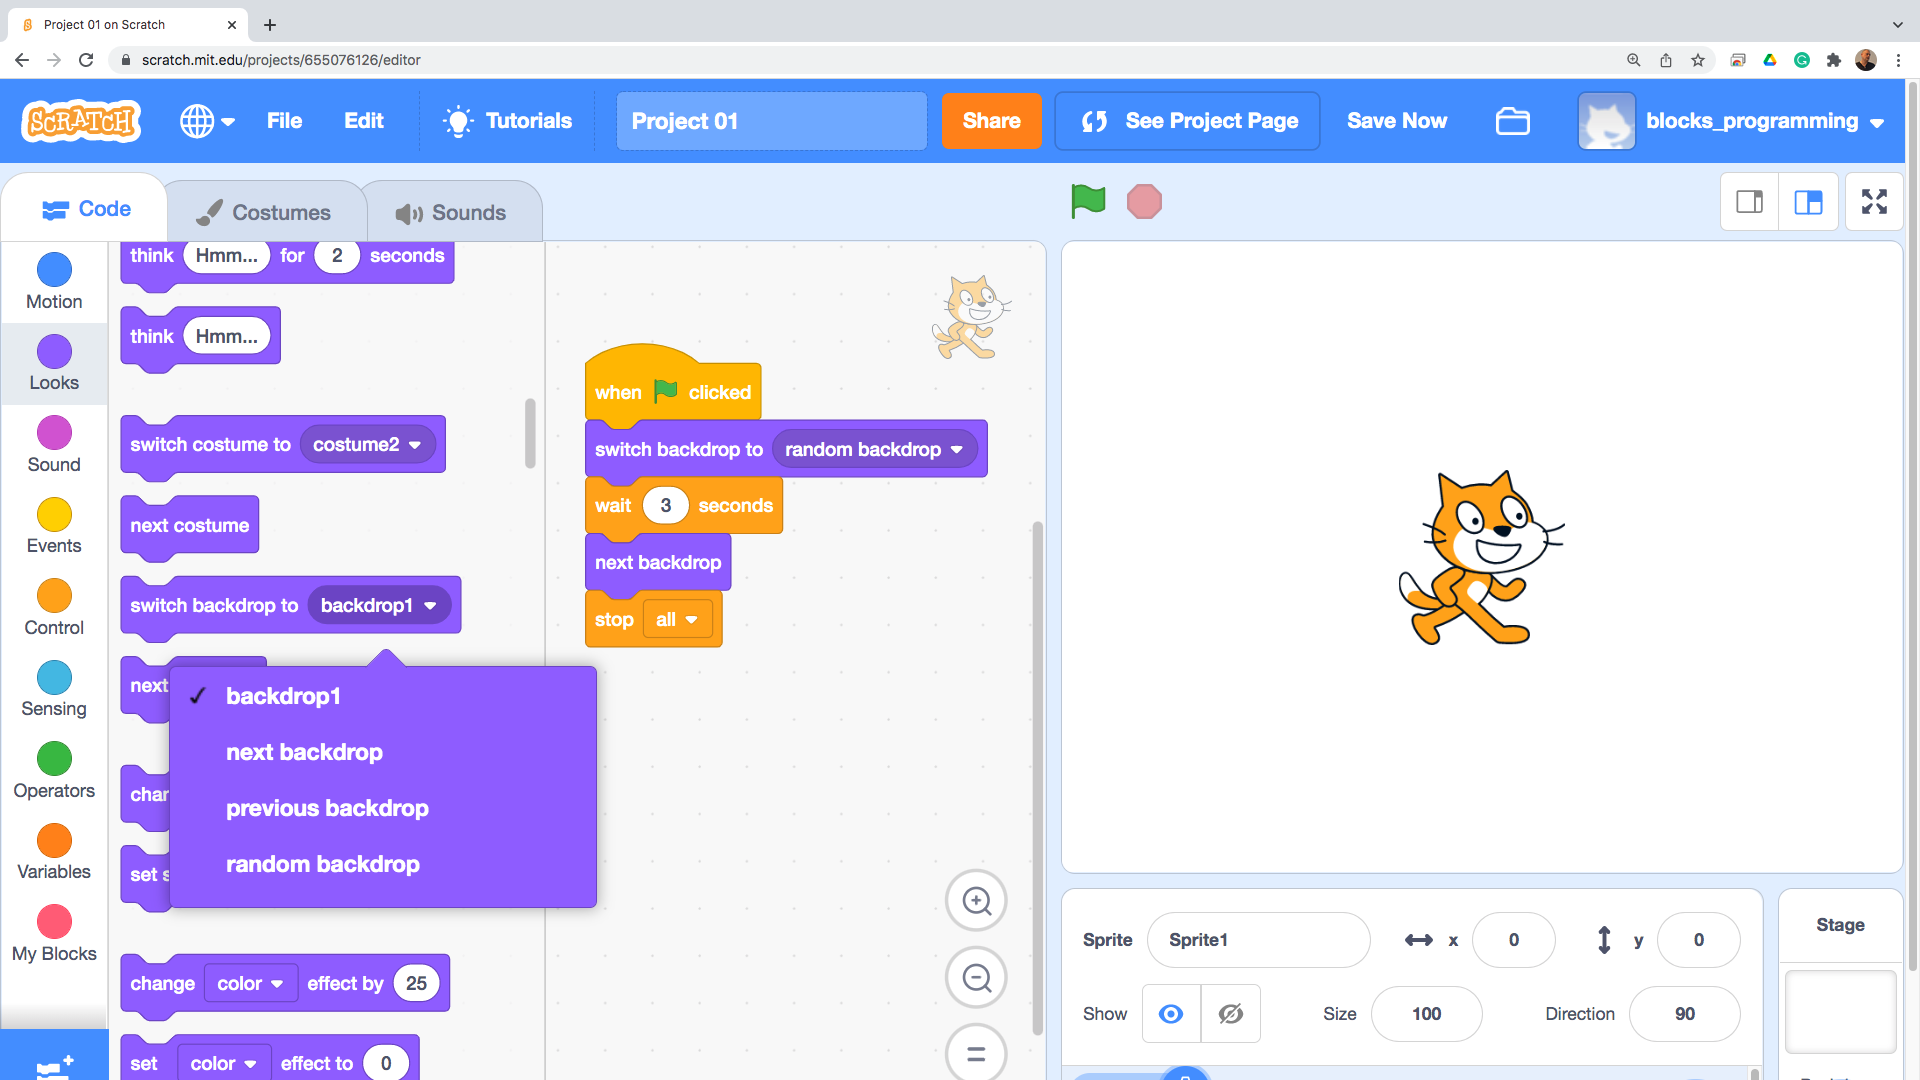
\includegraphics[width=1.0\linewidth,height=0.5\linewidth]{fig0071.png}
  \caption{Смяна на фона}
\label{fig0071}
\end{figure}

За промяната на размера на анимирания герой има две конкретни блокчета, като първото променя размера в абсолютни стойности, а второто променя размера в проценти, спрямо оригиналния размер (Фиг. \ref{fig0072}).

\begin{figure}[H]
  \centering
  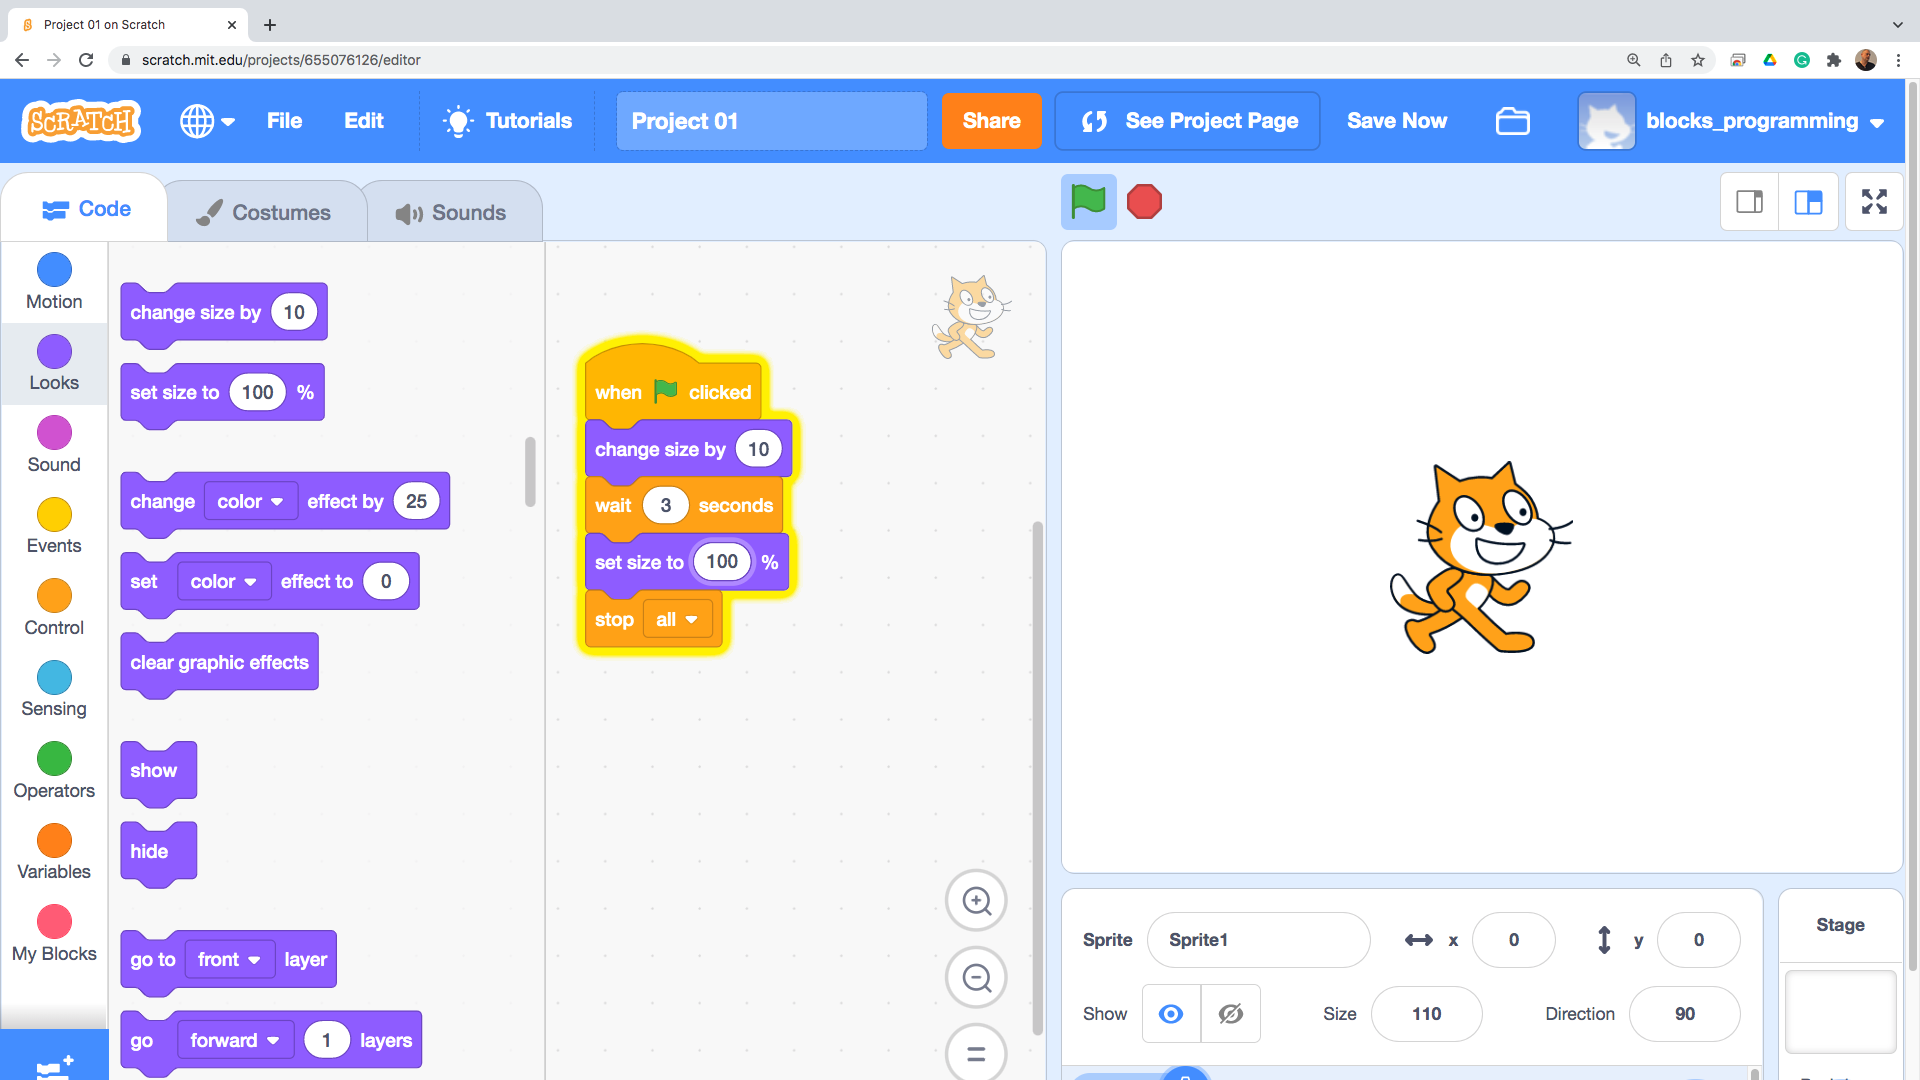
\includegraphics[width=1.0\linewidth,height=0.5\linewidth]{fig0072.png}
  \caption{Промяна на размерите}
\label{fig0072}
\end{figure}

За промяна на визуалното оформление на анимирания герой са предвидени три блокчета (Фиг. \ref{fig0073}). Първите две задават промяна, като промяната може да бъде в цвета, различни изкривявания, пикселизация, мозайка, прозрачност или яркост, а третото блокче отменя всички направени декорации. Първото блокче предизвиква относителна промяна, спрямо текущото състояние на героя, а второто блокче задава абсолютна промяна. Отново е важно да се дадат няколко секунди, така че промените да бъдат ясно различими. 

\begin{figure}[H]
  \centering
  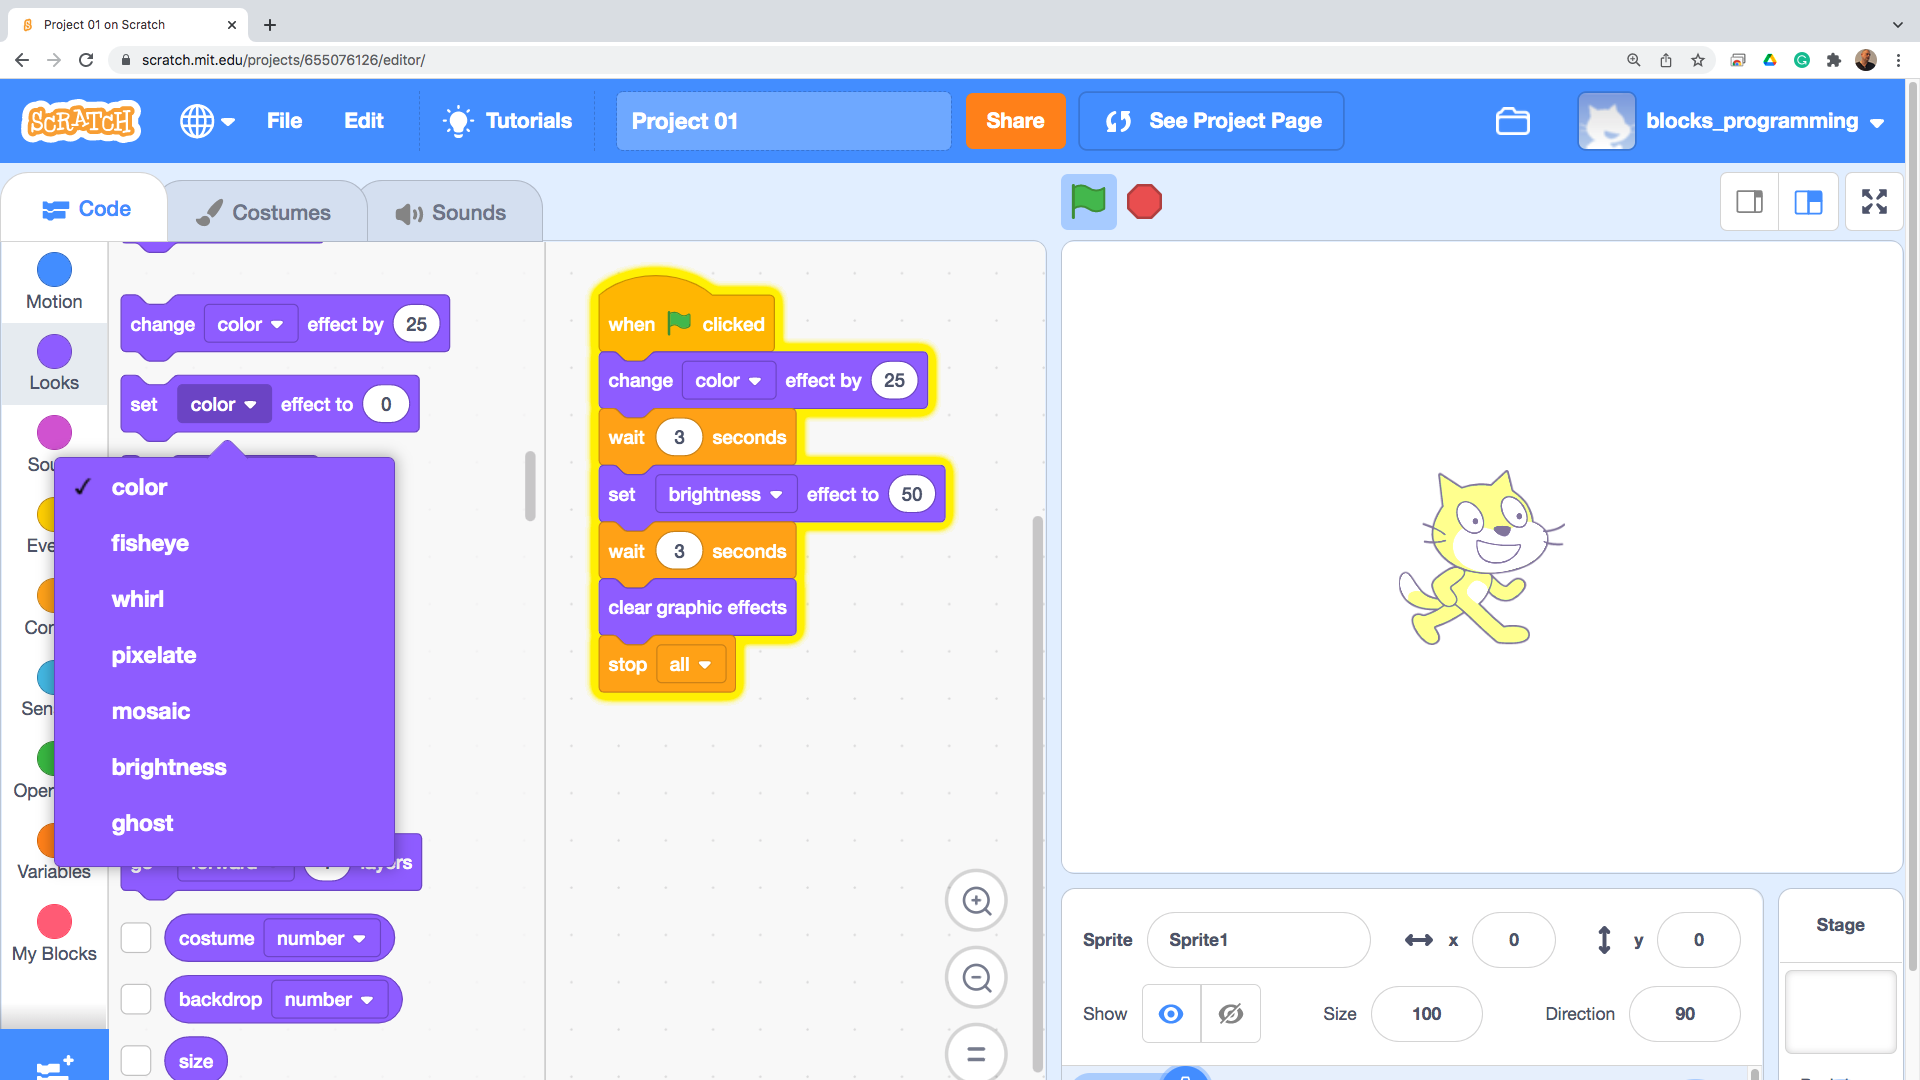
\includegraphics[width=1.0\linewidth,height=0.5\linewidth]{fig0073.png}
  \caption{Промяна на външния вид}
\label{fig0073}
\end{figure}

Работата със спрайтове е предимно за постигане на анимирани ефекти. Различните анимирани герой в сцената имат определени взаимодействия по между си. Сценарият на изработвания проект определя в кой момент всеки от героите се появява на сцената и в кой момент изчезва. За да се осъществи появата и изчезването са предвидени две блокчета, извършващи тези действия (Фиг. \ref{fig0074}).

\begin{figure}[H]
  \centering
  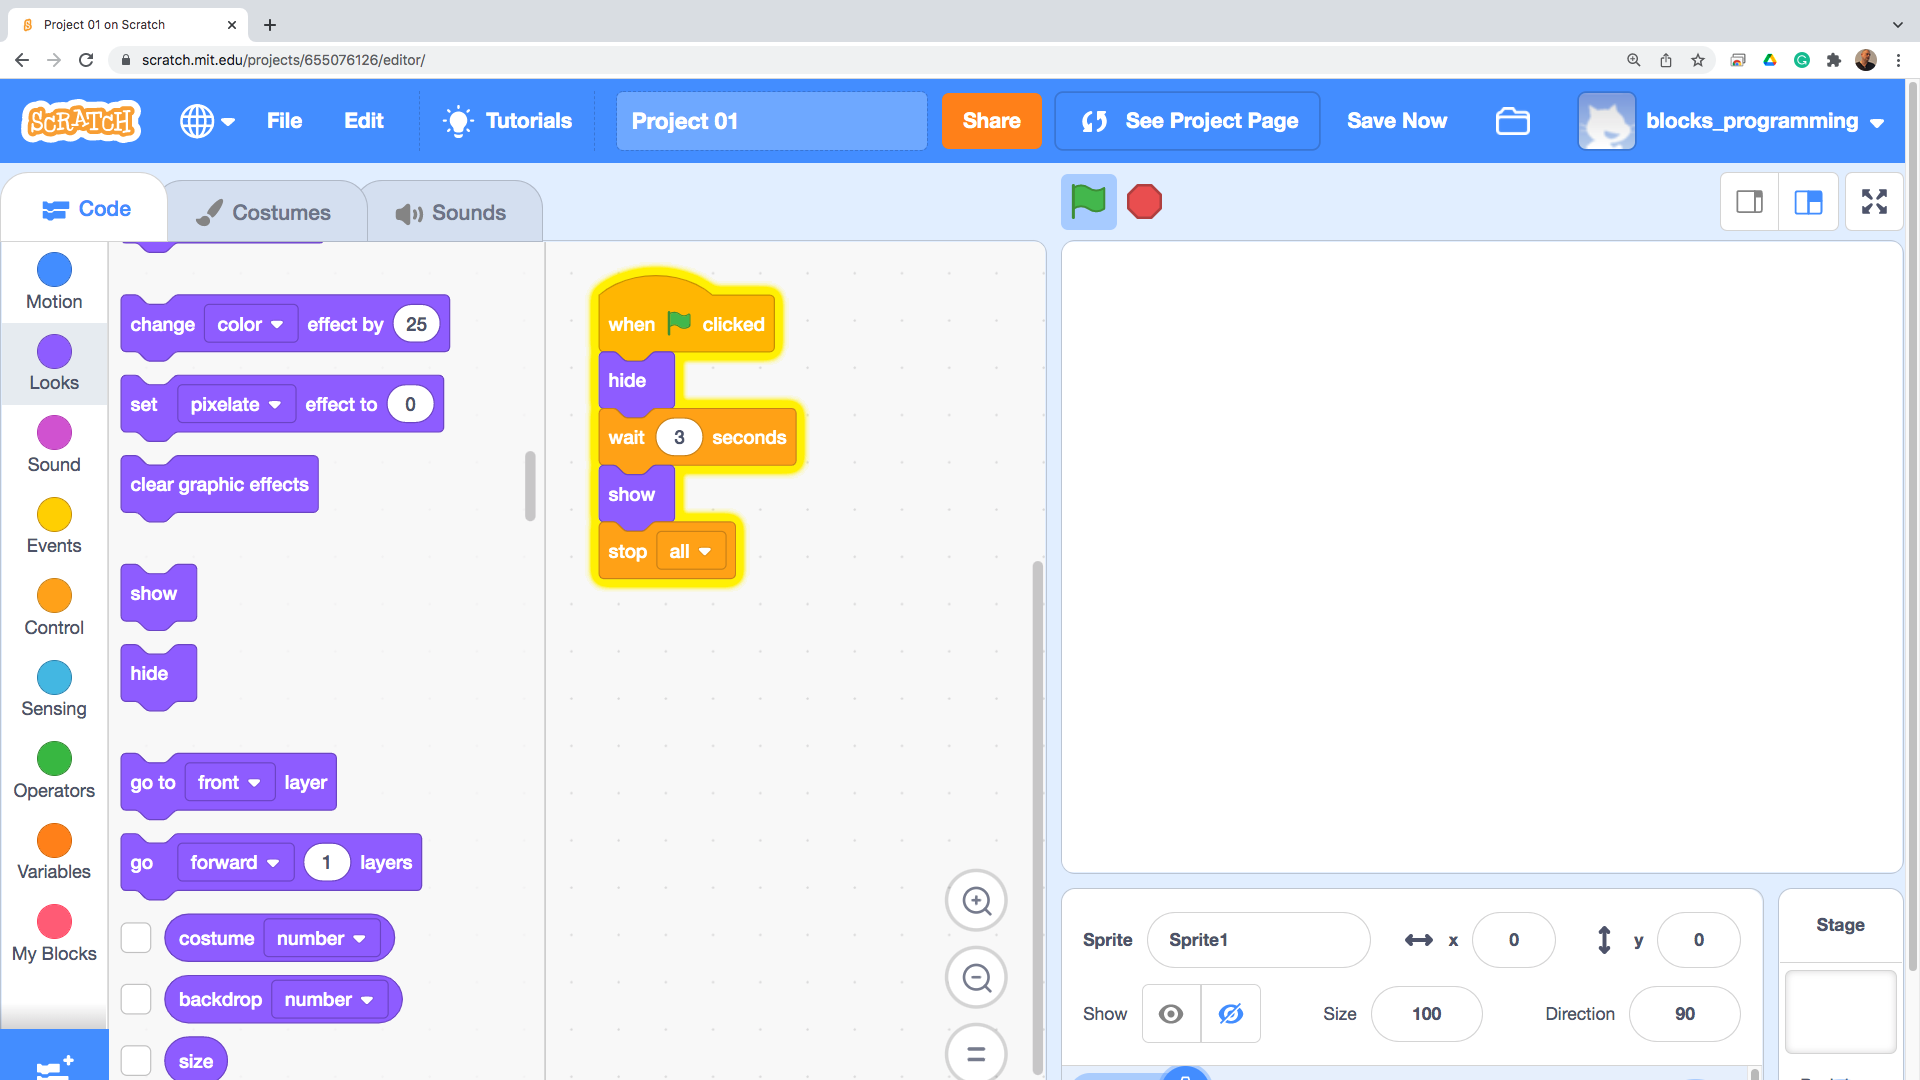
\includegraphics[width=1.0\linewidth,height=0.5\linewidth]{fig0074.png}
  \caption{Скриване и повява}
\label{fig0074}
\end{figure}

Множество програмни продукти, работещи с растерни графични изображения, организират различните изображения в слоеве. Пример за такива са Adobe Photoshop, GIMP, Microsoft Word, LibreOffice Draw и много други. Организацията в слоеве е логична, тъй като различните спрайтове в определени моменти от времето могат да се припокриват. В някои от софтуерните пакети за графична обработка, наличието на слоеве се възприема като Z буфер. В Scratch също е налична възможността за работа със слоеве, като две конкретни блокчета позволяват спрайтът да се придвижва напред и назад по слоевете (Фиг. \ref{fig0075}).

\begin{figure}[H]
  \centering
  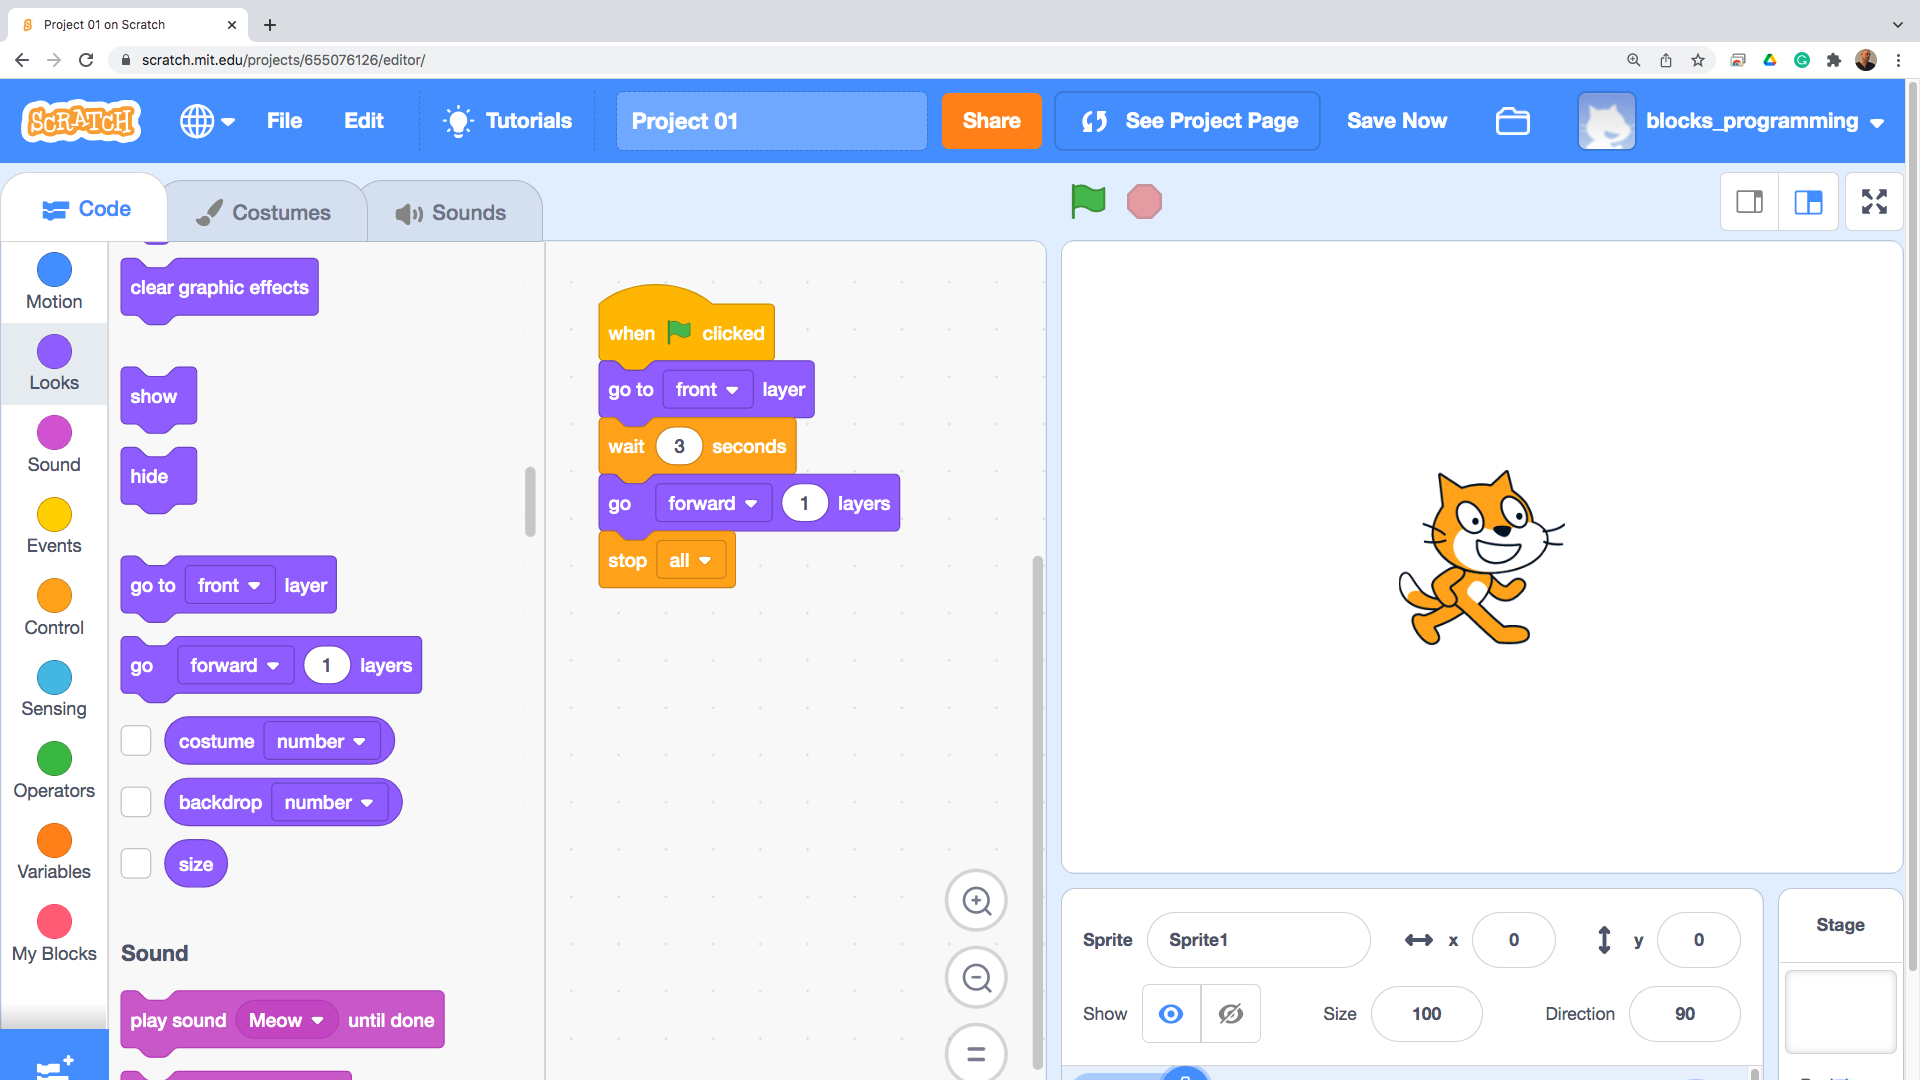
\includegraphics[width=1.0\linewidth,height=0.5\linewidth]{fig0075.png}
  \caption{Придвижване по слоевете}
\label{fig0075}
\end{figure}

Групата блокчета в пурпурен цвят са предназначени за звуково оформление. Изпълнението на звуци се постига с първите две блокчета в групата (Фиг. \ref{fig0076}). Първото блокче изпълнява звука докато той бъде приключен, а второто блокче го стартира и предава изпълнението към следващото блокче. С третото блокче всички изпълняващи се звуци биват спрени. Програмната среда позволява звуци да бъдат записани и от компютъра на потребителя. 

\begin{figure}[H]
  \centering
  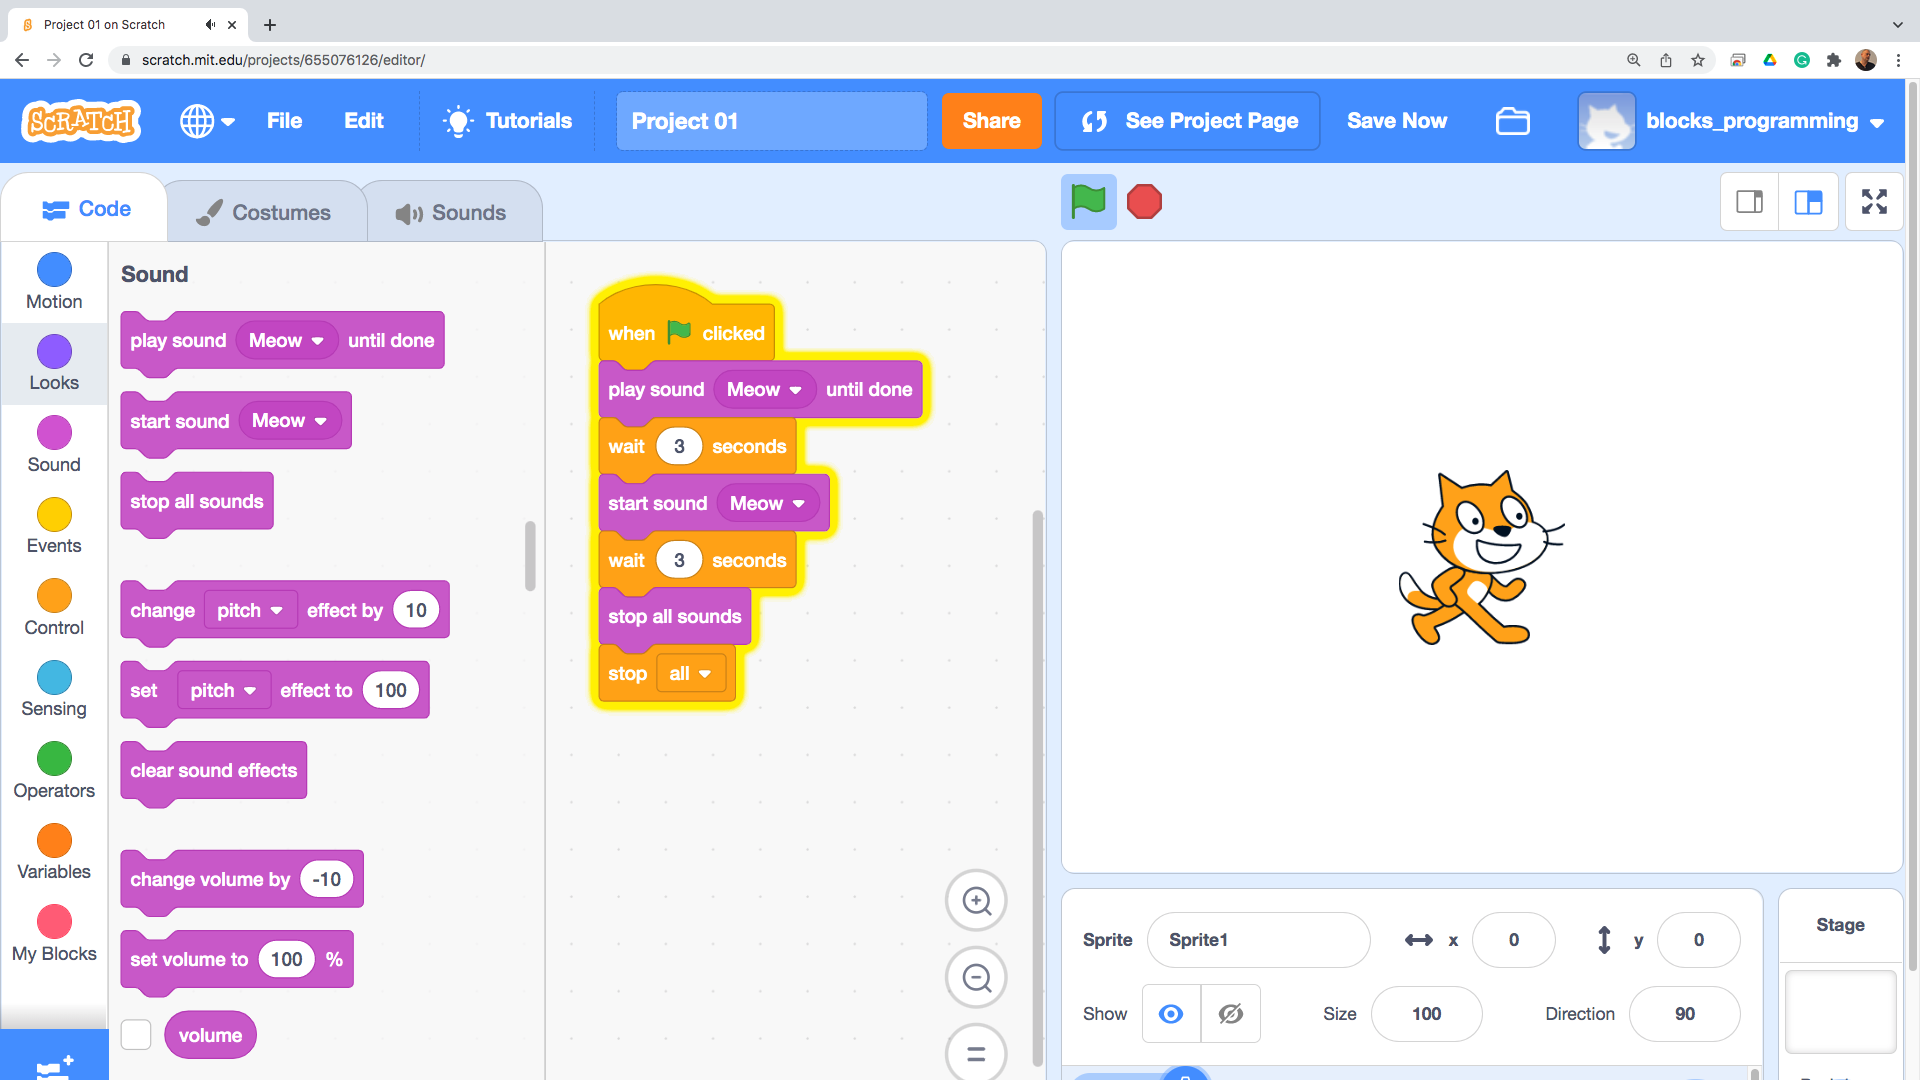
\includegraphics[width=1.0\linewidth,height=0.5\linewidth]{fig0076.png}
  \caption{Изпълнение на звуци}
\label{fig0076}
\end{figure}

Две от характеристиките на звуците могат да се променят с блокчетата за височина (честотна) и стерео озвучаване (ляво/дясно). И двете блокчета имат числени стойности за посочените характеристики (Фиг. \ref{fig0077}).

\begin{figure}[H]
  \centering
  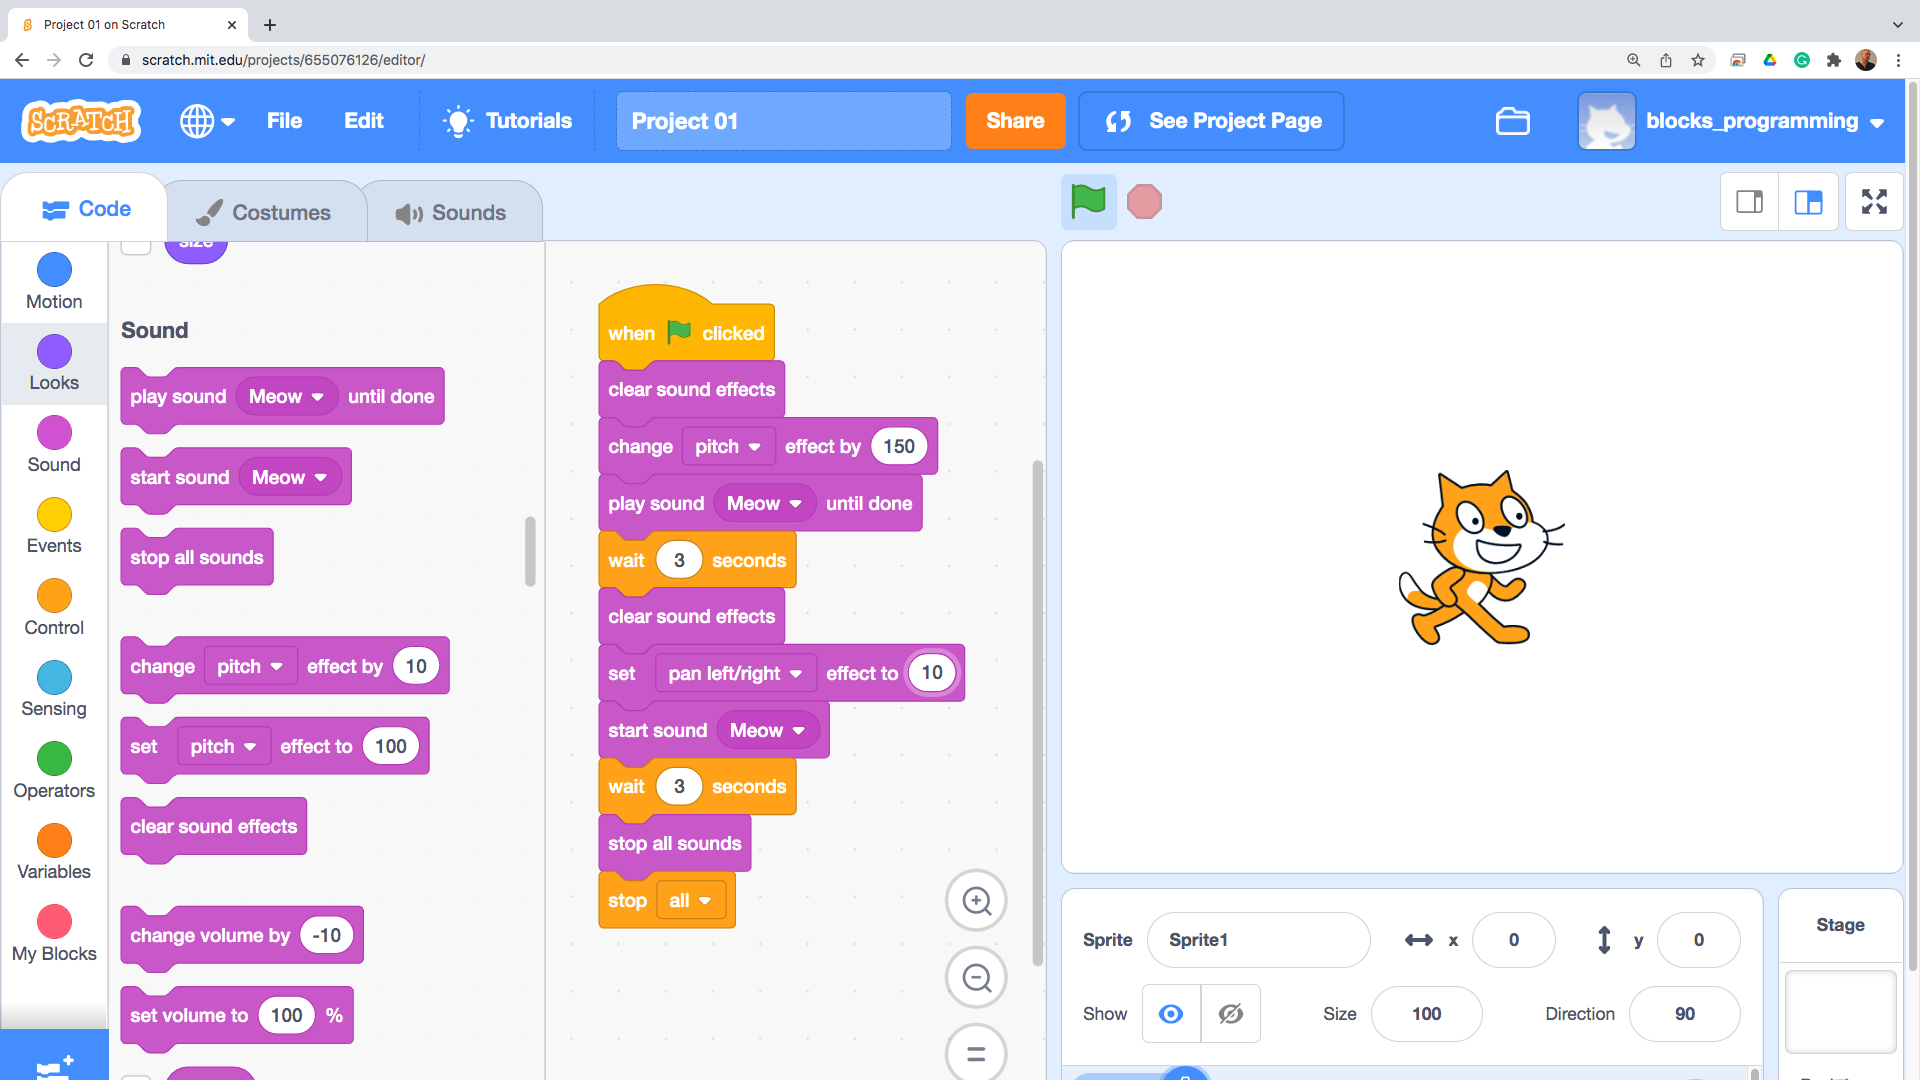
\includegraphics[width=1.0\linewidth,height=0.5\linewidth]{fig0077.png}
  \caption{Характеристики на звука}
\label{fig0077}
\end{figure}

За постигането на една по-богата звукова картина, силата на различните звуци може да се управлява с две блокчета (Фиг. \ref{fig0078}). Първото контролира силата на звука по абсолютна стойност, а второто като проценти. 

\begin{figure}[H]
  \centering
  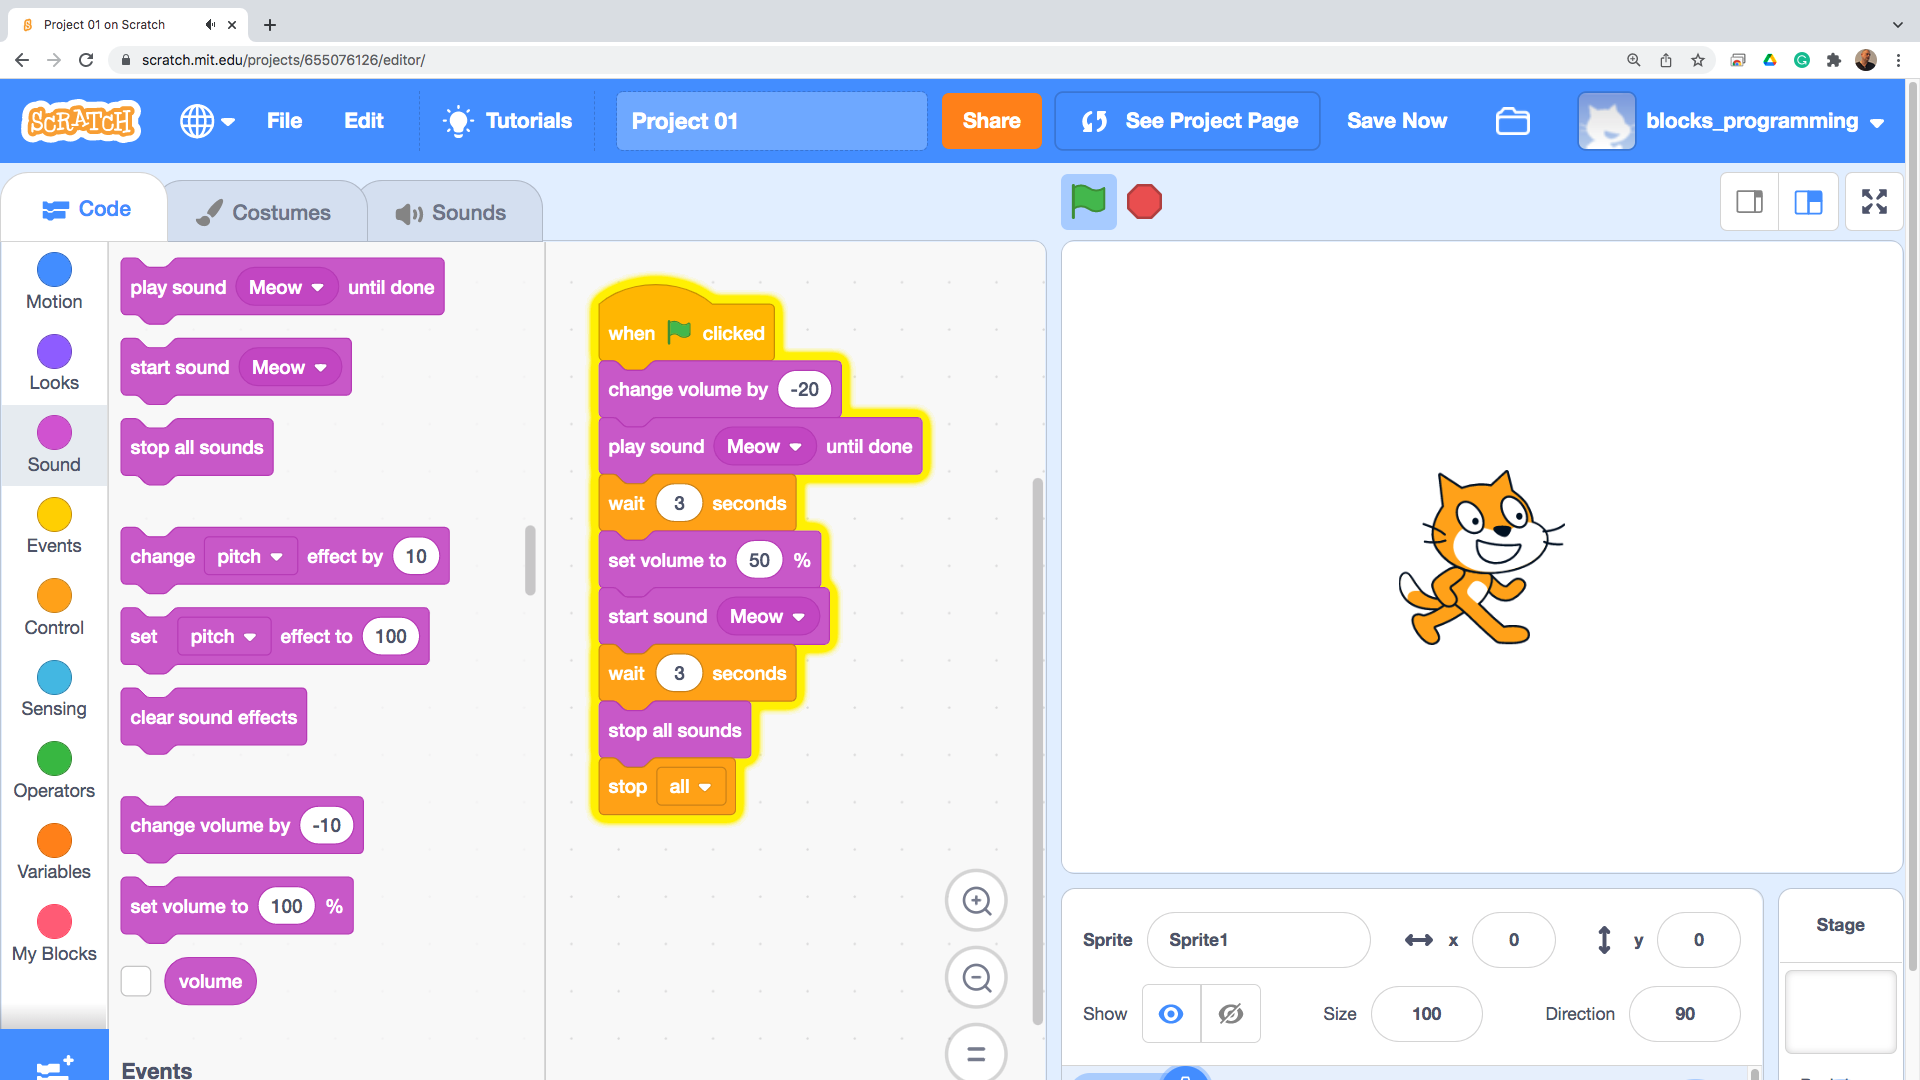
\includegraphics[width=1.0\linewidth,height=0.5\linewidth]{fig0078.png}
  \caption{Сила на звука}
\label{fig0078}
\end{figure}

Оранжевата група блокчета са предназначени за възникване на събития. Събитията са инструмент за изпълнение на инструкции, когато няма ясна престава за момента в който програмните инструкции трябва да се изпълнят. Такова събитие е натискане на бутон по клавиатурата от страна на потребителя (Фиг. \ref{fig0079}).

\begin{figure}[H]
  \centering
  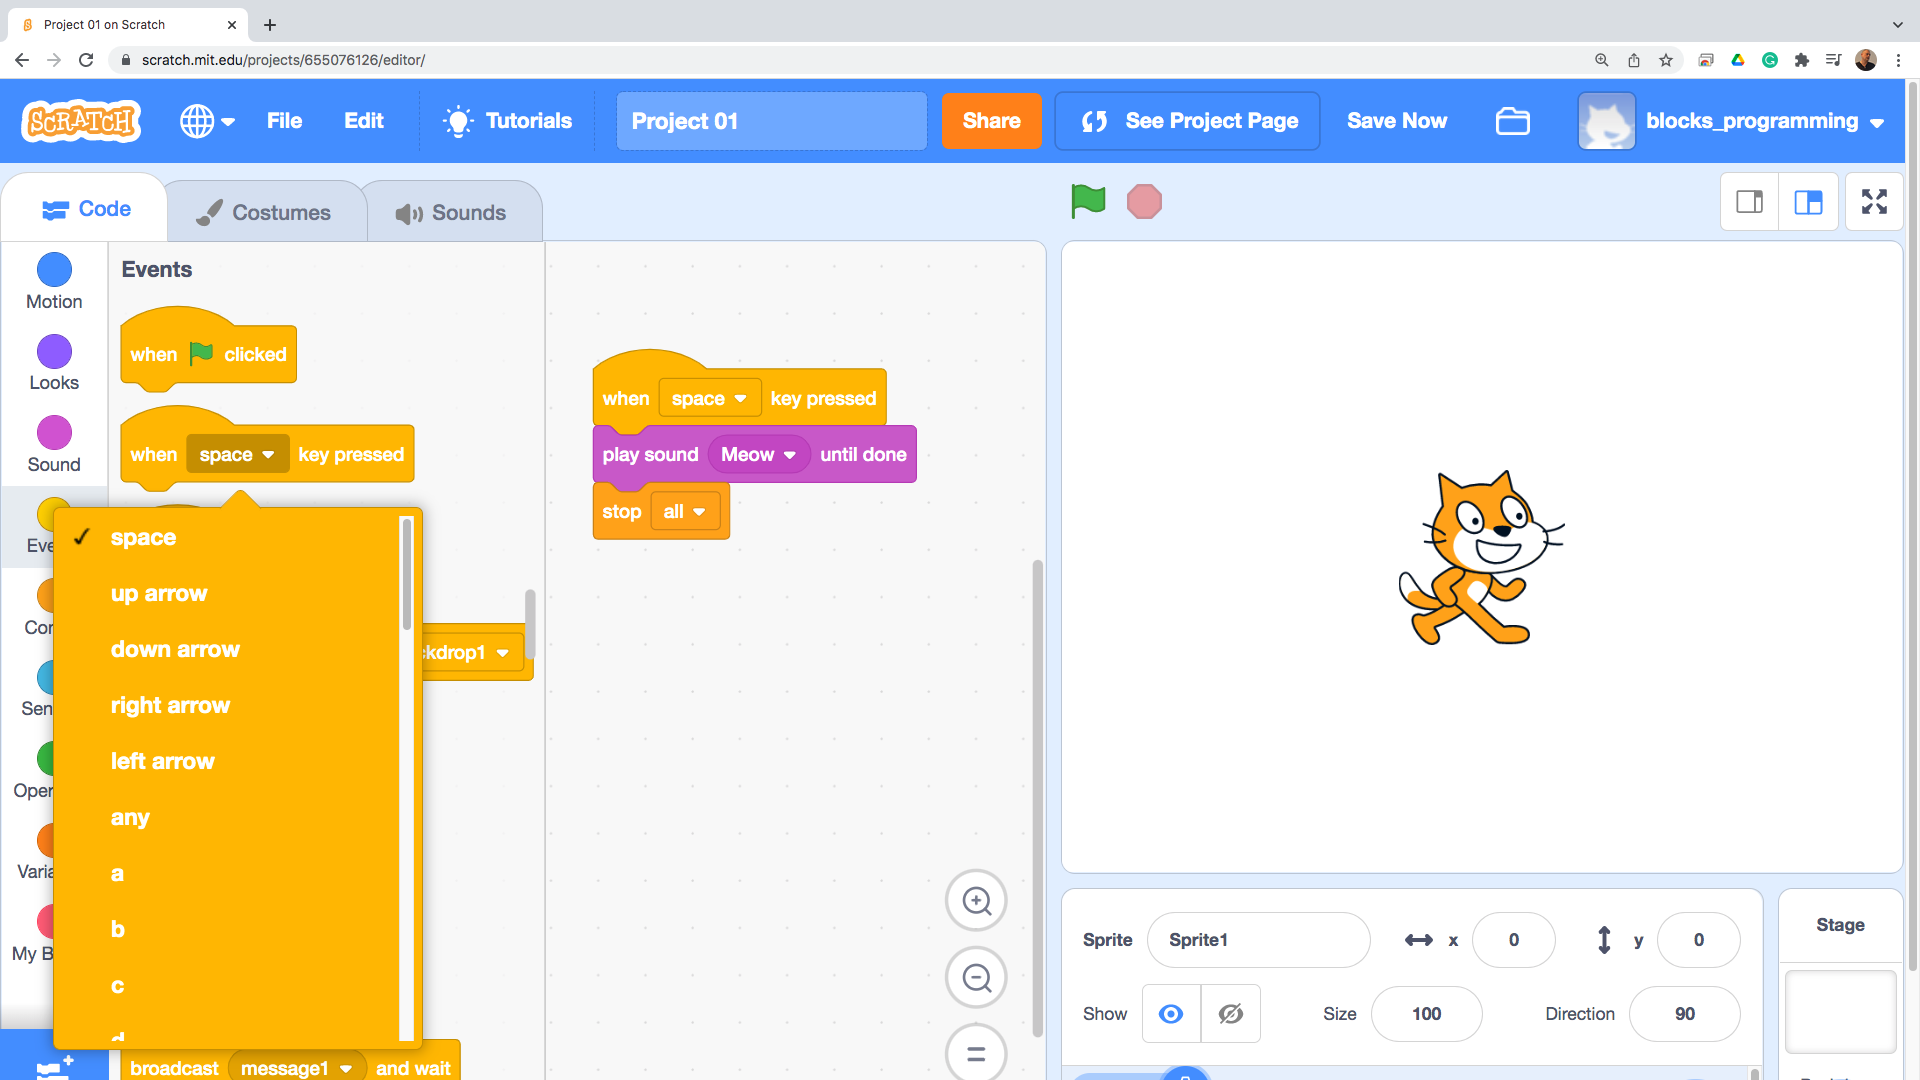
\includegraphics[width=1.0\linewidth,height=0.5\linewidth]{fig0079.png}
  \caption{Събитие за натискане на клавиш}
\label{fig0079}
\end{figure}

Кликването с мишката върху определен спрайт също може да бъде обработено с помощта на подходящо блокче (Фиг. \ref{fig0080}).

\begin{figure}[H]
  \centering
  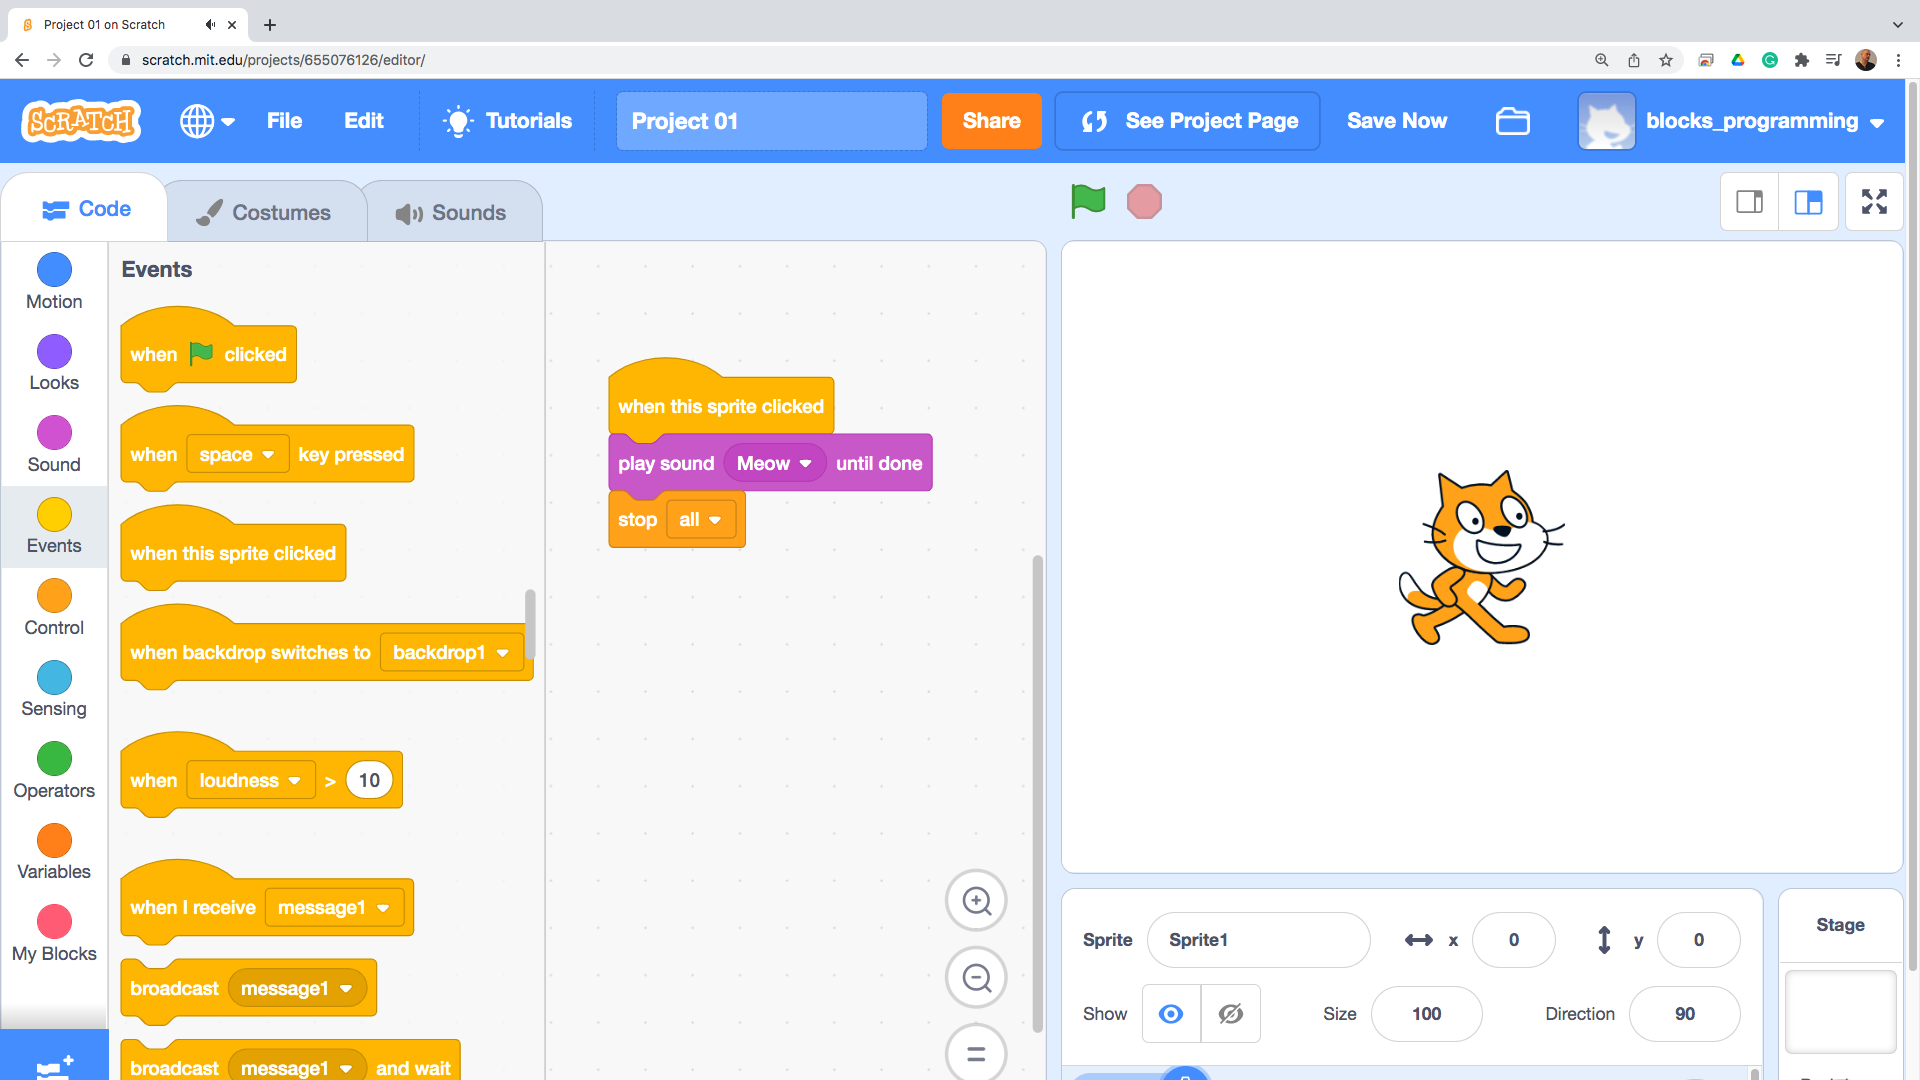
\includegraphics[width=1.0\linewidth,height=0.5\linewidth]{fig0080.png}
  \caption{Събитие за кликане с мишката}
\label{fig0080}
\end{figure}

Смяната на фона също може да предизвика обработване на събитие. За тази цел има предвидено блокче (Фиг. \ref{fig0081}).

\begin{figure}[H]
  \centering
  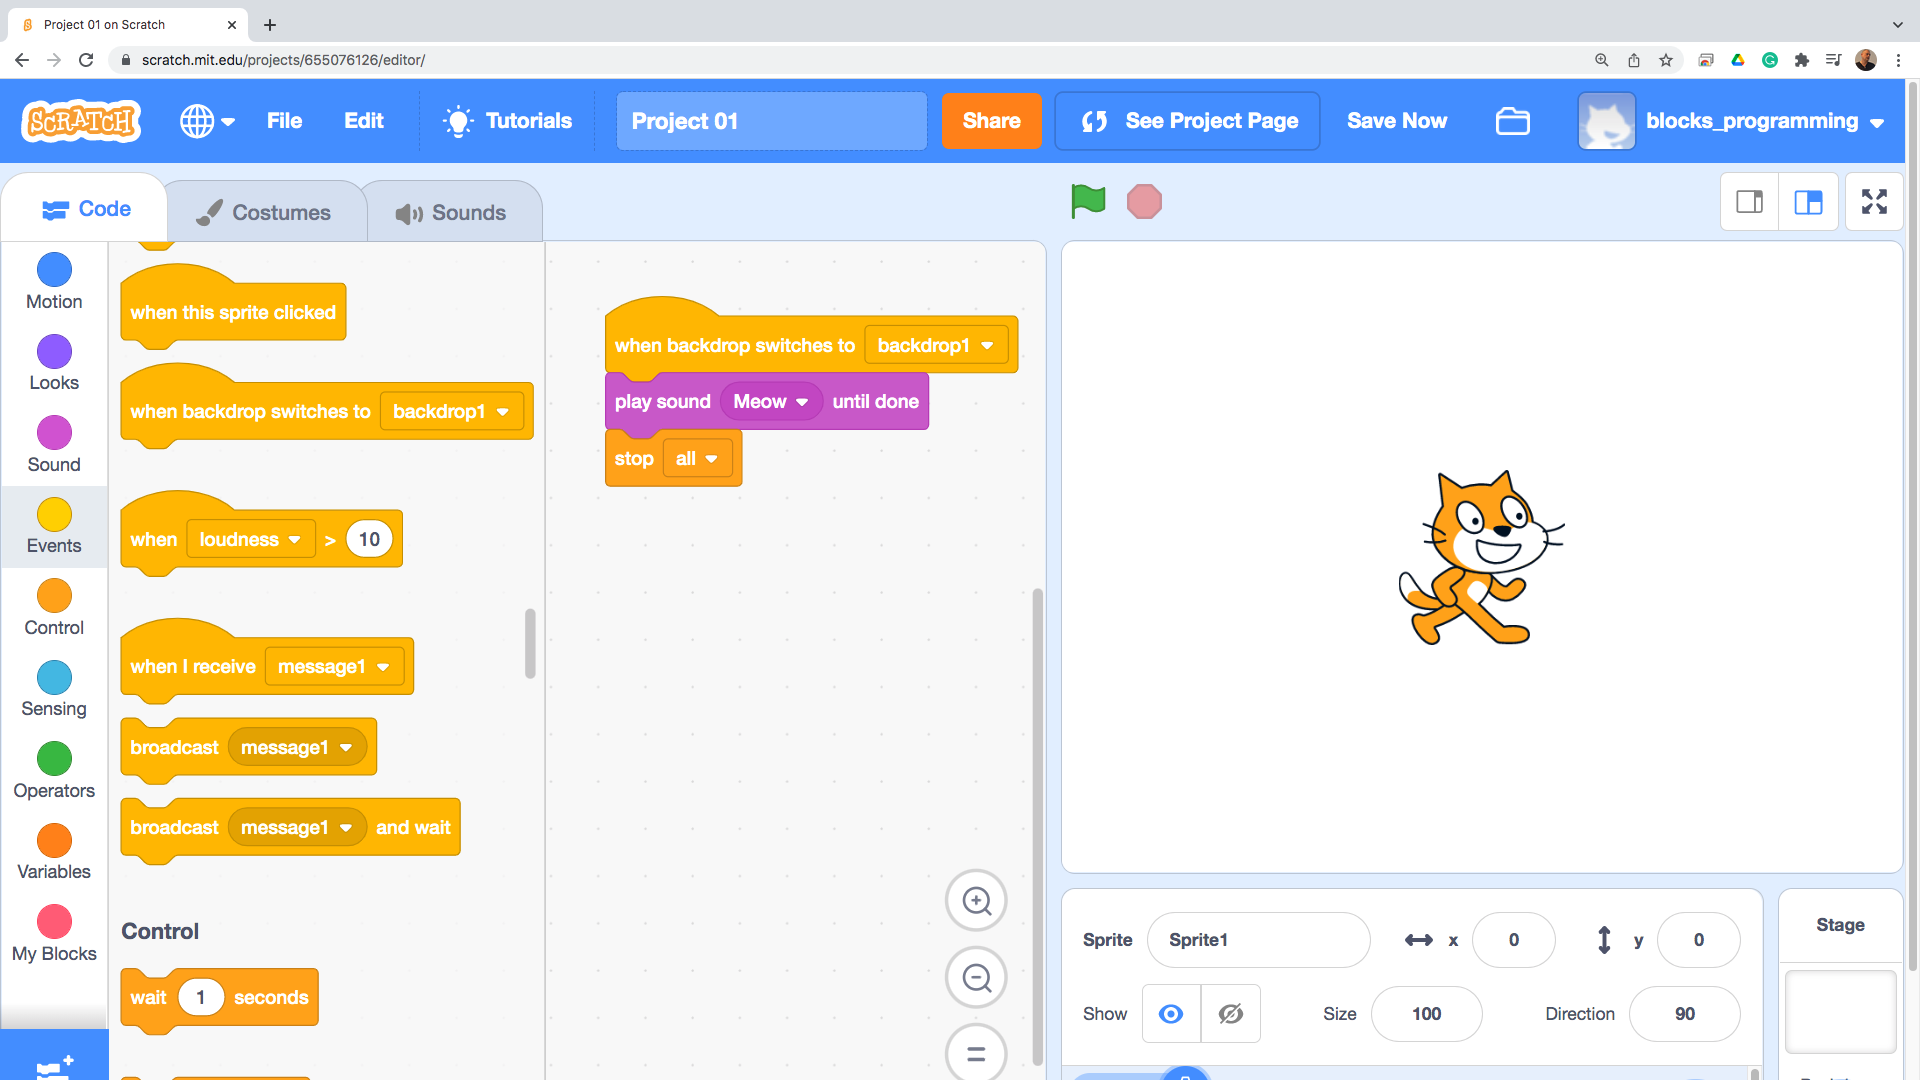
\includegraphics[width=1.0\linewidth,height=0.5\linewidth]{fig0081.png}
  \caption{Събитие за смяна на фона}
\label{fig0081}
\end{figure}

Събитие може да бъде прихванато след изтичане на определено време към таймер или достигане на определено ниво на звук (Фиг. \ref{fig0082}).

\begin{figure}[H]
  \centering
  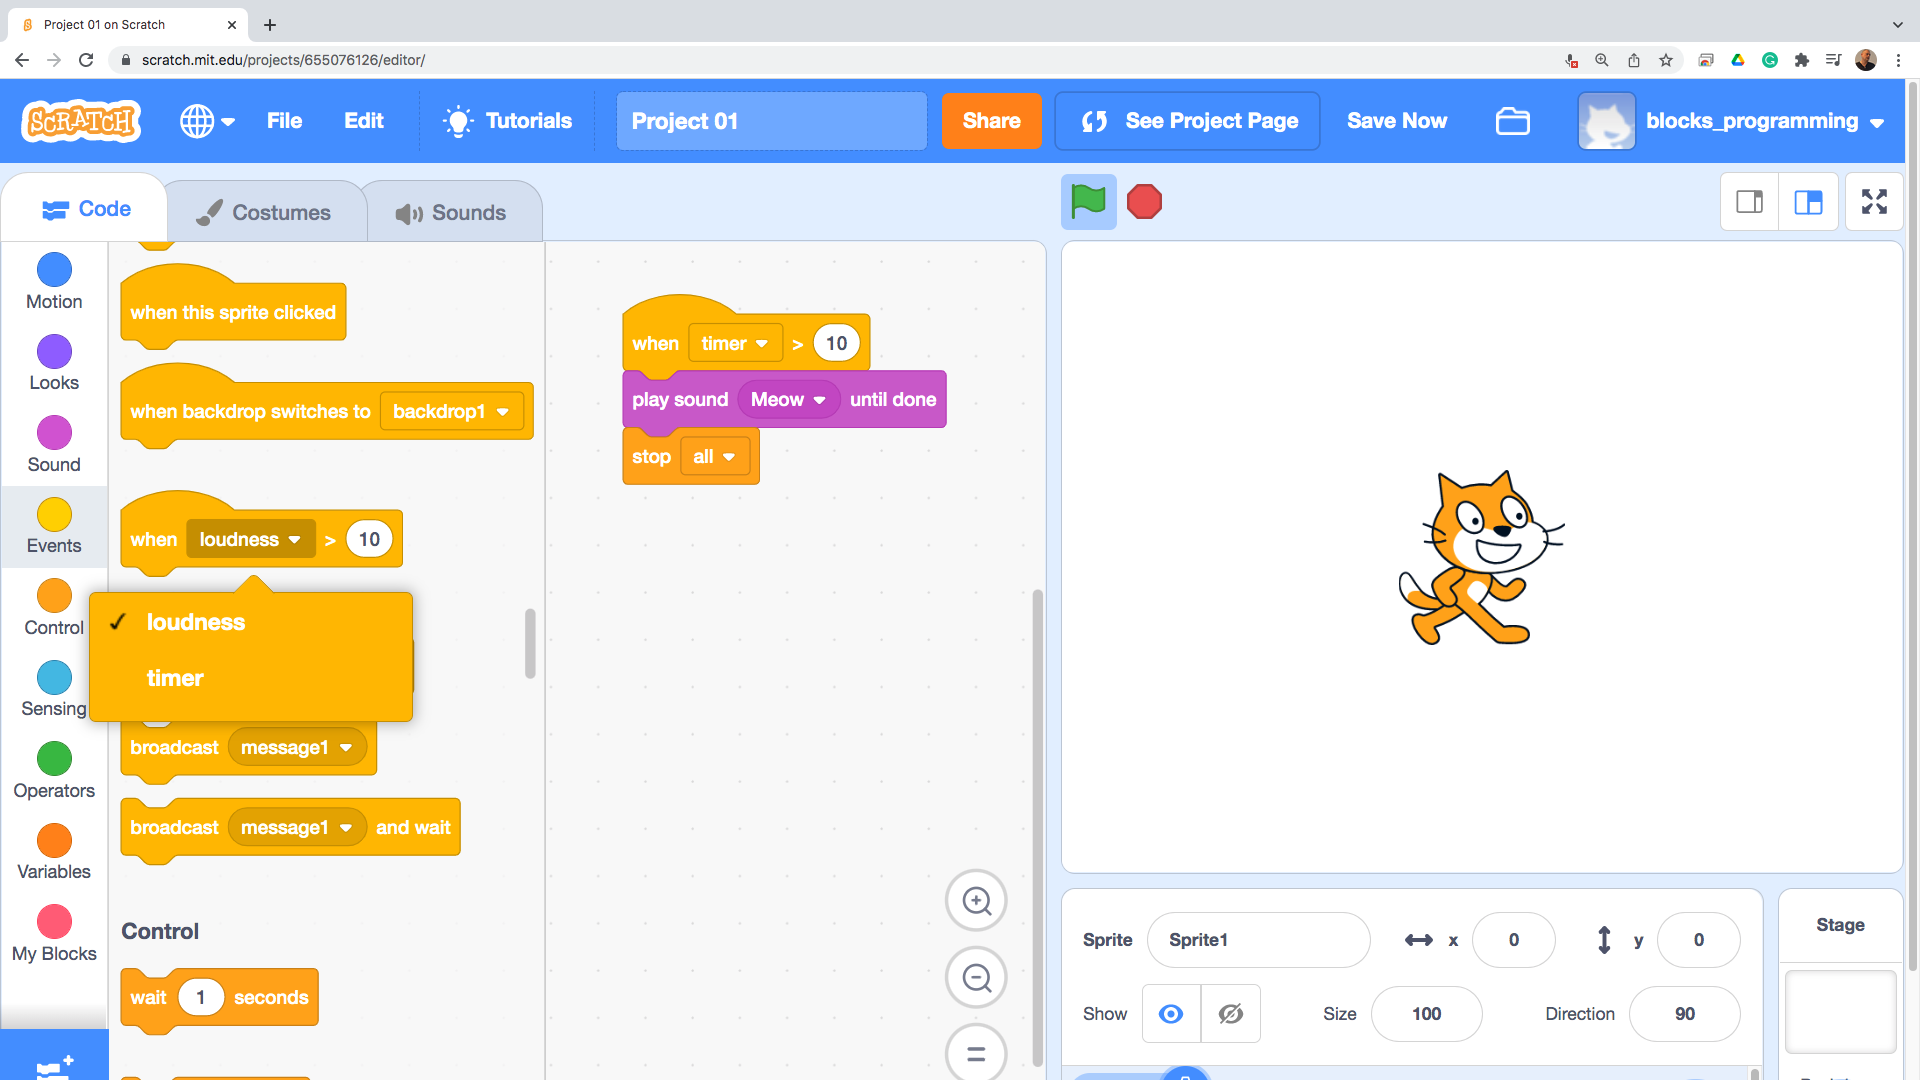
\includegraphics[width=1.0\linewidth,height=0.5\linewidth]{fig0082.png}
  \caption{Събитие от таймер или звук}
\label{fig0082}
\end{figure}

Работата със събития е свързана и с механизъм за предаване/получаване на съобщения. Един блок инструкции може да разпространи предварително дефинирано съобщение, а друг блок инструкции може да се абонира за получаването на точно този вид съобщение (Фиг. \ref{fig0083}).

\begin{figure}[H]
  \centering
  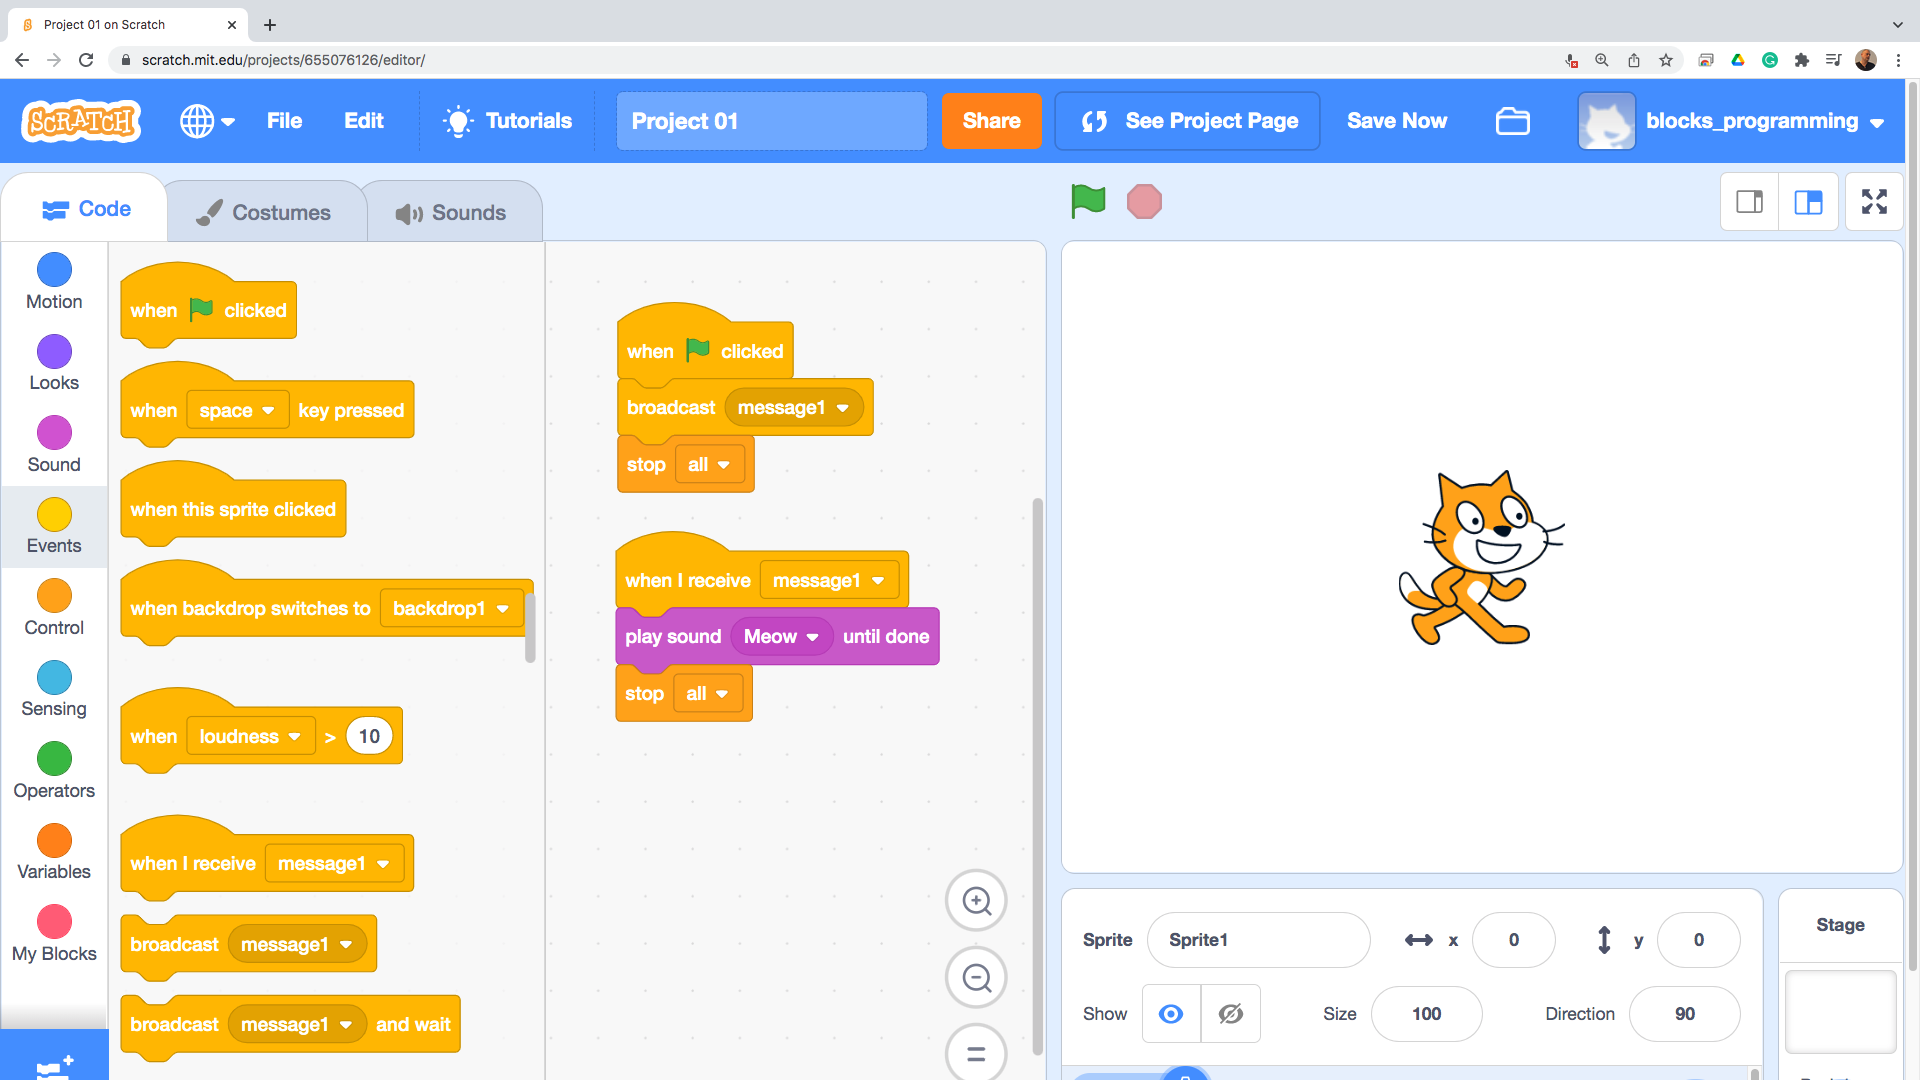
\includegraphics[width=1.0\linewidth,height=0.5\linewidth]{fig0083.png}
  \caption{Разпространяване и получаване на съобщения}
\label{fig0083}
\end{figure}

Тъй като работата с механизма за съобщения може да изисква синхронизация, то има отделно блокче, което разпространява съобщението и изчаква извършването на действията от прихващането му (Фиг. \ref{fig0084}). Програмистът може да създава различни съобщения, които да бъдат изпращани в различни ситуации. 

\begin{figure}[H]
  \centering
  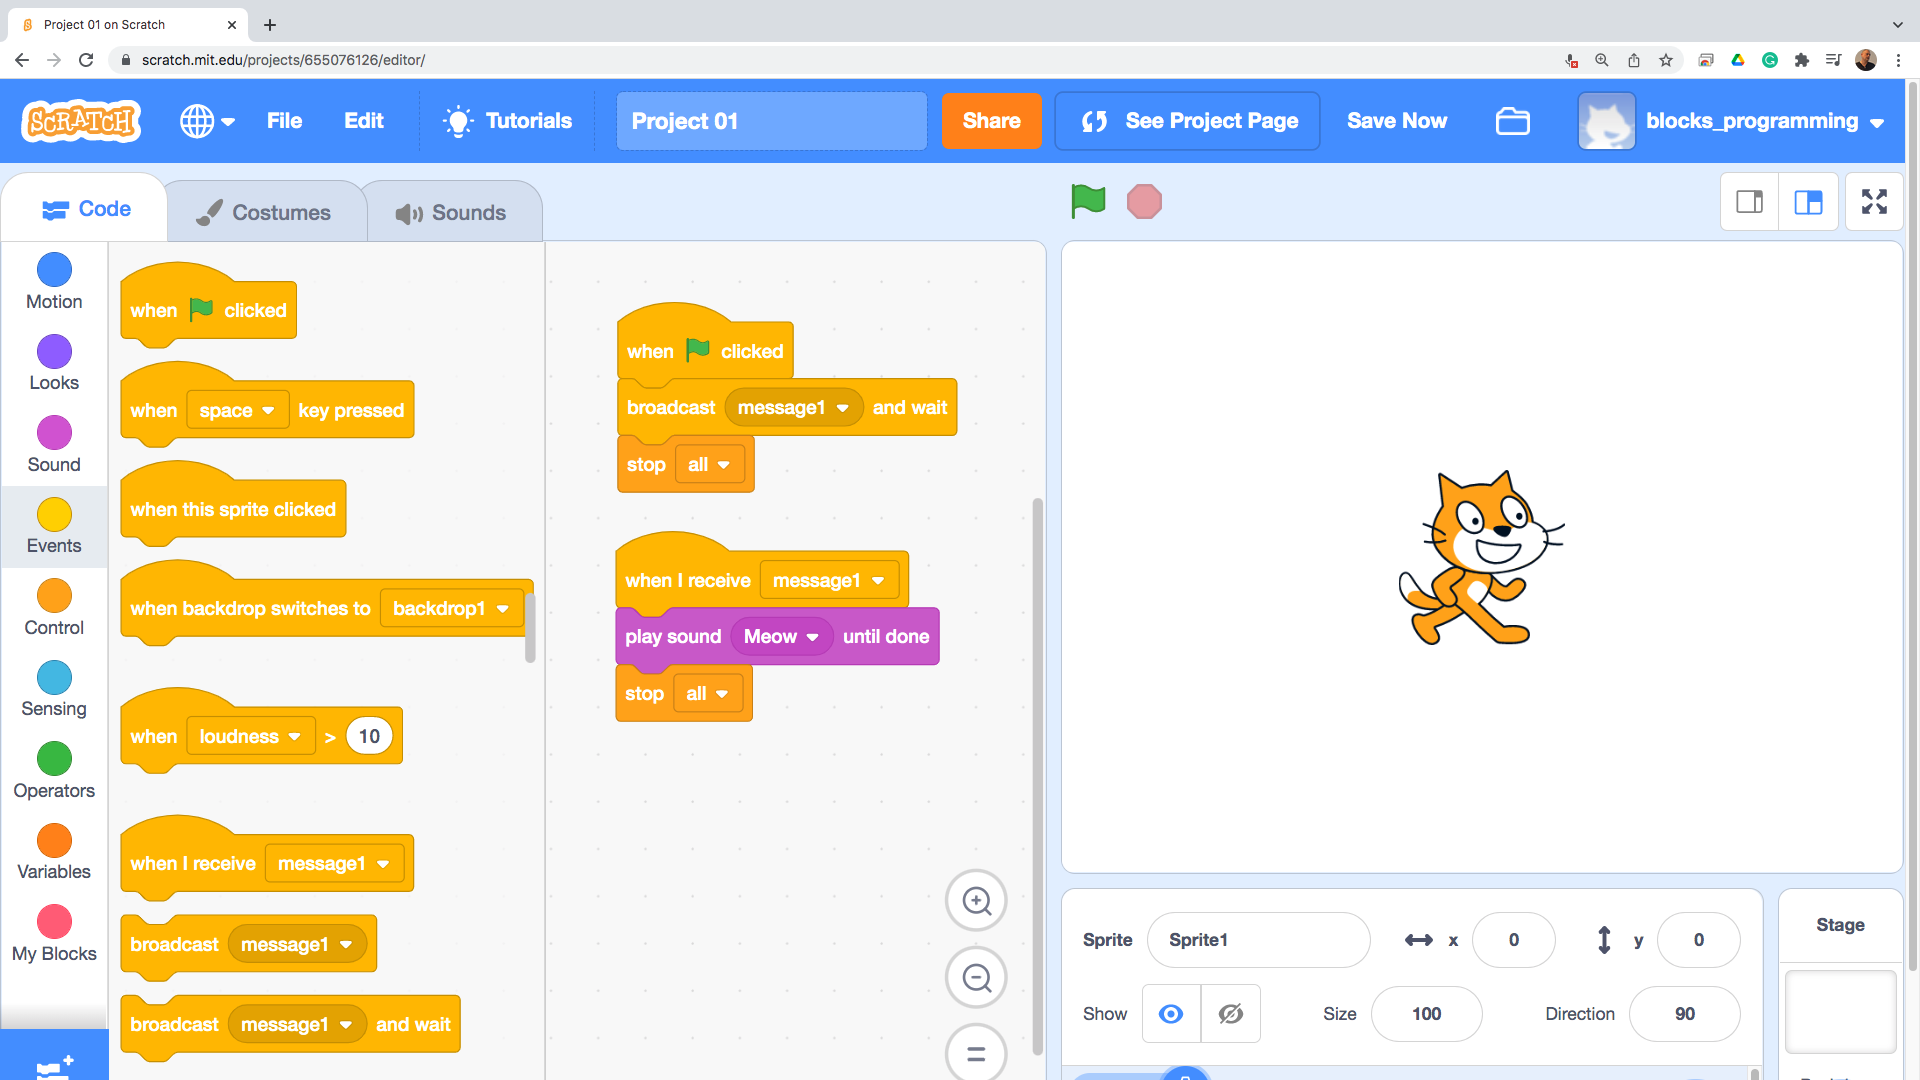
\includegraphics[width=1.0\linewidth,height=0.5\linewidth]{fig0084.png}
  \caption{Разпространяване на съобщение с изчакване}
\label{fig0084}
\end{figure}

Най-важните, а и най-полезните блокчета са организирани в групата на тъмно оранжевите. Това са блокчета, които определят по коя пътека на изпълнение ще се поеме, спрямо възможните избори за изпълнение на инструкции. Когато желанието е определено действие да се изпълни многократно, при зададен брой повторения, за тази цел има конкретно блокче (Фиг. \ref{fig0085}). В програмирането, многократните повторения се осъществяват с помощта на конструкции за цикъл, какъвто е случаят и с това блокче за повторения.

\begin{figure}[H]
  \centering
  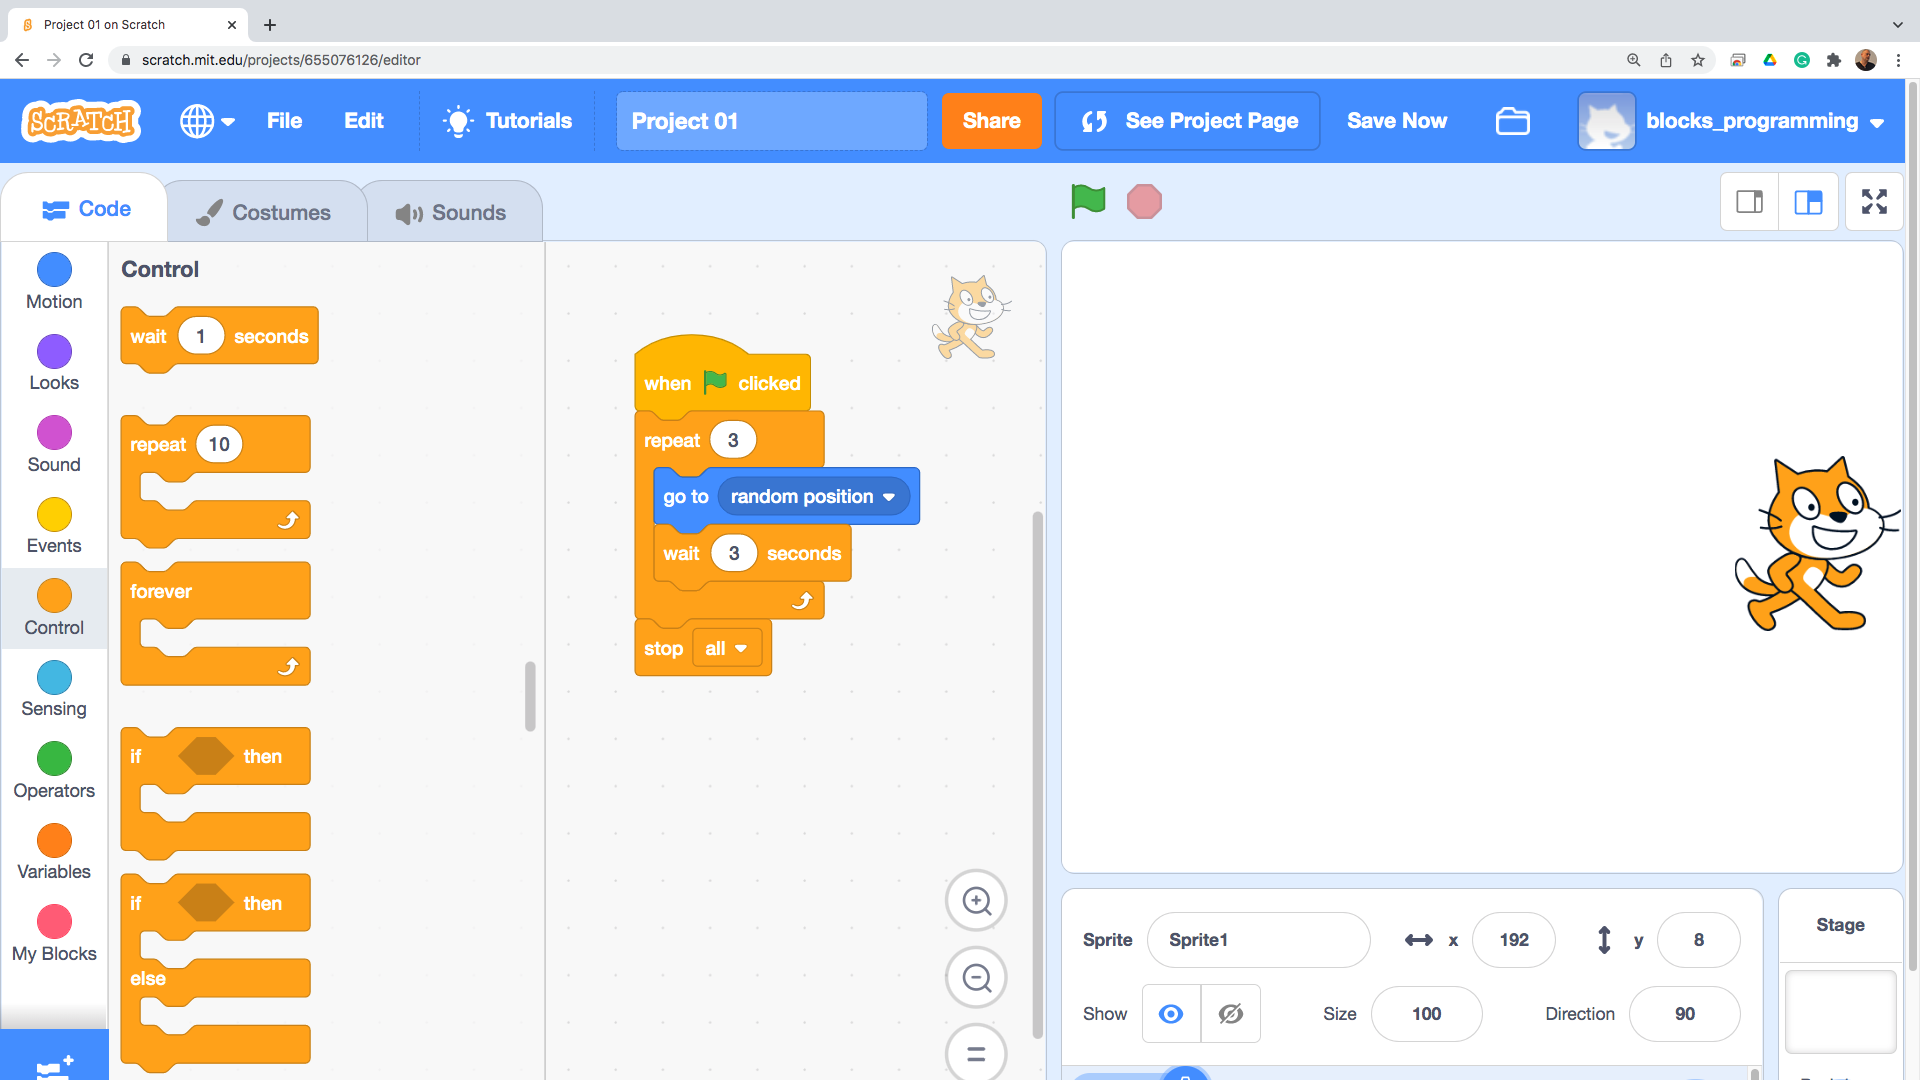
\includegraphics[width=1.0\linewidth,height=0.5\linewidth]{fig0085.png}
  \caption{Фиксиран брой повторения}
\label{fig0085}
\end{figure}

Думичката repeat от английски означава повтори. Числото в блокчето определя колко на брой повторения да бъдат изпълнени, а в слота на блочето се поставят инструкциите, които да бъдат повтаряни. В този пример, котето се премества на случайно избрани координати, след което следва изчакване от предварително определен брой секунди. В много редки ситуации има нужда от безкрайно повтарящ се цикъл, за което е предвидено отделно блокче (Фиг. \ref{fig0086}).

\begin{figure}[H]
  \centering
  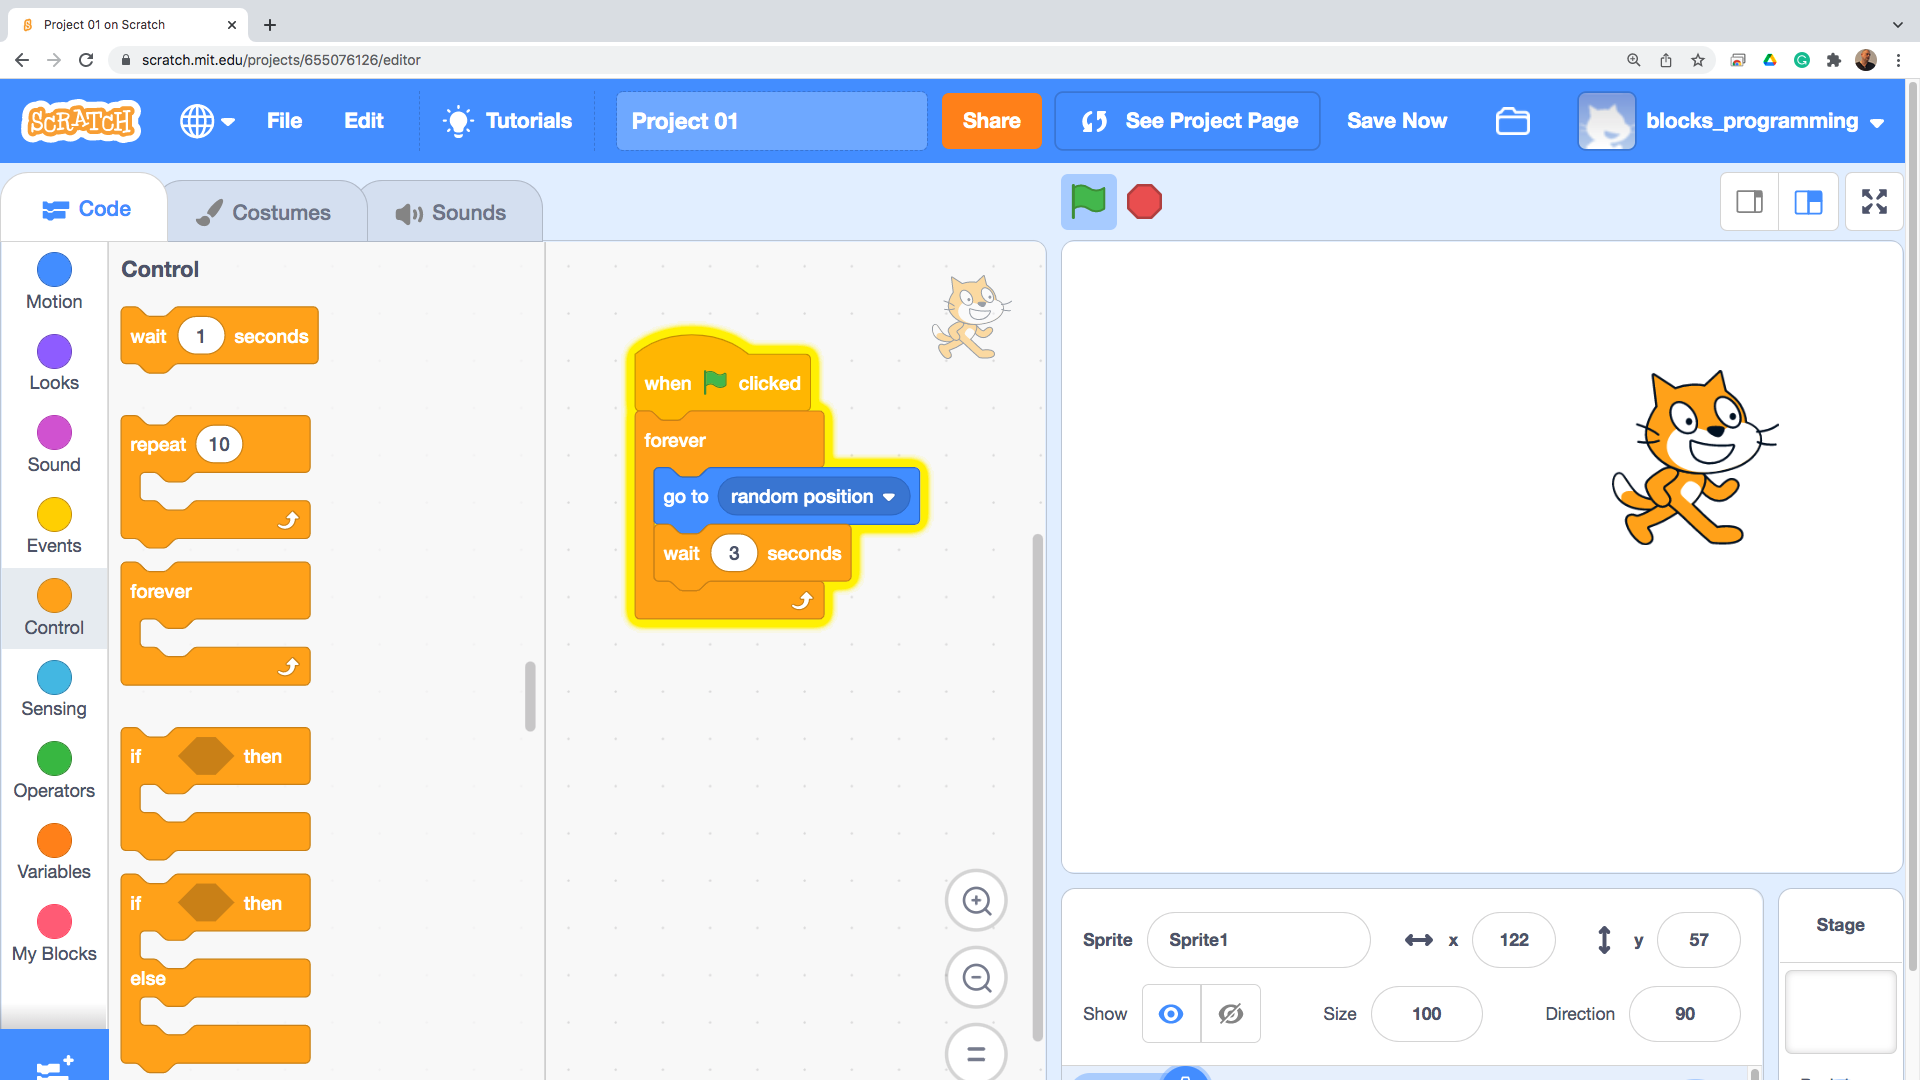
\includegraphics[width=1.0\linewidth,height=0.5\linewidth]{fig0086.png}
  \caption{Безкрайни повторения}
\label{fig0086}
\end{figure}

Следващото блокче е едно от най-важните блокчета в програмирането. То се нарича блокче за изпълнение при условие (Фиг. \ref{fig0087}) или условен преход. Съдържанието на блокчето се изпълнява само, ако условието в заглавната му част се изпълнява.

\begin{figure}[H]
  \centering
  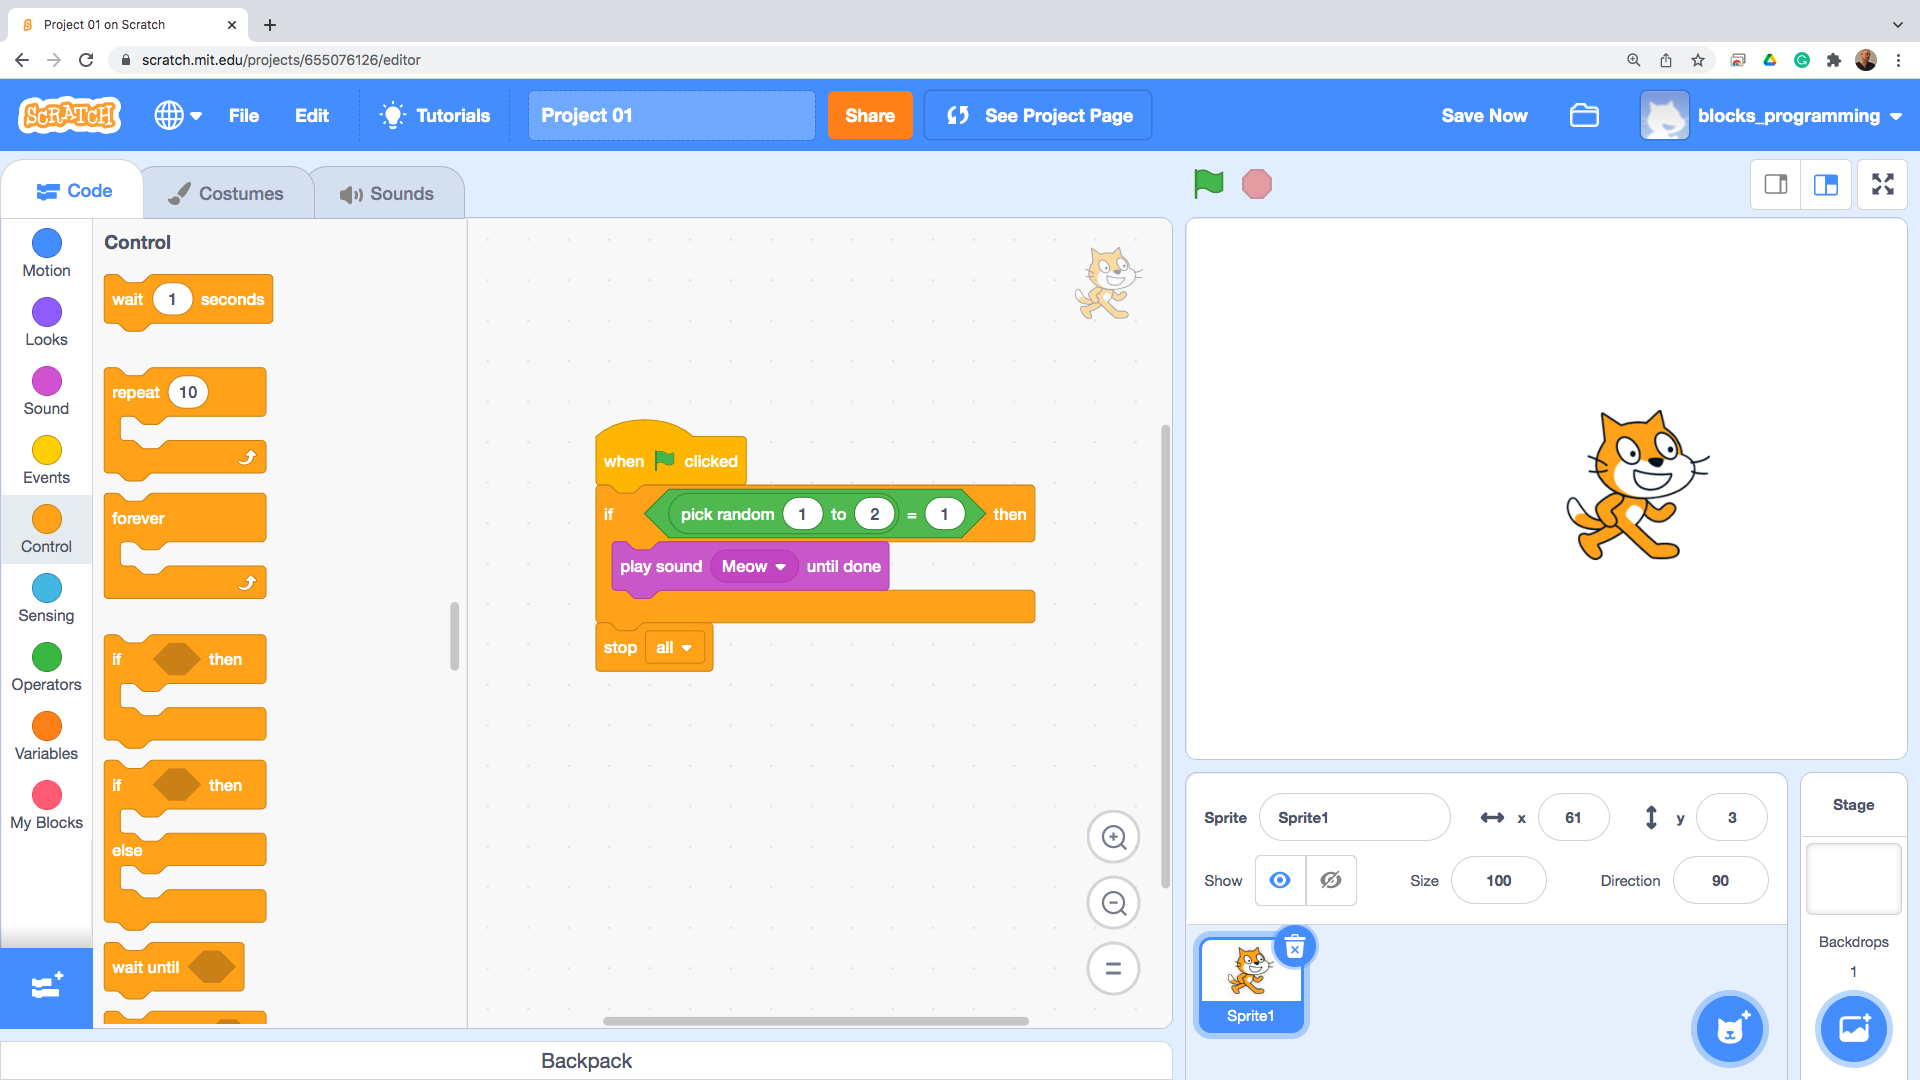
\includegraphics[width=1.0\linewidth,height=0.5\linewidth]{fig0087.png}
  \caption{Изпълнение при условие}
\label{fig0087}
\end{figure}

Това тъмно оранжево блокче не може да се използва само. То винаги е в съчетание с поне едно зелено блокче, а понякога и с две, както е в настоящия пример. Част от зелените блокчета са неправилни шестоъгълници и са направени така, че да пасват в заглавната част на някои от тъмно оранжевите блокчета. Самото шестоъгълно блокче има овален слот в който се поместват някои от зелените овални блокчета. В примера е избрано зелено блокче, което изисква равенство към конкретно число, а за овалното блокче се ползва генератор на случайни числа, според предварително зададен интервал. Ако условието в заглавната част на блокчето за условен преход не бъде изпълнено, то тялото се пропуска и се преминава към следващите инструкции, след блочкето. Блокчето за условен преход има и вариант в който се предвиждат слотове за изпълнение и на двете възможности – вярно условие или невярно условие (Фиг. \ref{fig0088}). Ако условието е изпълнено, се изпълнява първият блок с инструкции. Ако условието не е изпълнено, се изпълнява вторият блок с инструкции.

\begin{figure}[H]
  \centering
  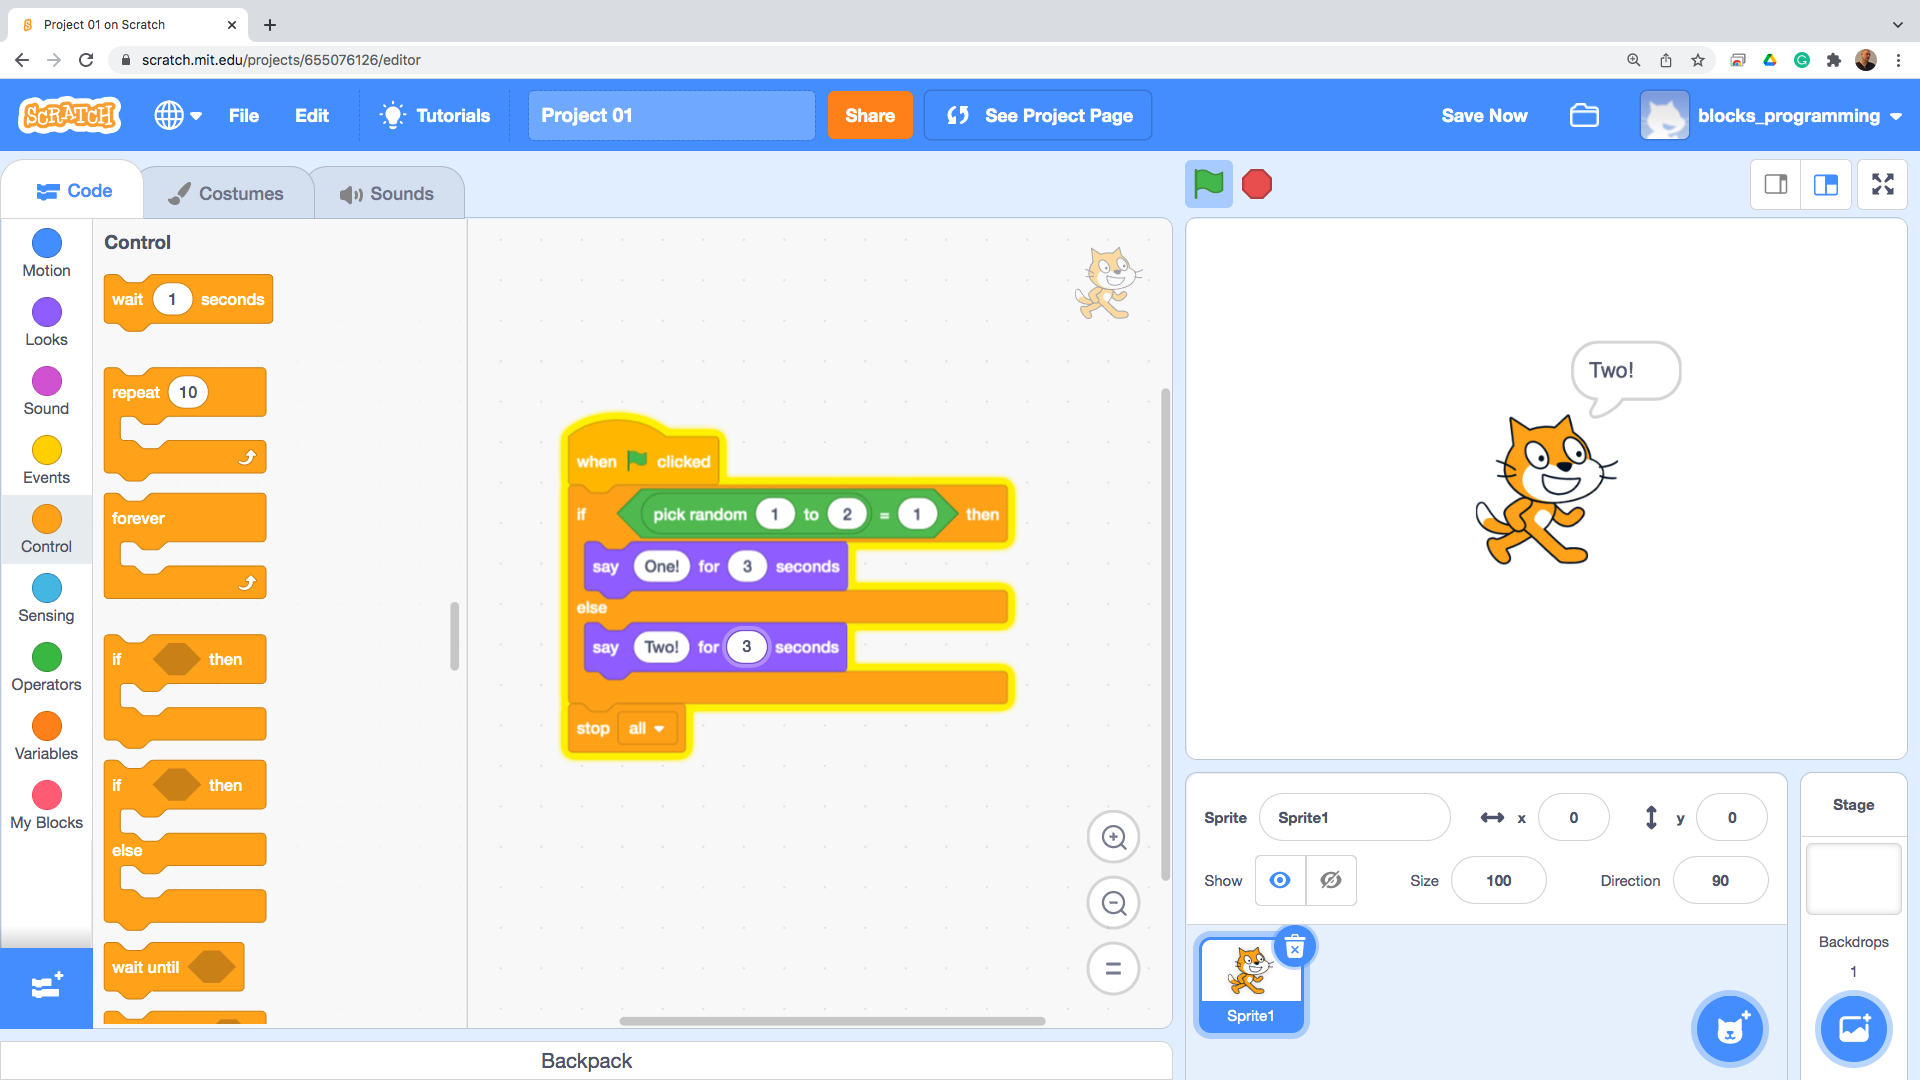
\includegraphics[width=1.0\linewidth,height=0.5\linewidth]{fig0088.png}
  \caption{Изпълнение при условие с алтернатива}
\label{fig0088}
\end{figure}

Следващото интересно блокче прави изчакване докато се случи определено събитие. В случая, събитието е спрайтът да бъде докоснат с мишката (Фиг. \ref{fig0089}). Случи ли се това докосване, изпълнението на програмата продължава към следващото блокче. Какво събитие се очаква е определено с допълнително блокче (светло синьо), което има формата на неправилен шестоъгълник.

\begin{figure}[H]
  \centering
  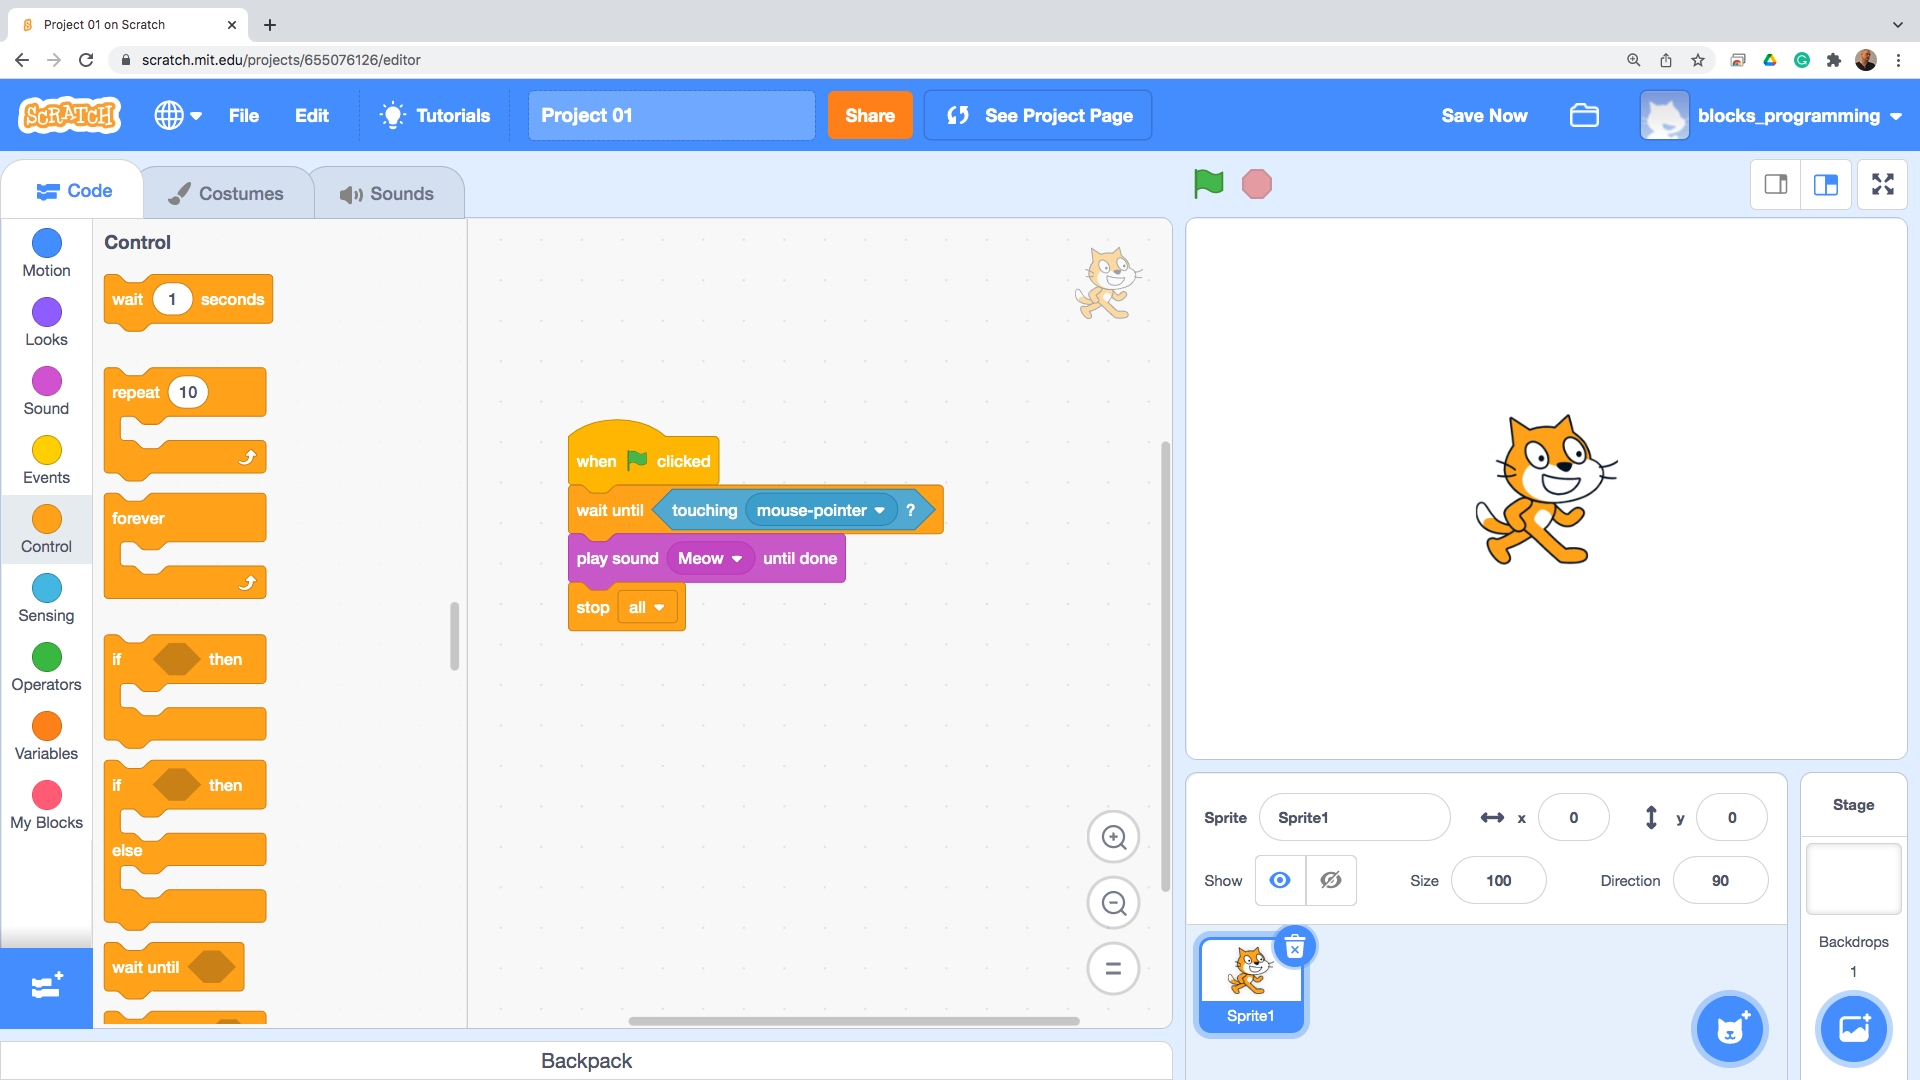
\includegraphics[width=1.0\linewidth,height=0.5\linewidth]{fig0089.png}
  \caption{Изчакване на условие}
\label{fig0089}
\end{figure}

Последните три блокчета в групата на тъмно оранжевите трябва да се демонстрират заедно (Фиг. \ref{fig0090}). Първото блокче задава нова верига от инструкции, когато определен спрай бъде клониран (копие на оригиналния спрайт). Второто блокче служи за клониране на текущия спрайт. А третото блокче служи за изтриване на текущия спрайт. 

\begin{figure}[H]
  \centering
  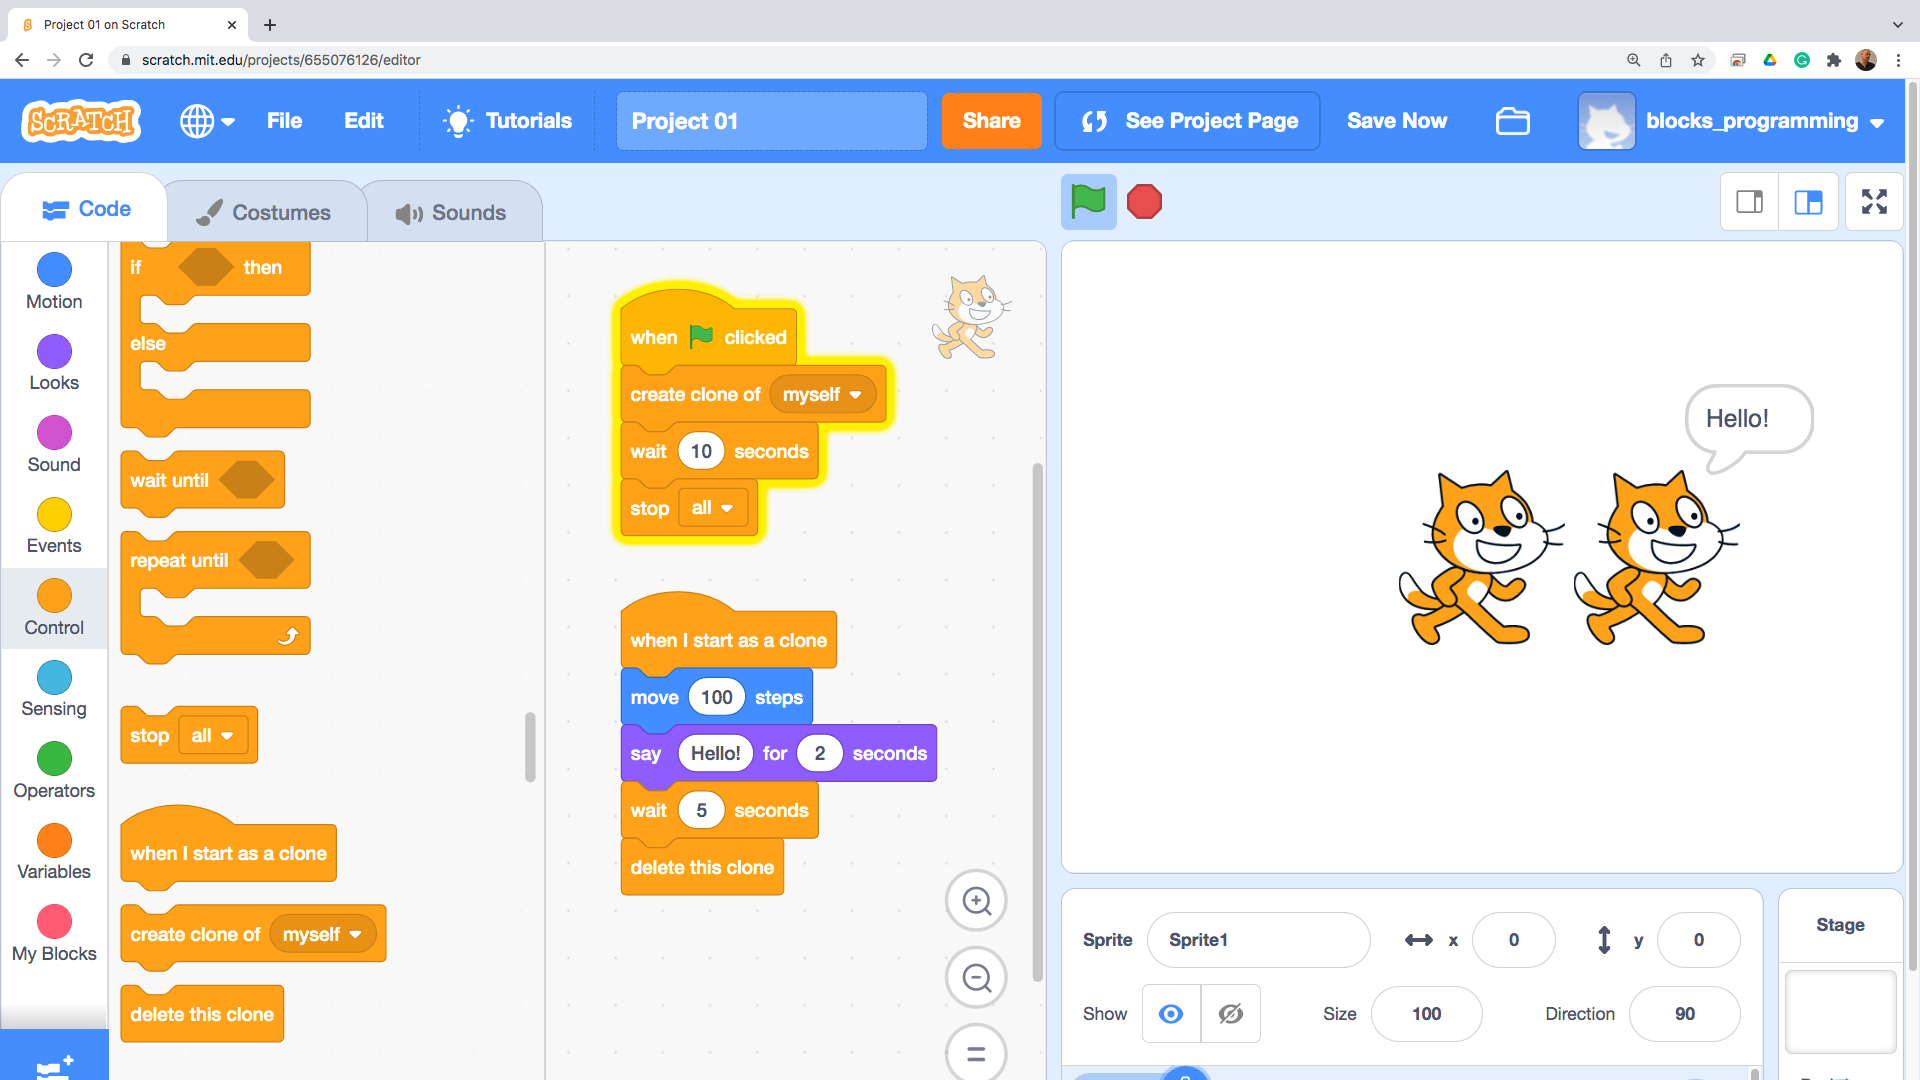
\includegraphics[width=1.0\linewidth,height=0.5\linewidth]{fig0090.png}
  \caption{Клониране на спрайтове}
\label{fig0090}
\end{figure}
\newpage
\addcontentsline{toc}{chapter}{Заключение}
\chapter*{Заключение}
\thispagestyle{empty}

Блоковото програмиране е ефективен и достъпен начин за запознаване на децата с концепциите за кодиране. Чрез разбиването на програмирането на визуални блокове, децата могат да се научат да сглобяват малки програми, без да се притесняват за синтаксис или грешки при въвеждане. Програмните среди Scratch и App Inventor са доказал се в практиката инструменти за преподаване на блоково програмиране на деца. Интуитивният интерфейс и цветните блокове на Scratch го правят идеален вариант за по-малки деца, докато способността на App Inventor да създава реални мобилни приложения може да се хареса на по-големите. Книгата предоставя изчерпателно ръководство за изучаване на блоково програмиране със Scratch и App Inventor. Обхваща проектиране и създаване на игри, създаване на мобилни приложения и други. Книгата също така включва инструкции стъпка по стъпка и много визуални примери, които да помогнат на децата да разберат концепциите за програмиране. Децата могат да развият основни умения като решаване на проблеми, логическо мислене и креативност чрез блоково програмиране. Тези умения могат да бъдат приложени в бъдещи начинания, включително компютърни науки и други области от науката, технологиите, инженерството и математиката. Като цяло, книгата за блоково програмиране за деца със Scratch и App Inventor е отличен ресурс за родители и преподаватели, които искат да запознаят децата с възможностите на програмирането. Използвайки визуални блокове и лесни за разбиране инструкции, децата могат да се научат да кодират по забавен и увлекателен начин, което ги подготвя за бъдещ успех в личен и професионален план.

\newpage

% Списък с използвана литература и източници на информация.
\addcontentsline{toc}{chapter}{Библиография}
\begin{thebibliography}{99}
\end{thebibliography}
\newpage

% Азбучен указател на използваните термини.
\printindex

% Задна корица.
\includepdf[pages=-]{covers/back}

\end{document}